\documentclass[11pt]{article}
\usepackage[margin=2cm]{geometry}
\usepackage{amsmath,amssymb}
\usepackage{graphicx}
\usepackage{booktabs}
\usepackage{array}
\usepackage{xcolor}
\usepackage[breakable]{tcolorbox}
\usepackage{enumitem}
\usepackage[hidelinks]{hyperref}
\allowdisplaybreaks
\setlength{\parindent}{0pt}
\setlength{\parskip}{4pt}
\definecolor{stepc}{HTML}{1F4E9E}
\definecolor{ansc}{HTML}{0B6E4F}
\newcommand{\solstep}[2]{\par\medskip{\color{stepc}\textbf{Step #1 --- #2}}\par\nopagebreak}
\newtcolorbox{probbox}[1]{colback=white,colframe=black!55,fonttitle=\bfseries,title={#1}}
\newtcolorbox{ansbox}{breakable,colback=ansc!6,colframe=ansc,fonttitle=\bfseries,title={Answer}}
\newtcolorbox{cardbox}[1]{breakable,colback=stepc!4,colframe=stepc,fonttitle=\bfseries,title={#1}}
\graphicspath{{../../../output/lecture1/1A_ac_transfer/}}
\title{Set 1A: AC Transfer Functions of RLC Networks}
\author{ECEN 325 --- Lecture 1 (Linear Network Analysis) practice set}
\date{}
\begin{document}
\maketitle

\textbf{What this set trains.} Finding $H(s)=V_o/V_i$ of a passive network with \emph{voltage dividers only},
turning it into Bode-ready form, sketching the magnitude Bode plot, and computing the steady-state sinusoidal
output. There are no DC sources here, so Step~2 of the pipeline is always trivial. Problems 1--6 are easy,
7--12 medium, 13--18 hard. Try each problem before looking at its solution.


\begin{cardbox}{The Lecture-1 pipeline (use it for every problem in this set)}
\textbf{Tools --- this is all the theory you need:}
\begin{enumerate}[label=\textbf{T\arabic*},leftmargin=2.2em,itemsep=1pt]
\item \emph{Impedances:} $Z_R=R$, $Z_C=\frac{1}{sC}$, $Z_L=sL$. Series: add. Parallel:
      $Z_a\parallel Z_b=\frac{Z_aZ_b}{Z_a+Z_b}$.
\item \emph{Voltage divider:} if $Z_{top}$ connects $V_{in}$ to a node and $Z_{bot}$ is everything from that
      node to ground, then $V_{node}=V_{in}\,\frac{Z_{bot}}{Z_{top}+Z_{bot}}$.
\item \emph{Divider between two voltages (DC):} a node tied to $V_a$ through $R_a$ and to $V_b$ through $R_b$ sits at
      $V=V_b+(V_a-V_b)\frac{R_b}{R_a+R_b}$, and looks like a source $V$ with resistance $R_a\parallel R_b$
      (its Thevenin pair).
\item \emph{Dependent sources:} a VCVS forces $V=kV_x$; a VCCS drives the current $gV_x$ through the impedance $Z$
      hanging on its node, so $V=\pm gV_x Z$ (sign from the arrow).
\item \emph{Sinusoids:} $A\sin(\omega t+\theta)\ \to\ |H(j\omega)|\,A\sin\big(\omega t+\theta+\angle H(j\omega)\big)$.
\item \emph{Bode rules:} a pole at $p$ bends the magnitude by $-20$\,dB/dec above $p$, a zero by $+20$\,dB/dec;
      $\frac{1}{1+s/p}$ is $0$\,dB below $p$; $\frac{s}{s+p}$ is $0$\,dB above $p$.
\end{enumerate}
\textbf{Steps:}
\begin{enumerate}[leftmargin=2.2em,itemsep=1pt]
\item \emph{Sources.} DC and AC both present $\Rightarrow$ superposition $V_o=V_{o,dc}+v_{o,ac}$.
\item \emph{DC circuit:} $V_i\to0$, $C\to$ open, $L\to$ short; reduce toward $V_o$ with T3.
\item \emph{AC circuit:} DC supplies $\to 0$ (rails become ground); merge parallel resistors.
\item \emph{Divider chain:} name the nodes from $V_i$ to $V_o$; $H=\prod$ (node-to-node ratios), each by T2 or T4,
      using the impedance seen looking right from each node.
\item \emph{Standard form:} simplify, find the roots, write $H=K\cdot\prod(\text{factors})$.
\item \emph{Bode:} start from the low-frequency slope, bend by $\pm20$\,dB/dec at each corner.
\item \emph{Output:} evaluate each factor at $s=j\omega_{in}$, multiply magnitudes, add angles, apply T5 and add $V_{o,dc}$.
\end{enumerate}
\end{cardbox}

\section*{Problems}
\subsection*{Easy problems}
\begin{probbox}{Problem 1A.1 \hfill Easy}
For the circuit below: (a) find the AC transfer function $H(s)=\dfrac{V_o(s)}{V_i(s)}$ and sketch its magnitude Bode plot; (b) find the steady-state output $V_o(t)$ for $V_i(t) = 2\sin\left(2\pi\cdot 1000\,t\right)$.
\begin{center}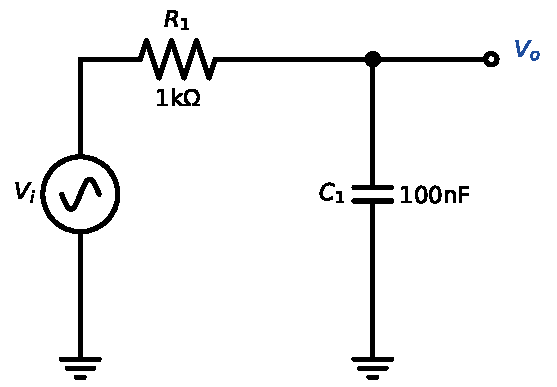
\includegraphics[width=0.8\linewidth,height=5.5cm,keepaspectratio]{p01_circuit}\end{center}
\end{probbox}

\begin{probbox}{Problem 1A.2 \hfill Easy}
For the circuit below: (a) find the AC transfer function $H(s)=\dfrac{V_o(s)}{V_i(s)}$ and sketch its magnitude Bode plot; (b) find the steady-state output $V_o(t)$ for $V_i(t) = 1\sin\left(2\pi\cdot 200\,t\right)$.
\begin{center}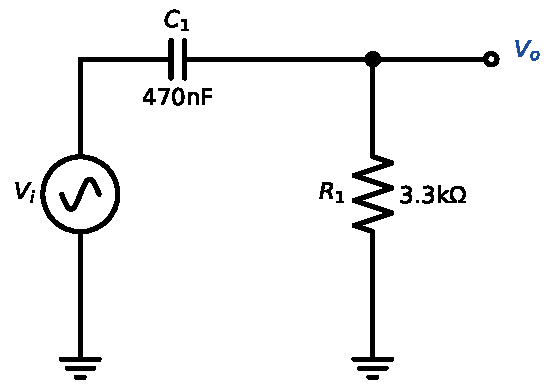
\includegraphics[width=0.8\linewidth,height=5.5cm,keepaspectratio]{p02_circuit}\end{center}
\end{probbox}

\begin{probbox}{Problem 1A.3 \hfill Easy}
For the circuit below: (a) find the AC transfer function $H(s)=\dfrac{V_o(s)}{V_i(s)}$ and sketch its magnitude Bode plot; (b) find the steady-state output $V_o(t)$ for $V_i(t) = 0.5\sin\left(2\pi\cdot 10000\,t\right)$.
\begin{center}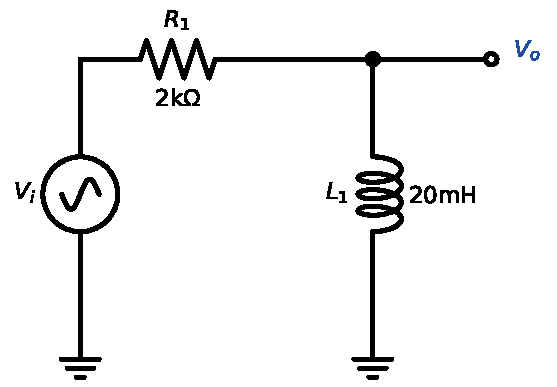
\includegraphics[width=0.8\linewidth,height=5.5cm,keepaspectratio]{p03_circuit}\end{center}
\end{probbox}

\begin{probbox}{Problem 1A.4 \hfill Easy}
For the circuit below: (a) find the AC transfer function $H(s)=\dfrac{V_o(s)}{V_i(s)}$ and sketch its magnitude Bode plot; (b) find the steady-state output $V_o(t)$ for $V_i(t) = 3\cos\left(2\pi\cdot 5000\,t\right)$.
\begin{center}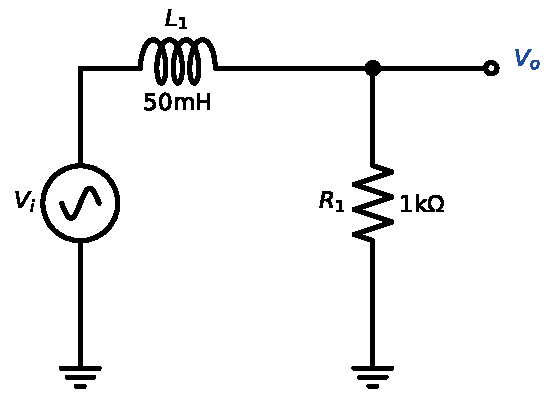
\includegraphics[width=0.8\linewidth,height=5.5cm,keepaspectratio]{p04_circuit}\end{center}
\end{probbox}

\begin{probbox}{Problem 1A.5 \hfill Easy}
For the circuit below: (a) find the AC transfer function $H(s)=\dfrac{V_o(s)}{V_i(s)}$ and sketch its magnitude Bode plot; (b) find the steady-state output $V_o(t)$ for $V_i(t) = 1\sin\left(2\pi\cdot 2000\,t\right)$.
\begin{center}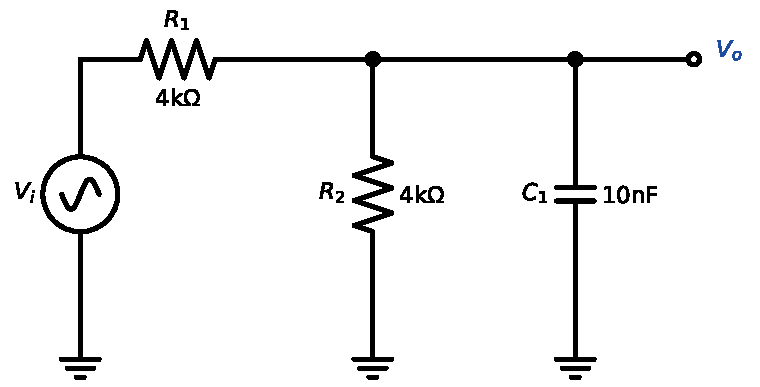
\includegraphics[width=0.8\linewidth,height=5.5cm,keepaspectratio]{p05_circuit}\end{center}
\end{probbox}

\begin{probbox}{Problem 1A.6 \hfill Easy}
For the circuit below: (a) find the AC transfer function $H(s)=\dfrac{V_o(s)}{V_i(s)}$ and sketch its magnitude Bode plot; (b) find the steady-state output $V_o(t)$ for $V_i(t) = 0.2\sin\left(2\pi\cdot 50\,t\right)$.
\begin{center}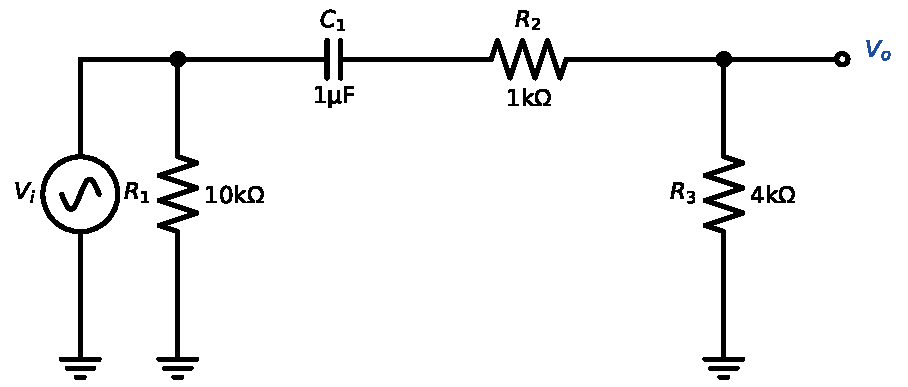
\includegraphics[width=0.8\linewidth,height=5.5cm,keepaspectratio]{p06_circuit}\end{center}
\end{probbox}

\subsection*{Medium problems}
\begin{probbox}{Problem 1A.7 \hfill Medium}
For the circuit below: (a) find the AC transfer function $H(s)=\dfrac{V_o(s)}{V_i(s)}$ and sketch its magnitude Bode plot; (b) find the steady-state output $V_o(t)$ for $V_i(t) = 1\sin\left(2\pi\cdot 500\,t\right)$.
\begin{center}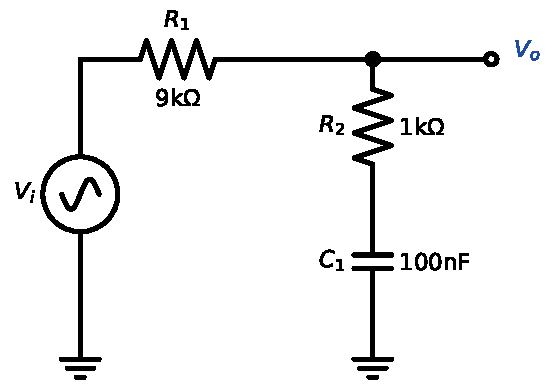
\includegraphics[width=0.8\linewidth,height=5.5cm,keepaspectratio]{p07_circuit}\end{center}
\end{probbox}

\begin{probbox}{Problem 1A.8 \hfill Medium}
For the circuit below: (a) find the AC transfer function $H(s)=\dfrac{V_o(s)}{V_i(s)}$ and sketch its magnitude Bode plot; (b) find the steady-state output $V_o(t)$ for $V_i(t) = 0.5\sin\left(2\pi\cdot 5000\,t\right)$.
\begin{center}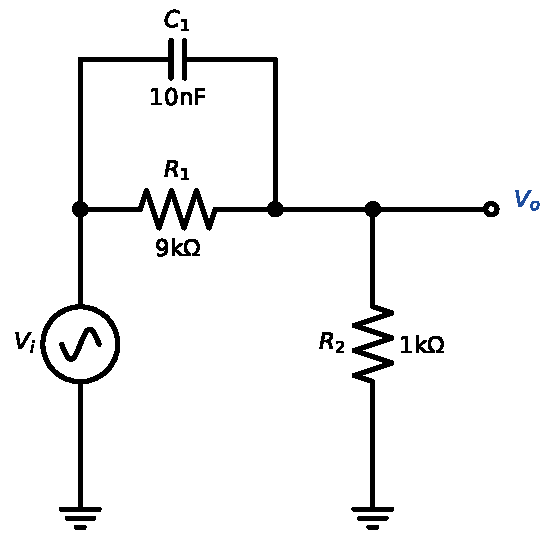
\includegraphics[width=0.8\linewidth,height=5.5cm,keepaspectratio]{p08_circuit}\end{center}
\end{probbox}

\begin{probbox}{Problem 1A.9 \hfill Medium}
For the circuit below: (a) find the AC transfer function $H(s)=\dfrac{V_o(s)}{V_i(s)}$ and sketch its magnitude Bode plot; (b) find the steady-state output $V_o(t)$ for $V_i(t) = 1\sin\left(2\pi\cdot 1000\,t\right)$.
\begin{center}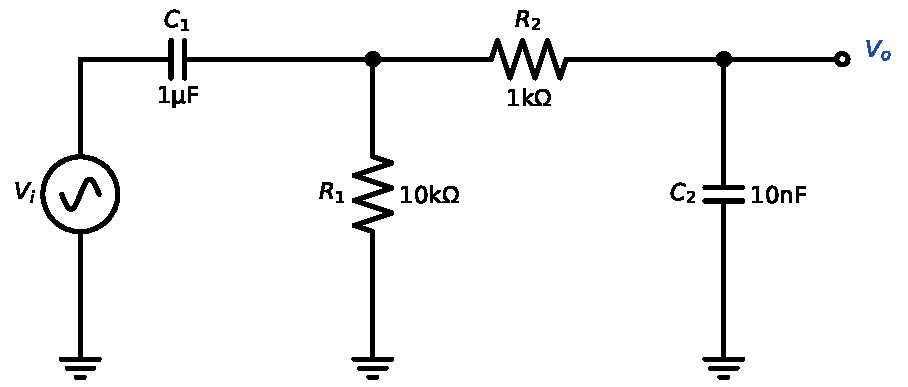
\includegraphics[width=0.8\linewidth,height=5.5cm,keepaspectratio]{p09_circuit}\end{center}
\end{probbox}

\begin{probbox}{Problem 1A.10 \hfill Medium}
For the circuit below: (a) find the AC transfer function $H(s)=\dfrac{V_o(s)}{V_i(s)}$ and sketch its magnitude Bode plot; (b) find the steady-state output $V_o(t)$ for $V_i(t) = 1\sin\left(2\pi\cdot 3000\,t\right)$.
\begin{center}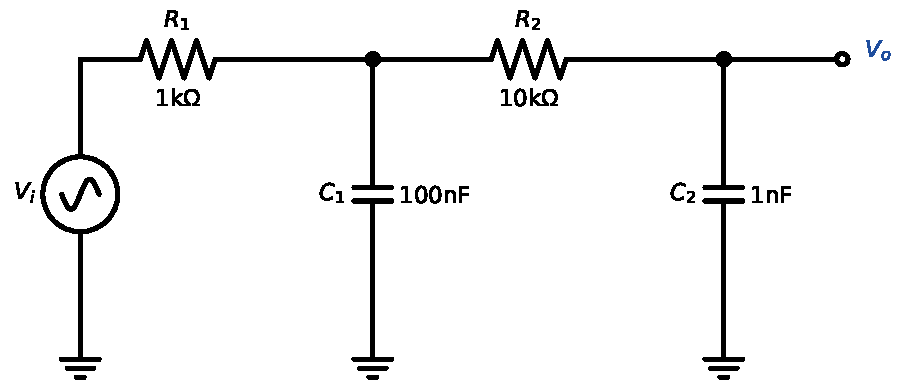
\includegraphics[width=0.8\linewidth,height=5.5cm,keepaspectratio]{p10_circuit}\end{center}
\end{probbox}

\begin{probbox}{Problem 1A.11 \hfill Medium}
For the circuit below: (a) find the AC transfer function $H(s)=\dfrac{V_o(s)}{V_i(s)}$ and sketch its magnitude Bode plot; (b) find the steady-state output $V_o(t)$ for $V_i(t) = 2\sin\left(2\pi\cdot 1000\,t\right)$.
\begin{center}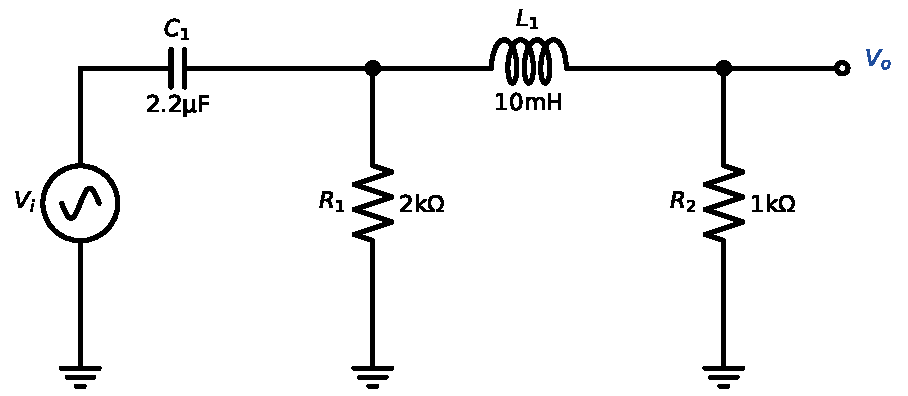
\includegraphics[width=0.8\linewidth,height=5.5cm,keepaspectratio]{p11_circuit}\end{center}
\end{probbox}

\begin{probbox}{Problem 1A.12 \hfill Medium}
For the circuit below: (a) find the AC transfer function $H(s)=\dfrac{V_o(s)}{V_i(s)}$ and sketch its magnitude Bode plot; (b) find the steady-state output $V_o(t)$ for $V_i(t) = 1\sin\left(2\pi\cdot 1000\,t\right)$.
\begin{center}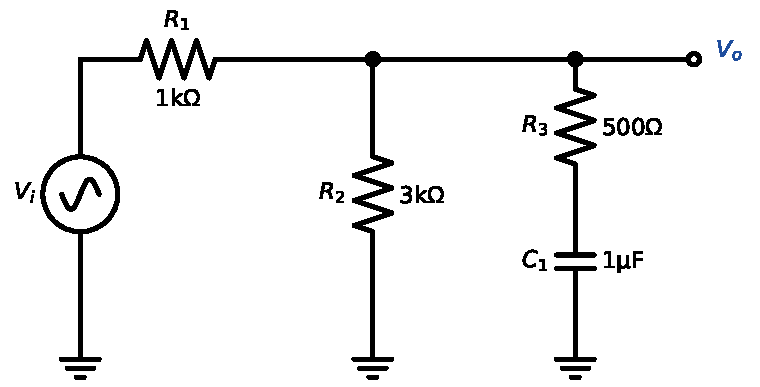
\includegraphics[width=0.8\linewidth,height=5.5cm,keepaspectratio]{p12_circuit}\end{center}
\end{probbox}

\subsection*{Hard problems}
\begin{probbox}{Problem 1A.13 \hfill Hard}
For the circuit below: (a) find the AC transfer function $H(s)=\dfrac{V_o(s)}{V_i(s)}$ and sketch its magnitude Bode plot; (b) find the steady-state output $V_o(t)$ for $V_i(t) = 1\cos\left(2\pi\cdot 2000\,t+\frac{\pi}{4}\right)$.
\begin{center}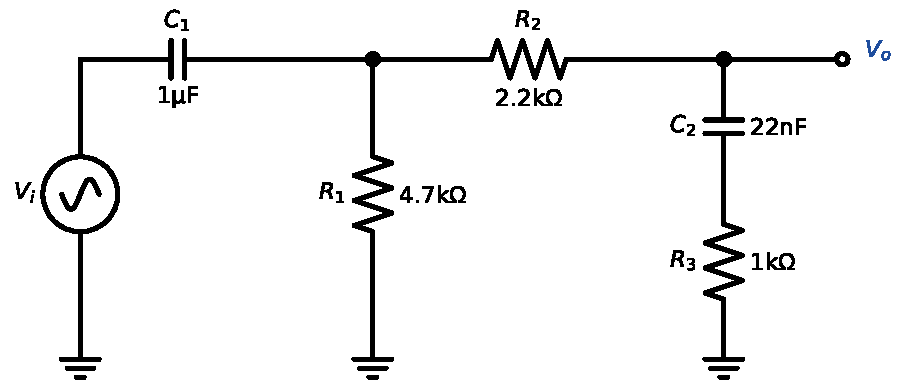
\includegraphics[width=0.8\linewidth,height=5.5cm,keepaspectratio]{p13_circuit}\end{center}
\end{probbox}

\begin{probbox}{Problem 1A.14 \hfill Hard}
For the circuit below: (a) find the AC transfer function $H(s)=\dfrac{V_o(s)}{V_i(s)}$ and sketch its magnitude Bode plot; (b) find the steady-state output $V_o(t)$ for $V_i(t) = 1\sin\left(2\pi\cdot 1000\,t+\frac{\pi}{3}\right)$.
\begin{center}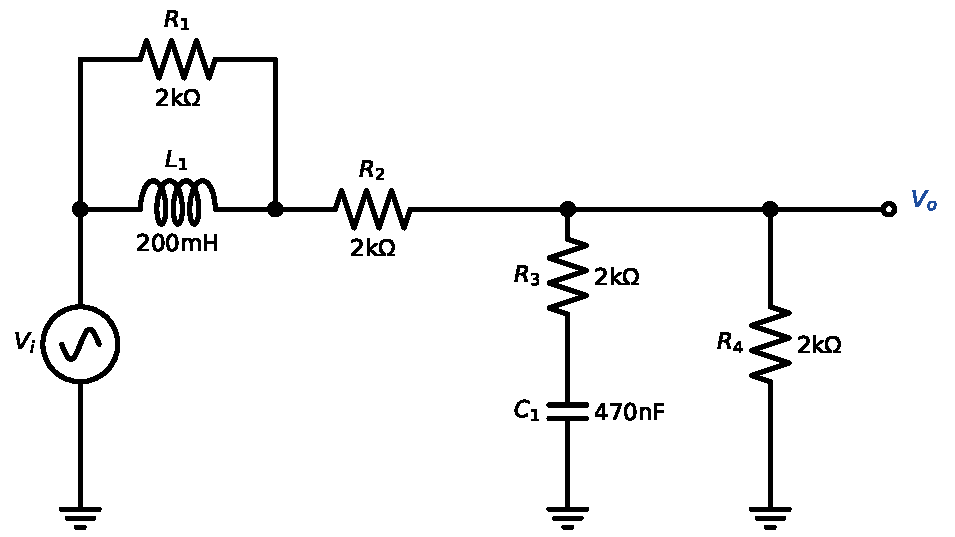
\includegraphics[width=0.8\linewidth,height=5.5cm,keepaspectratio]{p14_circuit}\end{center}
\end{probbox}

\begin{probbox}{Problem 1A.15 \hfill Hard}
For the circuit below: (a) find the AC transfer function $H(s)=\dfrac{V_o(s)}{V_i(s)}$ and sketch its magnitude Bode plot; (b) find the steady-state output $V_o(t)$ for $V_i(t) = 0.5\sin\left(2\pi\cdot 2000\,t\right)$.
\begin{center}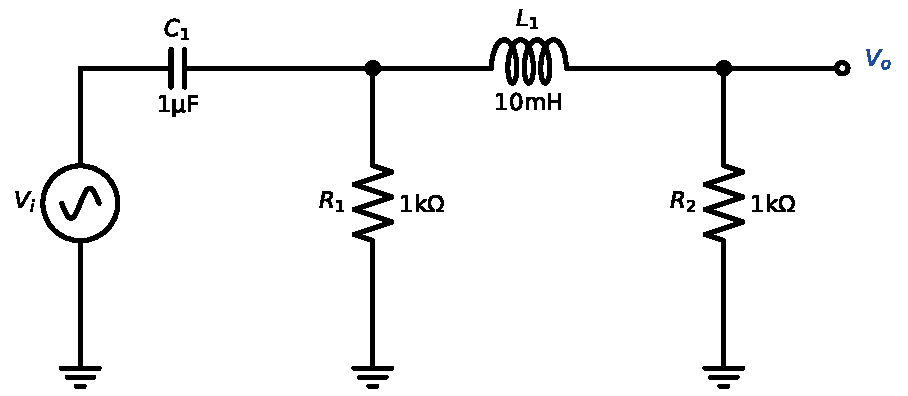
\includegraphics[width=0.8\linewidth,height=5.5cm,keepaspectratio]{p15_circuit}\end{center}
\end{probbox}

\begin{probbox}{Problem 1A.16 \hfill Hard}
For the circuit below: (a) find the AC transfer function $H(s)=\dfrac{V_o(s)}{V_i(s)}$ and sketch its magnitude Bode plot; (b) find the steady-state output $V_o(t)$ for $V_i(t) = 1\sin\left(2\pi\cdot 1000\,t\right)$.
\begin{center}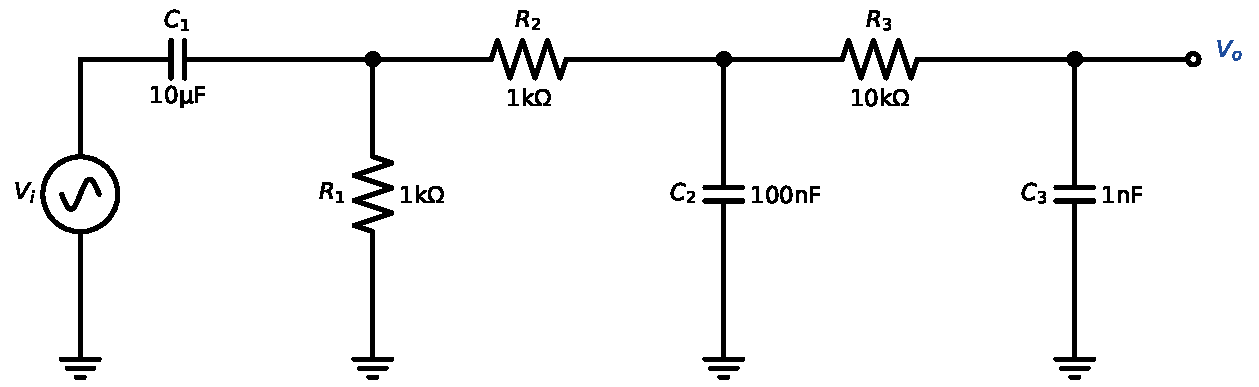
\includegraphics[width=0.8\linewidth,height=5.5cm,keepaspectratio]{p16_circuit}\end{center}
\end{probbox}

\begin{probbox}{Problem 1A.17 \hfill Hard}
For the circuit below: (a) find the AC transfer function $H(s)=\dfrac{V_o(s)}{V_i(s)}$ and sketch its magnitude Bode plot; (b) find the steady-state output $V_o(t)$ for $V_i(t) = 1\sin\left(2\pi\cdot 500\,t\right)$. Note that $V_o$ is \emph{not} at the right end: the branch to its right loads it.
\begin{center}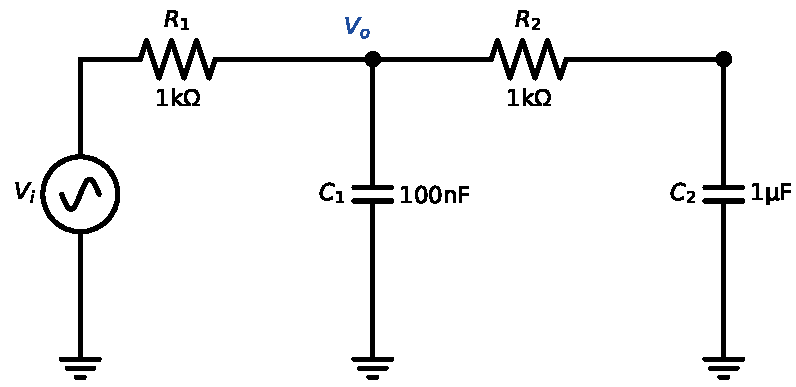
\includegraphics[width=0.8\linewidth,height=5.5cm,keepaspectratio]{p17_circuit}\end{center}
\end{probbox}

\begin{probbox}{Problem 1A.18 \hfill Hard}
For the circuit below: (a) find the AC transfer function $H(s)=\dfrac{V_o(s)}{V_i(s)}$ and sketch its magnitude Bode plot; (b) find the steady-state output $V_o(t)$ for $V_i(t) = 1\sin\left(2\pi\cdot 2000\,t-\frac{\pi}{6}\right)$.
\begin{center}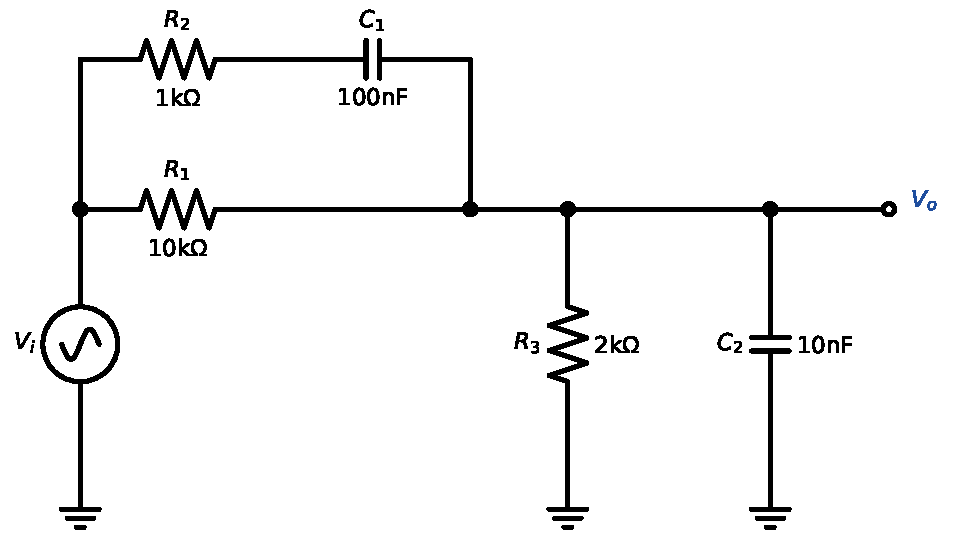
\includegraphics[width=0.8\linewidth,height=5.5cm,keepaspectratio]{p18_circuit}\end{center}
\end{probbox}

\newpage
\section*{Solutions}
Every solution follows the same seven steps of the pipeline card.
\newpage
\subsection*{Solution 1A.1 \hfill Easy}
\begin{center}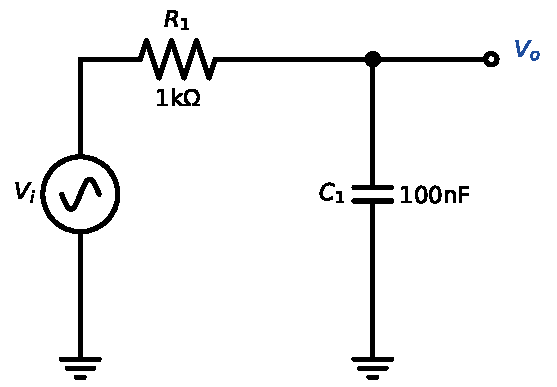
\includegraphics[width=0.8\linewidth,height=4.5cm,keepaspectratio]{p01_circuit}\end{center}
\solstep{1}{Identify the sources}Independent sources: the AC input $V_i(t)$. There is no DC source, so $V_{o,dc}=0$ and $V_o(t)=v_{o,ac}(t)$: Step 2 is skipped.
\solstep{2}{DC circuit}No DC sources: $V_{o,dc}=0$.
\solstep{3}{AC circuit}Replace every capacitor by $\frac{1}{sC}$ and every inductor by $sL$.
AC equivalent circuit (nodes named for the next step):
\begin{center}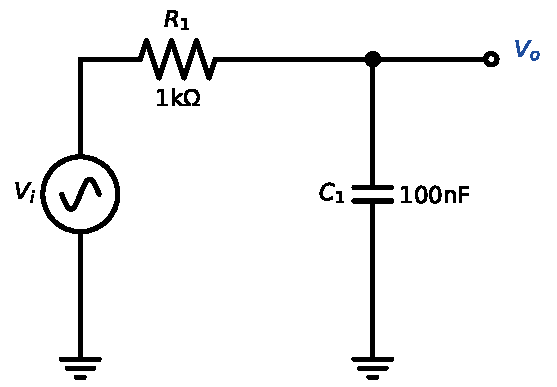
\includegraphics[width=0.95\linewidth,height=5.2cm,keepaspectratio]{p01_ac}\end{center}

\solstep{4}{Transfer function by a chain of dividers}Walk from the input to the output through the named nodes: $V_{i} \to V_{o}$. There is a single link, so $H(s)$ is just one voltage divider (tool T2).
Now each link. {\small (Algebra tip: to simplify a fraction that contains fractions, multiply its top and bottom by every inner denominator; then divide top and bottom by the leading coefficient of the denominator so that it starts with a plain $s^n$.)}
\begin{align*}
\frac{V_{o}}{V_{i}} &= \frac{\frac{1}{sC_{1}}}{R_{1} + \frac{1}{sC_{1}}} = \dfrac{10000}{s + 10000}
\end{align*}

So:\[
H(s) = \dfrac{10000}{s + 10000}
\]

\solstep{5}{Standard (Bode-ready) form}Find the roots. Every root $s=-p$ of the denominator is a \emph{pole}, every root $s=-z$ of the numerator is a \emph{zero}; $|p|$ and $|z|$ are the corner frequencies (rad/s).
\begin{itemize}[leftmargin=*,itemsep=2pt]
\item Denominator: $s + 10000$; $s + 10000 = 0 \Rightarrow s = -10000$.
\end{itemize}

Factored form (leading coefficient in front):
\[
H(s) = 10000\,\dfrac{1}{(s+10000)}
\]

Bode-ready form: rewrite every $(s+p) = p\left(1+\frac{s}{p}\right)$ and $(s+z) = z\left(1+\frac{s}{z}\right)$, and collect all constants into $K$. Then every factor except $K$ is $\approx 1$ inside the pass-band:
\[
H(s) = 1\,\dfrac{1}{1+\dfrac{s}{2\pi\cdot 1.59\mathrm{k}}},\qquad K = 1
\]

\begin{center}\renewcommand{\arraystretch}{1.35}
\begin{tabular}{cccc}
\toprule
type & $\omega_c$ (rad/s) & $f_c=\omega_c/2\pi$ & slope change \\
\midrule
pole & $10000$ & 1.59 kHz & $-20$ dB/dec \\
\bottomrule
\end{tabular}\end{center}

\solstep{6}{Magnitude Bode plot}Below every corner, all factors are $\approx$ constant: $|H| \approx 1$ $= 0$\,dB (flat, 0 dB/dec). Then, moving right, each pole bends the line down by 20\,dB/dec and each zero bends it up by 20\,dB/dec (tool T6):
\begin{center}\renewcommand{\arraystretch}{1.35}
\begin{tabular}{lcl}
\toprule
frequency range & slope & asymptote level \\
\midrule
$f<$ 1.59 kHz & $0$ dB/dec (flat) & 0 dB at end \\
$f>$ 1.59 kHz & $-20$ dB/dec & 0 dB at start \\
\bottomrule
\end{tabular}\end{center}

The flat (pass-band) level is $20\log_{10}|K| = 20\log_{10}1 = 0$\,dB.
\begin{center}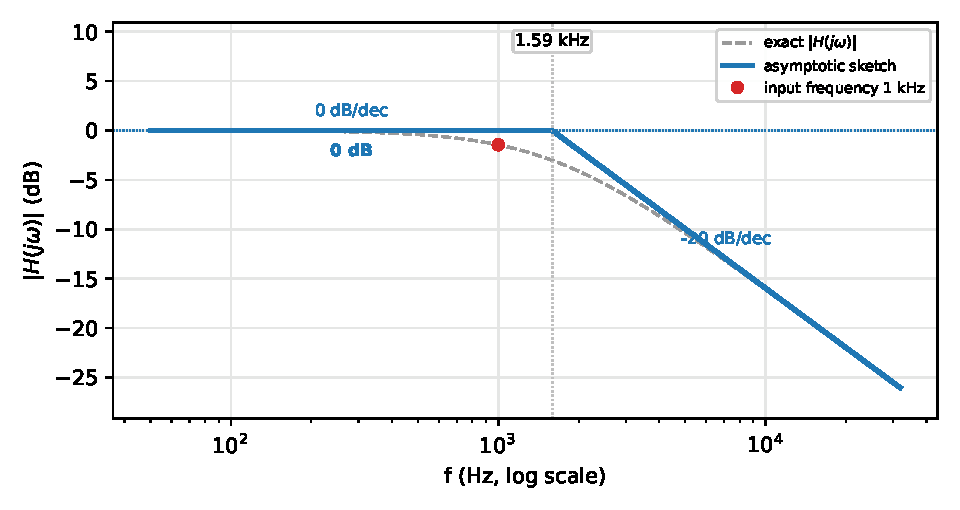
\includegraphics[width=0.78\linewidth,height=6.5cm,keepaspectratio]{p01_bode}\end{center}

{\small Blue: the straight-line sketch you are expected to draw. Dashed grey: the exact curve (about 3\,dB below the corner of an isolated pole). Red dot: the input frequency of Step 7.}
\solstep{7}{Steady-state output}The input is $V_i(t) = 2\sin\left(2\pi\cdot 1000\,t\right)$, so $\omega_{in} = 2\pi\cdot 1000 = 6280$\,rad/s. Put $s=j\omega_{in}$ in each factor (tool T5): magnitudes multiply, angles add.
{\small Rules: $\left|\frac{s}{s+p}\right| = \frac{\omega}{\sqrt{\omega^2+p^2}}$, $\angle = \frac{\pi}{2}-\tan^{-1}\frac{\omega}{p}$;\quad $\left|\frac{1}{1+s/p}\right| = \frac{1}{\sqrt{1+(\omega/p)^2}}$, $\angle = -\tan^{-1}\frac{\omega}{p}$;\quad $\left|1+\frac{s}{z}\right| = \sqrt{1+(\omega/z)^2}$, $\angle = \tan^{-1}\frac{\omega}{z}$;\quad a negative $K$ adds $-\pi$.}
\begin{center}\renewcommand{\arraystretch}{1.35}
\begin{tabular}{ccc}
\toprule
factor & magnitude & angle (rad) \\
\midrule
$1$ & $1$ & $0$ \\
$\rule[-1.7em]{0pt}{4em}\dfrac{1}{1+\dfrac{s}{2\pi\cdot 1.59\mathrm{k}}}$ & $0.8467$ & $-0.561$ \\
\textbf{total} & $\mathbf{0.8467}$ (product) & $\mathbf{-0.561}$ (sum) \\
\bottomrule
\end{tabular}\end{center}

\begin{align*}
|H(j\omega_{in})| &= 0.847, \qquad \angle H(j\omega_{in}) = -0.561\ \mathrm{rad} \\
v_{o,ac}(t) &= 0.847\times 2\,\sin\left(2\pi\cdot 1000\,t - 0.561\right) = 1.69\,\sin\left(2\pi\cdot 1000\,t - 0.561\right)
\end{align*}

\[
\boxed{V_o(t) = 1.69\,\sin\left(2\pi\cdot 1000\,t - 0.561\right)\ \mathrm{V}}
\]

\begin{ansbox}
$H(s) = 1\,\dfrac{1}{1+\dfrac{s}{2\pi\cdot 1.59\mathrm{k}}}$\quad (corners: 1.59 kHz)\\[4pt]
$V_o(t) = 1.69\,\sin\left(2\pi\cdot 1000\,t - 0.561\right)\ \mathrm{V}$
\end{ansbox}

\newpage
\subsection*{Solution 1A.2 \hfill Easy}
\begin{center}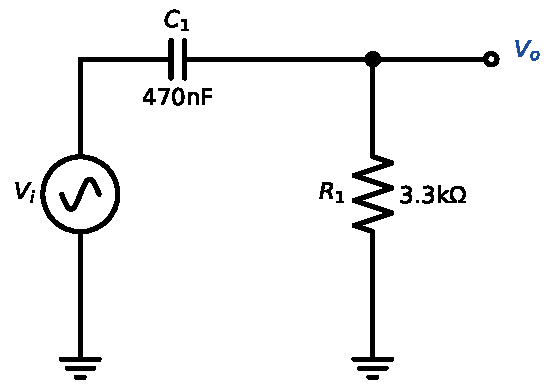
\includegraphics[width=0.8\linewidth,height=4.5cm,keepaspectratio]{p02_circuit}\end{center}
\solstep{1}{Identify the sources}Independent sources: the AC input $V_i(t)$. There is no DC source, so $V_{o,dc}=0$ and $V_o(t)=v_{o,ac}(t)$: Step 2 is skipped.
\solstep{2}{DC circuit}No DC sources: $V_{o,dc}=0$.
\solstep{3}{AC circuit}Replace every capacitor by $\frac{1}{sC}$ and every inductor by $sL$.
AC equivalent circuit (nodes named for the next step):
\begin{center}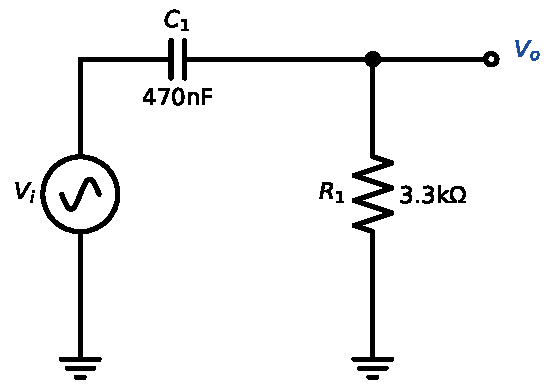
\includegraphics[width=0.95\linewidth,height=5.2cm,keepaspectratio]{p02_ac}\end{center}

\solstep{4}{Transfer function by a chain of dividers}Walk from the input to the output through the named nodes: $V_{i} \to V_{o}$. There is a single link, so $H(s)$ is just one voltage divider (tool T2).
Now each link. {\small (Algebra tip: to simplify a fraction that contains fractions, multiply its top and bottom by every inner denominator; then divide top and bottom by the leading coefficient of the denominator so that it starts with a plain $s^n$.)}
\begin{align*}
\frac{V_{o}}{V_{i}} &= \frac{R_{1}}{\frac{1}{sC_{1}} + R_{1}} = \dfrac{s}{s + 645}
\end{align*}

So:\[
H(s) = \dfrac{s}{s + 645}
\]

\solstep{5}{Standard (Bode-ready) form}Find the roots. Every root $s=-p$ of the denominator is a \emph{pole}, every root $s=-z$ of the numerator is a \emph{zero}; $|p|$ and $|z|$ are the corner frequencies (rad/s).
\begin{itemize}[leftmargin=*,itemsep=2pt]
\item Numerator: it has the factor $s$ $\Rightarrow$ 1 zero at $s=0$.
\item Denominator: $s + 645$; $s + 645 = 0 \Rightarrow s = -645$.
\end{itemize}

Factored form (leading coefficient in front):
\[
H(s) = 1\,\dfrac{s}{(s+645)}
\]

Bode-ready form: rewrite every $(s+p) = p\left(1+\frac{s}{p}\right)$ and $(s+z) = z\left(1+\frac{s}{z}\right)$, and collect all constants into $K$. Each $s$ in the numerator is paired with one of the \emph{lowest} poles as $\frac{s}{s+p}$ (that factor is $\approx 1$ above $p$). Then every factor except $K$ is $\approx 1$ inside the pass-band:
\[
H(s) = 1\,\dfrac{s}{s+2\pi\cdot 103},\qquad K = 1
\]

\begin{center}\renewcommand{\arraystretch}{1.35}
\begin{tabular}{cccc}
\toprule
type & $\omega_c$ (rad/s) & $f_c=\omega_c/2\pi$ & slope change \\
\midrule
pole & $645$ & 103 Hz & $-20$ dB/dec \\
\bottomrule
\end{tabular}\end{center}

\solstep{6}{Magnitude Bode plot}Below every corner $|H(s)|\approx 0.00155\,s$, so the plot starts with a slope of $+20$\,dB/dec. Then, moving right, each pole bends the line down by 20\,dB/dec and each zero bends it up by 20\,dB/dec (tool T6):
\begin{center}\renewcommand{\arraystretch}{1.35}
\begin{tabular}{lcl}
\toprule
frequency range & slope & asymptote level \\
\midrule
$f<$ 103 Hz & $+20$ dB/dec & 0 dB at end \\
$f>$ 103 Hz & $0$ dB/dec (flat) & 0 dB at start \\
\bottomrule
\end{tabular}\end{center}

The flat (pass-band) level is $20\log_{10}|K| = 20\log_{10}1 = 0$\,dB.
\begin{center}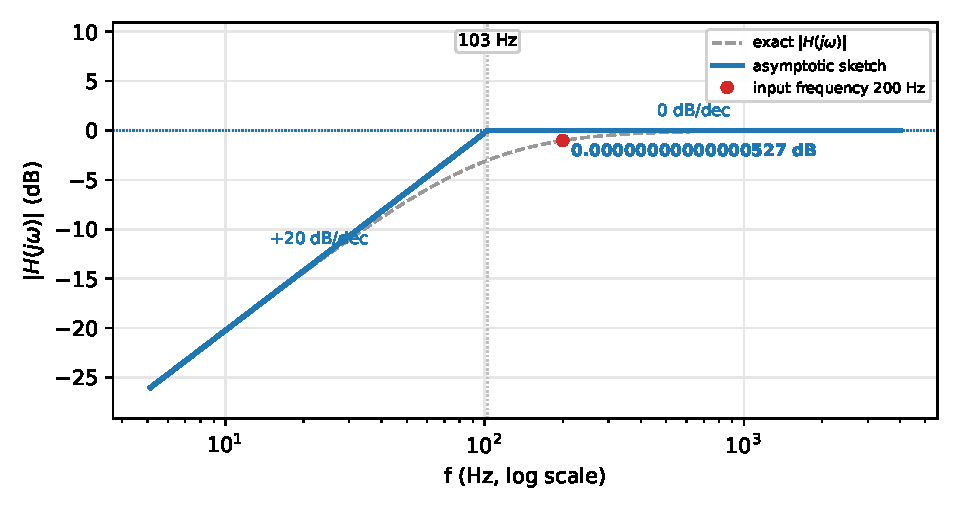
\includegraphics[width=0.78\linewidth,height=6.5cm,keepaspectratio]{p02_bode}\end{center}

{\small Blue: the straight-line sketch you are expected to draw. Dashed grey: the exact curve (about 3\,dB below the corner of an isolated pole). Red dot: the input frequency of Step 7.}
\solstep{7}{Steady-state output}The input is $V_i(t) = 1\sin\left(2\pi\cdot 200\,t\right)$, so $\omega_{in} = 2\pi\cdot 200 = 1260$\,rad/s. Put $s=j\omega_{in}$ in each factor (tool T5): magnitudes multiply, angles add.
{\small Rules: $\left|\frac{s}{s+p}\right| = \frac{\omega}{\sqrt{\omega^2+p^2}}$, $\angle = \frac{\pi}{2}-\tan^{-1}\frac{\omega}{p}$;\quad $\left|\frac{1}{1+s/p}\right| = \frac{1}{\sqrt{1+(\omega/p)^2}}$, $\angle = -\tan^{-1}\frac{\omega}{p}$;\quad $\left|1+\frac{s}{z}\right| = \sqrt{1+(\omega/z)^2}$, $\angle = \tan^{-1}\frac{\omega}{z}$;\quad a negative $K$ adds $-\pi$.}
\begin{center}\renewcommand{\arraystretch}{1.35}
\begin{tabular}{ccc}
\toprule
factor & magnitude & angle (rad) \\
\midrule
$1$ & $1$ & $0$ \\
$\rule[-1.1em]{0pt}{2.8em}\dfrac{s}{s+2\pi\cdot 103}$ & $0.8897$ & $0.474$ \\
\textbf{total} & $\mathbf{0.8897}$ (product) & $\mathbf{0.474}$ (sum) \\
\bottomrule
\end{tabular}\end{center}

\begin{align*}
|H(j\omega_{in})| &= 0.89, \qquad \angle H(j\omega_{in}) = 0.474\ \mathrm{rad} \\
v_{o,ac}(t) &= 0.89\times 1\,\sin\left(2\pi\cdot 200\,t + 0.474\right) = 0.89\,\sin\left(2\pi\cdot 200\,t + 0.474\right)
\end{align*}

\[
\boxed{V_o(t) = 0.89\,\sin\left(2\pi\cdot 200\,t + 0.474\right)\ \mathrm{V}}
\]

\begin{ansbox}
$H(s) = 1\,\dfrac{s}{s+2\pi\cdot 103}$\quad (corners: 103 Hz)\\[4pt]
$V_o(t) = 0.89\,\sin\left(2\pi\cdot 200\,t + 0.474\right)\ \mathrm{V}$
\end{ansbox}

\newpage
\subsection*{Solution 1A.3 \hfill Easy}
\begin{center}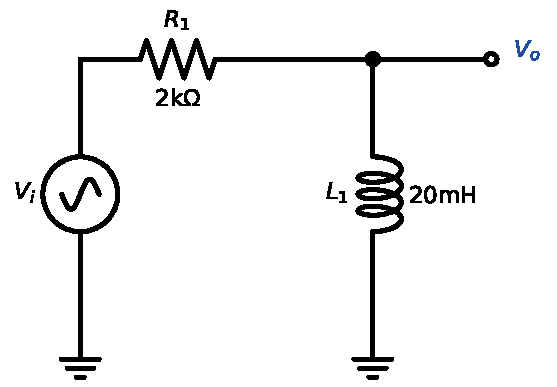
\includegraphics[width=0.8\linewidth,height=4.5cm,keepaspectratio]{p03_circuit}\end{center}
\solstep{1}{Identify the sources}Independent sources: the AC input $V_i(t)$. There is no DC source, so $V_{o,dc}=0$ and $V_o(t)=v_{o,ac}(t)$: Step 2 is skipped.
\solstep{2}{DC circuit}No DC sources: $V_{o,dc}=0$.
\solstep{3}{AC circuit}Replace every capacitor by $\frac{1}{sC}$ and every inductor by $sL$.
AC equivalent circuit (nodes named for the next step):
\begin{center}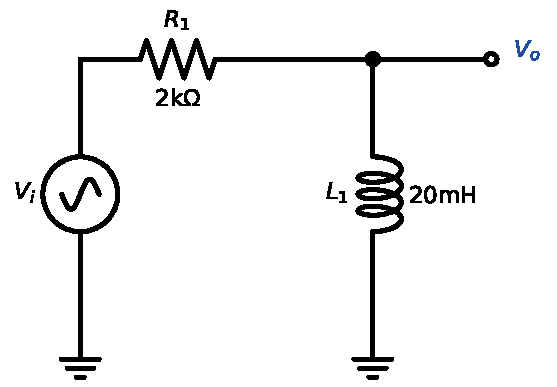
\includegraphics[width=0.95\linewidth,height=5.2cm,keepaspectratio]{p03_ac}\end{center}

\solstep{4}{Transfer function by a chain of dividers}Walk from the input to the output through the named nodes: $V_{i} \to V_{o}$. There is a single link, so $H(s)$ is just one voltage divider (tool T2).
Now each link. {\small (Algebra tip: to simplify a fraction that contains fractions, multiply its top and bottom by every inner denominator; then divide top and bottom by the leading coefficient of the denominator so that it starts with a plain $s^n$.)}
\begin{align*}
\frac{V_{o}}{V_{i}} &= \frac{sL_{1}}{R_{1} + sL_{1}} = \dfrac{s}{s + 10^{5}}
\end{align*}

So:\[
H(s) = \dfrac{s}{s + 10^{5}}
\]

\solstep{5}{Standard (Bode-ready) form}Find the roots. Every root $s=-p$ of the denominator is a \emph{pole}, every root $s=-z$ of the numerator is a \emph{zero}; $|p|$ and $|z|$ are the corner frequencies (rad/s).
\begin{itemize}[leftmargin=*,itemsep=2pt]
\item Numerator: it has the factor $s$ $\Rightarrow$ 1 zero at $s=0$.
\item Denominator: $s + 10^{5}$; $s + 10^{5} = 0 \Rightarrow s = -10^{5}$.
\end{itemize}

Factored form (leading coefficient in front):
\[
H(s) = 1\,\dfrac{s}{(s+10^{5})}
\]

Bode-ready form: rewrite every $(s+p) = p\left(1+\frac{s}{p}\right)$ and $(s+z) = z\left(1+\frac{s}{z}\right)$, and collect all constants into $K$. Each $s$ in the numerator is paired with one of the \emph{lowest} poles as $\frac{s}{s+p}$ (that factor is $\approx 1$ above $p$). Then every factor except $K$ is $\approx 1$ inside the pass-band:
\[
H(s) = 1\,\dfrac{s}{s+2\pi\cdot 15.9\mathrm{k}},\qquad K = 1
\]

\begin{center}\renewcommand{\arraystretch}{1.35}
\begin{tabular}{cccc}
\toprule
type & $\omega_c$ (rad/s) & $f_c=\omega_c/2\pi$ & slope change \\
\midrule
pole & $10^{5}$ & 15.9 kHz & $-20$ dB/dec \\
\bottomrule
\end{tabular}\end{center}

\solstep{6}{Magnitude Bode plot}Below every corner $|H(s)|\approx 10^{-5}\,s$, so the plot starts with a slope of $+20$\,dB/dec. Then, moving right, each pole bends the line down by 20\,dB/dec and each zero bends it up by 20\,dB/dec (tool T6):
\begin{center}\renewcommand{\arraystretch}{1.35}
\begin{tabular}{lcl}
\toprule
frequency range & slope & asymptote level \\
\midrule
$f<$ 15.9 kHz & $+20$ dB/dec & 0 dB at end \\
$f>$ 15.9 kHz & $0$ dB/dec (flat) & 0 dB at start \\
\bottomrule
\end{tabular}\end{center}

The flat (pass-band) level is $20\log_{10}|K| = 20\log_{10}1 = 0$\,dB.
\begin{center}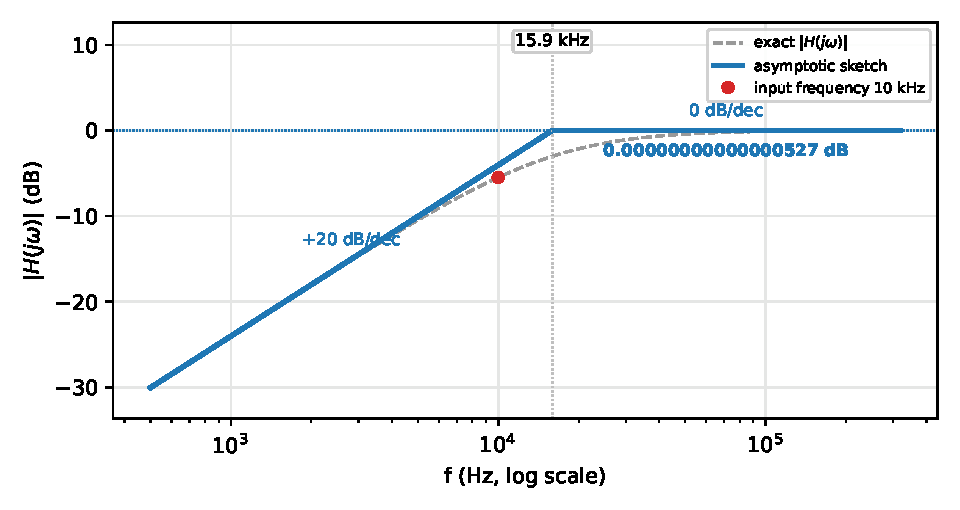
\includegraphics[width=0.78\linewidth,height=6.5cm,keepaspectratio]{p03_bode}\end{center}

{\small Blue: the straight-line sketch you are expected to draw. Dashed grey: the exact curve (about 3\,dB below the corner of an isolated pole). Red dot: the input frequency of Step 7.}
\solstep{7}{Steady-state output}The input is $V_i(t) = 0.5\sin\left(2\pi\cdot 10000\,t\right)$, so $\omega_{in} = 2\pi\cdot 10000 = 62800$\,rad/s. Put $s=j\omega_{in}$ in each factor (tool T5): magnitudes multiply, angles add.
{\small Rules: $\left|\frac{s}{s+p}\right| = \frac{\omega}{\sqrt{\omega^2+p^2}}$, $\angle = \frac{\pi}{2}-\tan^{-1}\frac{\omega}{p}$;\quad $\left|\frac{1}{1+s/p}\right| = \frac{1}{\sqrt{1+(\omega/p)^2}}$, $\angle = -\tan^{-1}\frac{\omega}{p}$;\quad $\left|1+\frac{s}{z}\right| = \sqrt{1+(\omega/z)^2}$, $\angle = \tan^{-1}\frac{\omega}{z}$;\quad a negative $K$ adds $-\pi$.}
\begin{center}\renewcommand{\arraystretch}{1.35}
\begin{tabular}{ccc}
\toprule
factor & magnitude & angle (rad) \\
\midrule
$1$ & $1$ & $0$ \\
$\rule[-1.1em]{0pt}{2.8em}\dfrac{s}{s+2\pi\cdot 15.9\mathrm{k}}$ & $0.532$ & $1.01$ \\
\textbf{total} & $\mathbf{0.532}$ (product) & $\mathbf{1.01}$ (sum) \\
\bottomrule
\end{tabular}\end{center}

\begin{align*}
|H(j\omega_{in})| &= 0.532, \qquad \angle H(j\omega_{in}) = 1.01\ \mathrm{rad} \\
v_{o,ac}(t) &= 0.532\times 0.5\,\sin\left(2\pi\cdot 10000\,t + 1.01\right) = 0.266\,\sin\left(2\pi\cdot 10000\,t + 1.01\right)
\end{align*}

\[
\boxed{V_o(t) = 0.266\,\sin\left(2\pi\cdot 10000\,t + 1.01\right)\ \mathrm{V}}
\]

\begin{ansbox}
$H(s) = 1\,\dfrac{s}{s+2\pi\cdot 15.9\mathrm{k}}$\quad (corners: 15.9 kHz)\\[4pt]
$V_o(t) = 0.266\,\sin\left(2\pi\cdot 10000\,t + 1.01\right)\ \mathrm{V}$
\end{ansbox}

\newpage
\subsection*{Solution 1A.4 \hfill Easy}
\begin{center}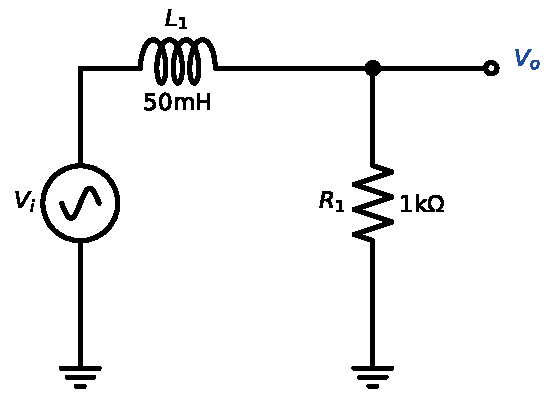
\includegraphics[width=0.8\linewidth,height=4.5cm,keepaspectratio]{p04_circuit}\end{center}
\solstep{1}{Identify the sources}Independent sources: the AC input $V_i(t)$. There is no DC source, so $V_{o,dc}=0$ and $V_o(t)=v_{o,ac}(t)$: Step 2 is skipped.
\solstep{2}{DC circuit}No DC sources: $V_{o,dc}=0$.
\solstep{3}{AC circuit}Replace every capacitor by $\frac{1}{sC}$ and every inductor by $sL$.
AC equivalent circuit (nodes named for the next step):
\begin{center}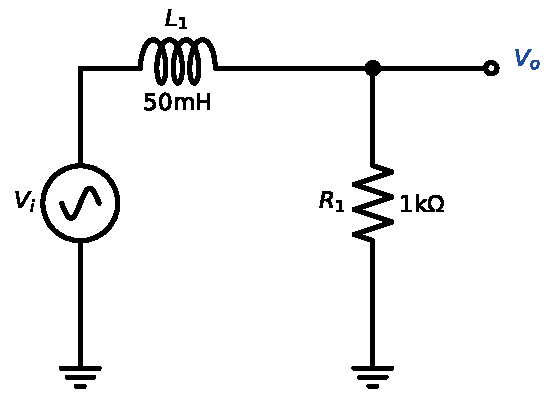
\includegraphics[width=0.95\linewidth,height=5.2cm,keepaspectratio]{p04_ac}\end{center}

\solstep{4}{Transfer function by a chain of dividers}Walk from the input to the output through the named nodes: $V_{i} \to V_{o}$. There is a single link, so $H(s)$ is just one voltage divider (tool T2).
Now each link. {\small (Algebra tip: to simplify a fraction that contains fractions, multiply its top and bottom by every inner denominator; then divide top and bottom by the leading coefficient of the denominator so that it starts with a plain $s^n$.)}
\begin{align*}
\frac{V_{o}}{V_{i}} &= \frac{R_{1}}{sL_{1} + R_{1}} = \dfrac{20000}{s + 20000}
\end{align*}

So:\[
H(s) = \dfrac{20000}{s + 20000}
\]

\solstep{5}{Standard (Bode-ready) form}Find the roots. Every root $s=-p$ of the denominator is a \emph{pole}, every root $s=-z$ of the numerator is a \emph{zero}; $|p|$ and $|z|$ are the corner frequencies (rad/s).
\begin{itemize}[leftmargin=*,itemsep=2pt]
\item Denominator: $s + 20000$; $s + 20000 = 0 \Rightarrow s = -20000$.
\end{itemize}

Factored form (leading coefficient in front):
\[
H(s) = 20000\,\dfrac{1}{(s+20000)}
\]

Bode-ready form: rewrite every $(s+p) = p\left(1+\frac{s}{p}\right)$ and $(s+z) = z\left(1+\frac{s}{z}\right)$, and collect all constants into $K$. Then every factor except $K$ is $\approx 1$ inside the pass-band:
\[
H(s) = 1\,\dfrac{1}{1+\dfrac{s}{2\pi\cdot 3.18\mathrm{k}}},\qquad K = 1
\]

\begin{center}\renewcommand{\arraystretch}{1.35}
\begin{tabular}{cccc}
\toprule
type & $\omega_c$ (rad/s) & $f_c=\omega_c/2\pi$ & slope change \\
\midrule
pole & $20000$ & 3.18 kHz & $-20$ dB/dec \\
\bottomrule
\end{tabular}\end{center}

\solstep{6}{Magnitude Bode plot}Below every corner, all factors are $\approx$ constant: $|H| \approx 1$ $= 0$\,dB (flat, 0 dB/dec). Then, moving right, each pole bends the line down by 20\,dB/dec and each zero bends it up by 20\,dB/dec (tool T6):
\begin{center}\renewcommand{\arraystretch}{1.35}
\begin{tabular}{lcl}
\toprule
frequency range & slope & asymptote level \\
\midrule
$f<$ 3.18 kHz & $0$ dB/dec (flat) & 0 dB at end \\
$f>$ 3.18 kHz & $-20$ dB/dec & 0 dB at start \\
\bottomrule
\end{tabular}\end{center}

The flat (pass-band) level is $20\log_{10}|K| = 20\log_{10}1 = 0$\,dB.
\begin{center}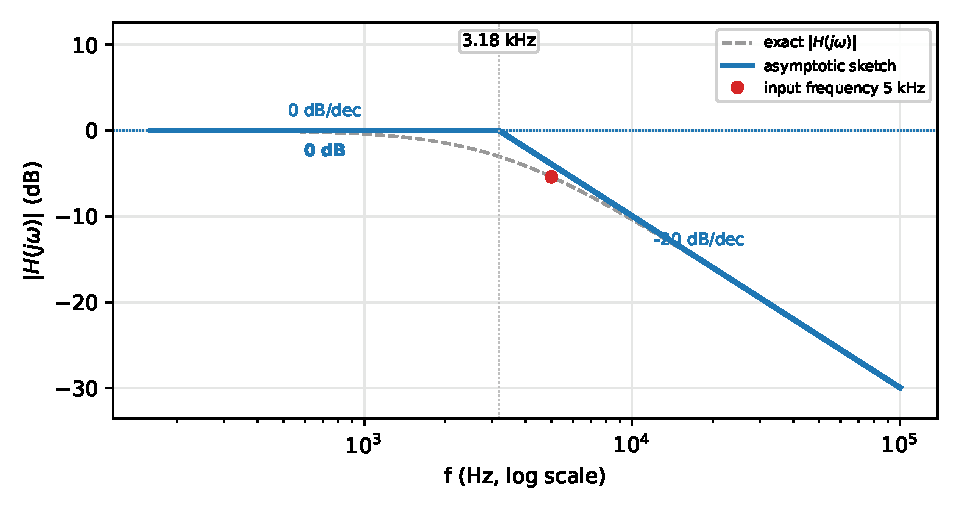
\includegraphics[width=0.78\linewidth,height=6.5cm,keepaspectratio]{p04_bode}\end{center}

{\small Blue: the straight-line sketch you are expected to draw. Dashed grey: the exact curve (about 3\,dB below the corner of an isolated pole). Red dot: the input frequency of Step 7.}
\solstep{7}{Steady-state output}The input is $V_i(t) = 3\cos\left(2\pi\cdot 5000\,t\right)$, so $\omega_{in} = 2\pi\cdot 5000 = 31400$\,rad/s. Put $s=j\omega_{in}$ in each factor (tool T5): magnitudes multiply, angles add.
{\small Rules: $\left|\frac{s}{s+p}\right| = \frac{\omega}{\sqrt{\omega^2+p^2}}$, $\angle = \frac{\pi}{2}-\tan^{-1}\frac{\omega}{p}$;\quad $\left|\frac{1}{1+s/p}\right| = \frac{1}{\sqrt{1+(\omega/p)^2}}$, $\angle = -\tan^{-1}\frac{\omega}{p}$;\quad $\left|1+\frac{s}{z}\right| = \sqrt{1+(\omega/z)^2}$, $\angle = \tan^{-1}\frac{\omega}{z}$;\quad a negative $K$ adds $-\pi$.}
\begin{center}\renewcommand{\arraystretch}{1.35}
\begin{tabular}{ccc}
\toprule
factor & magnitude & angle (rad) \\
\midrule
$1$ & $1$ & $0$ \\
$\rule[-1.7em]{0pt}{4em}\dfrac{1}{1+\dfrac{s}{2\pi\cdot 3.18\mathrm{k}}}$ & $0.537$ & $-1$ \\
\textbf{total} & $\mathbf{0.537}$ (product) & $\mathbf{-1}$ (sum) \\
\bottomrule
\end{tabular}\end{center}

\begin{align*}
|H(j\omega_{in})| &= 0.537, \qquad \angle H(j\omega_{in}) = -1\ \mathrm{rad} \\
v_{o,ac}(t) &= 0.537\times 3\,\cos\left(2\pi\cdot 5000\,t - 1\right) = 1.61\,\cos\left(2\pi\cdot 5000\,t - 1\right)
\end{align*}

\[
\boxed{V_o(t) = 1.61\,\cos\left(2\pi\cdot 5000\,t - 1\right)\ \mathrm{V}}
\]

\begin{ansbox}
$H(s) = 1\,\dfrac{1}{1+\dfrac{s}{2\pi\cdot 3.18\mathrm{k}}}$\quad (corners: 3.18 kHz)\\[4pt]
$V_o(t) = 1.61\,\cos\left(2\pi\cdot 5000\,t - 1\right)\ \mathrm{V}$
\end{ansbox}

\newpage
\subsection*{Solution 1A.5 \hfill Easy}
\begin{center}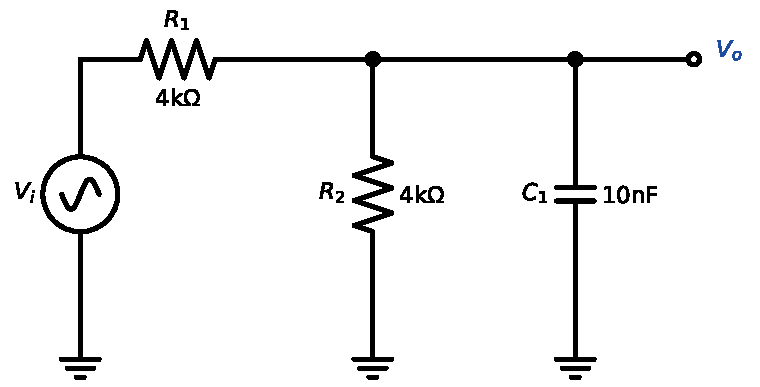
\includegraphics[width=0.8\linewidth,height=4.5cm,keepaspectratio]{p05_circuit}\end{center}
\solstep{1}{Identify the sources}Independent sources: the AC input $V_i(t)$. There is no DC source, so $V_{o,dc}=0$ and $V_o(t)=v_{o,ac}(t)$: Step 2 is skipped.
\solstep{2}{DC circuit}No DC sources: $V_{o,dc}=0$.
\solstep{3}{AC circuit}Replace every capacitor by $\frac{1}{sC}$ and every inductor by $sL$.
AC equivalent circuit (nodes named for the next step):
\begin{center}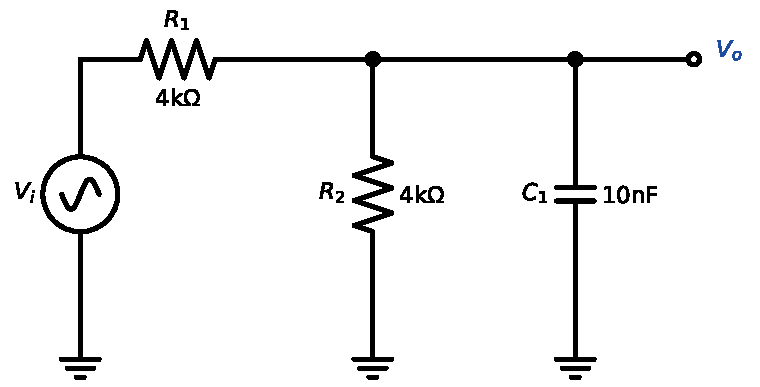
\includegraphics[width=0.95\linewidth,height=5.2cm,keepaspectratio]{p05_ac}\end{center}

\solstep{4}{Transfer function by a chain of dividers}Walk from the input to the output through the named nodes: $V_{i} \to V_{o}$. There is a single link, so $H(s)$ is just one voltage divider (tool T2).
Impedances seen \emph{looking right} from a node (everything from that node to ground, excluding what is on its left). Compute them from the far right toward the input:
\begin{align*}
Z_{o} &= R_{2} \parallel \frac{1}{sC_{1}} = \dfrac{10^{8}}{s + 25000}
\end{align*}

Now each link. {\small (Algebra tip: to simplify a fraction that contains fractions, multiply its top and bottom by every inner denominator; then divide top and bottom by the leading coefficient of the denominator so that it starts with a plain $s^n$.)}
\begin{align*}
\frac{V_{o}}{V_{i}} &= \frac{Z_{o}}{R_{1} + Z_{o}} = \dfrac{25000}{s + 50000}
\end{align*}

So:\[
H(s) = \dfrac{25000}{s + 50000}
\]

\solstep{5}{Standard (Bode-ready) form}Find the roots. Every root $s=-p$ of the denominator is a \emph{pole}, every root $s=-z$ of the numerator is a \emph{zero}; $|p|$ and $|z|$ are the corner frequencies (rad/s).
\begin{itemize}[leftmargin=*,itemsep=2pt]
\item Denominator: $s + 50000$; $s + 50000 = 0 \Rightarrow s = -50000$.
\end{itemize}

Factored form (leading coefficient in front):
\[
H(s) = 25000\,\dfrac{1}{(s+50000)}
\]

Bode-ready form: rewrite every $(s+p) = p\left(1+\frac{s}{p}\right)$ and $(s+z) = z\left(1+\frac{s}{z}\right)$, and collect all constants into $K$. Then every factor except $K$ is $\approx 1$ inside the pass-band:
\[
H(s) = 0.5\,\dfrac{1}{1+\dfrac{s}{2\pi\cdot 7.96\mathrm{k}}},\qquad K = 0.5
\]

\begin{center}\renewcommand{\arraystretch}{1.35}
\begin{tabular}{cccc}
\toprule
type & $\omega_c$ (rad/s) & $f_c=\omega_c/2\pi$ & slope change \\
\midrule
pole & $50000$ & 7.96 kHz & $-20$ dB/dec \\
\bottomrule
\end{tabular}\end{center}

\solstep{6}{Magnitude Bode plot}Below every corner, all factors are $\approx$ constant: $|H| \approx 0.5$ $= -6.02$\,dB (flat, 0 dB/dec). Then, moving right, each pole bends the line down by 20\,dB/dec and each zero bends it up by 20\,dB/dec (tool T6):
\begin{center}\renewcommand{\arraystretch}{1.35}
\begin{tabular}{lcl}
\toprule
frequency range & slope & asymptote level \\
\midrule
$f<$ 7.96 kHz & $0$ dB/dec (flat) & -6.02 dB at end \\
$f>$ 7.96 kHz & $-20$ dB/dec & -6.02 dB at start \\
\bottomrule
\end{tabular}\end{center}

The flat (pass-band) level is $20\log_{10}|K| = 20\log_{10}0.5 = -6.02$\,dB.
\begin{center}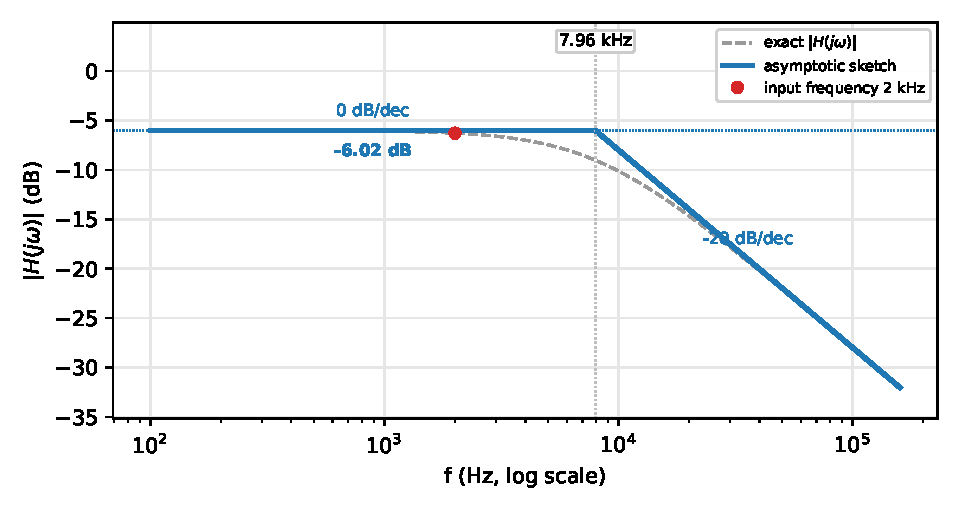
\includegraphics[width=0.78\linewidth,height=6.5cm,keepaspectratio]{p05_bode}\end{center}

{\small Blue: the straight-line sketch you are expected to draw. Dashed grey: the exact curve (about 3\,dB below the corner of an isolated pole). Red dot: the input frequency of Step 7.}
\solstep{7}{Steady-state output}The input is $V_i(t) = 1\sin\left(2\pi\cdot 2000\,t\right)$, so $\omega_{in} = 2\pi\cdot 2000 = 12600$\,rad/s. Put $s=j\omega_{in}$ in each factor (tool T5): magnitudes multiply, angles add.
{\small Rules: $\left|\frac{s}{s+p}\right| = \frac{\omega}{\sqrt{\omega^2+p^2}}$, $\angle = \frac{\pi}{2}-\tan^{-1}\frac{\omega}{p}$;\quad $\left|\frac{1}{1+s/p}\right| = \frac{1}{\sqrt{1+(\omega/p)^2}}$, $\angle = -\tan^{-1}\frac{\omega}{p}$;\quad $\left|1+\frac{s}{z}\right| = \sqrt{1+(\omega/z)^2}$, $\angle = \tan^{-1}\frac{\omega}{z}$;\quad a negative $K$ adds $-\pi$.}
\begin{center}\renewcommand{\arraystretch}{1.35}
\begin{tabular}{ccc}
\toprule
factor & magnitude & angle (rad) \\
\midrule
$0.5$ & $0.5$ & $0$ \\
$\rule[-1.7em]{0pt}{4em}\dfrac{1}{1+\dfrac{s}{2\pi\cdot 7.96\mathrm{k}}}$ & $0.9698$ & $-0.246$ \\
\textbf{total} & $\mathbf{0.4849}$ (product) & $\mathbf{-0.246}$ (sum) \\
\bottomrule
\end{tabular}\end{center}

\begin{align*}
|H(j\omega_{in})| &= 0.485, \qquad \angle H(j\omega_{in}) = -0.246\ \mathrm{rad} \\
v_{o,ac}(t) &= 0.485\times 1\,\sin\left(2\pi\cdot 2000\,t - 0.246\right) = 0.485\,\sin\left(2\pi\cdot 2000\,t - 0.246\right)
\end{align*}

\[
\boxed{V_o(t) = 0.485\,\sin\left(2\pi\cdot 2000\,t - 0.246\right)\ \mathrm{V}}
\]

\begin{ansbox}
$H(s) = 0.5\,\dfrac{1}{1+\dfrac{s}{2\pi\cdot 7.96\mathrm{k}}}$\quad (corners: 7.96 kHz)\\[4pt]
$V_o(t) = 0.485\,\sin\left(2\pi\cdot 2000\,t - 0.246\right)\ \mathrm{V}$
\end{ansbox}

\newpage
\subsection*{Solution 1A.6 \hfill Easy}
\begin{center}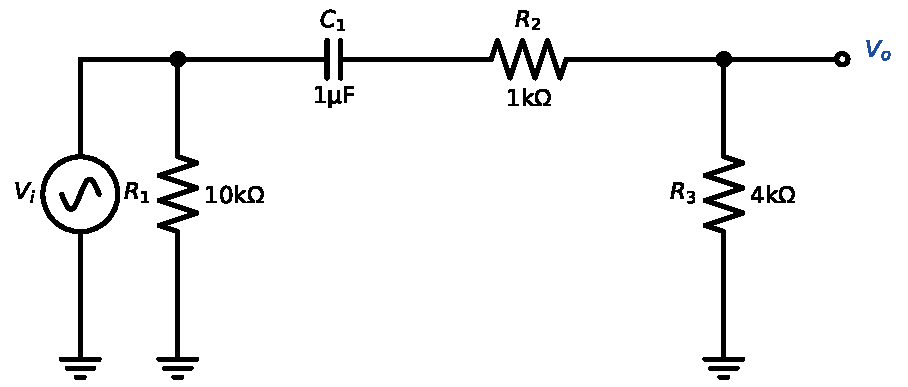
\includegraphics[width=0.8\linewidth,height=4.5cm,keepaspectratio]{p06_circuit}\end{center}
\solstep{1}{Identify the sources}Independent sources: the AC input $V_i(t)$. There is no DC source, so $V_{o,dc}=0$ and $V_o(t)=v_{o,ac}(t)$: Step 2 is skipped.
\solstep{2}{DC circuit}No DC sources: $V_{o,dc}=0$.
\solstep{3}{AC circuit}Replace every capacitor by $\frac{1}{sC}$ and every inductor by $sL$.
\begin{itemize}[leftmargin=*,itemsep=2pt]
\item $R_{1}$ sits directly across the ideal input source $V_i$. An ideal voltage source keeps its voltage whatever you connect to it, so $R_{1}$ cannot change any node voltage: it drops out of $H(s)$.
\end{itemize}

AC equivalent circuit (nodes named for the next step):
\begin{center}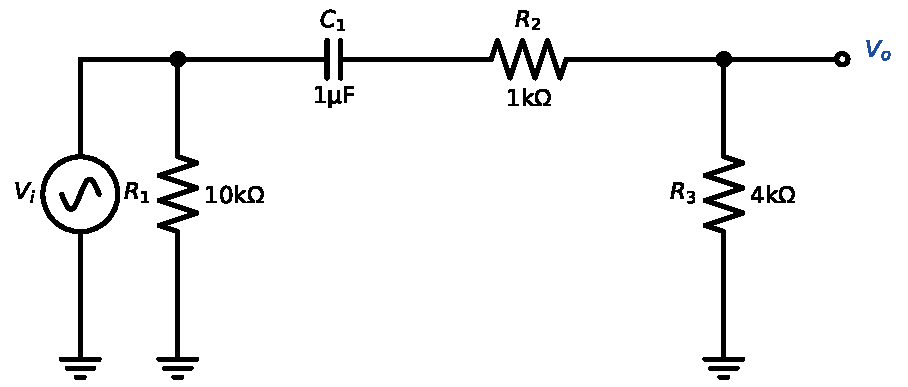
\includegraphics[width=0.95\linewidth,height=5.2cm,keepaspectratio]{p06_ac}\end{center}

\solstep{4}{Transfer function by a chain of dividers}Walk from the input to the output through the named nodes: $V_{i} \to V_{o}$. There is a single link, so $H(s)$ is just one voltage divider (tool T2).
Now each link. {\small (Algebra tip: to simplify a fraction that contains fractions, multiply its top and bottom by every inner denominator; then divide top and bottom by the leading coefficient of the denominator so that it starts with a plain $s^n$.)}
\begin{align*}
\frac{V_{o}}{V_{i}} &= \frac{R_{3}}{\frac{1}{sC_{1}} + R_{2} + R_{3}} = \dfrac{0.8\,s}{s + 200}
\end{align*}

So:\[
H(s) = \dfrac{0.8\,s}{s + 200}
\]

\solstep{5}{Standard (Bode-ready) form}Find the roots. Every root $s=-p$ of the denominator is a \emph{pole}, every root $s=-z$ of the numerator is a \emph{zero}; $|p|$ and $|z|$ are the corner frequencies (rad/s).
\begin{itemize}[leftmargin=*,itemsep=2pt]
\item Numerator: it has the factor $s$ $\Rightarrow$ 1 zero at $s=0$.
\item Denominator: $s + 200$; $s + 200 = 0 \Rightarrow s = -200$.
\end{itemize}

Factored form (leading coefficient in front):
\[
H(s) = 0.8\,\dfrac{s}{(s+200)}
\]

Bode-ready form: rewrite every $(s+p) = p\left(1+\frac{s}{p}\right)$ and $(s+z) = z\left(1+\frac{s}{z}\right)$, and collect all constants into $K$. Each $s$ in the numerator is paired with one of the \emph{lowest} poles as $\frac{s}{s+p}$ (that factor is $\approx 1$ above $p$). Then every factor except $K$ is $\approx 1$ inside the pass-band:
\[
H(s) = 0.8\,\dfrac{s}{s+2\pi\cdot 31.8},\qquad K = 0.8
\]

\begin{center}\renewcommand{\arraystretch}{1.35}
\begin{tabular}{cccc}
\toprule
type & $\omega_c$ (rad/s) & $f_c=\omega_c/2\pi$ & slope change \\
\midrule
pole & $200$ & 31.8 Hz & $-20$ dB/dec \\
\bottomrule
\end{tabular}\end{center}

\solstep{6}{Magnitude Bode plot}Below every corner $|H(s)|\approx 0.004\,s$, so the plot starts with a slope of $+20$\,dB/dec. Then, moving right, each pole bends the line down by 20\,dB/dec and each zero bends it up by 20\,dB/dec (tool T6):
\begin{center}\renewcommand{\arraystretch}{1.35}
\begin{tabular}{lcl}
\toprule
frequency range & slope & asymptote level \\
\midrule
$f<$ 31.8 Hz & $+20$ dB/dec & -1.94 dB at end \\
$f>$ 31.8 Hz & $0$ dB/dec (flat) & -1.94 dB at start \\
\bottomrule
\end{tabular}\end{center}

The flat (pass-band) level is $20\log_{10}|K| = 20\log_{10}0.8 = -1.94$\,dB.
\begin{center}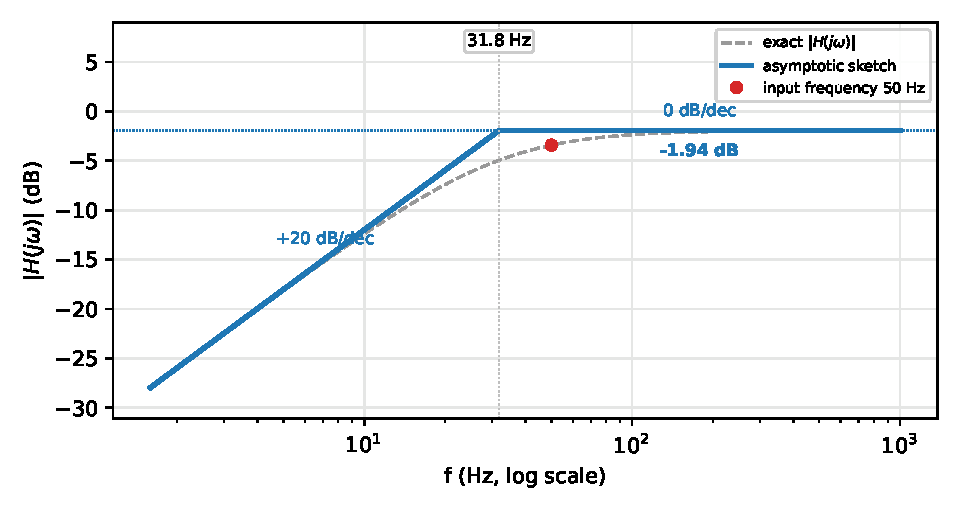
\includegraphics[width=0.78\linewidth,height=6.5cm,keepaspectratio]{p06_bode}\end{center}

{\small Blue: the straight-line sketch you are expected to draw. Dashed grey: the exact curve (about 3\,dB below the corner of an isolated pole). Red dot: the input frequency of Step 7.}
\solstep{7}{Steady-state output}The input is $V_i(t) = 0.2\sin\left(2\pi\cdot 50\,t\right)$, so $\omega_{in} = 2\pi\cdot 50 = 314$\,rad/s. Put $s=j\omega_{in}$ in each factor (tool T5): magnitudes multiply, angles add.
{\small Rules: $\left|\frac{s}{s+p}\right| = \frac{\omega}{\sqrt{\omega^2+p^2}}$, $\angle = \frac{\pi}{2}-\tan^{-1}\frac{\omega}{p}$;\quad $\left|\frac{1}{1+s/p}\right| = \frac{1}{\sqrt{1+(\omega/p)^2}}$, $\angle = -\tan^{-1}\frac{\omega}{p}$;\quad $\left|1+\frac{s}{z}\right| = \sqrt{1+(\omega/z)^2}$, $\angle = \tan^{-1}\frac{\omega}{z}$;\quad a negative $K$ adds $-\pi$.}
\begin{center}\renewcommand{\arraystretch}{1.35}
\begin{tabular}{ccc}
\toprule
factor & magnitude & angle (rad) \\
\midrule
$0.8$ & $0.8$ & $0$ \\
$\rule[-1.1em]{0pt}{2.8em}\dfrac{s}{s+2\pi\cdot 31.8}$ & $0.8436$ & $0.567$ \\
\textbf{total} & $\mathbf{0.6749}$ (product) & $\mathbf{0.567}$ (sum) \\
\bottomrule
\end{tabular}\end{center}

\begin{align*}
|H(j\omega_{in})| &= 0.675, \qquad \angle H(j\omega_{in}) = 0.567\ \mathrm{rad} \\
v_{o,ac}(t) &= 0.675\times 0.2\,\sin\left(2\pi\cdot 50\,t + 0.567\right) = 0.135\,\sin\left(2\pi\cdot 50\,t + 0.567\right)
\end{align*}

\[
\boxed{V_o(t) = 0.135\,\sin\left(2\pi\cdot 50\,t + 0.567\right)\ \mathrm{V}}
\]

\begin{ansbox}
$H(s) = 0.8\,\dfrac{s}{s+2\pi\cdot 31.8}$\quad (corners: 31.8 Hz)\\[4pt]
$V_o(t) = 0.135\,\sin\left(2\pi\cdot 50\,t + 0.567\right)\ \mathrm{V}$
\end{ansbox}

\newpage
\subsection*{Solution 1A.7 \hfill Medium}
\begin{center}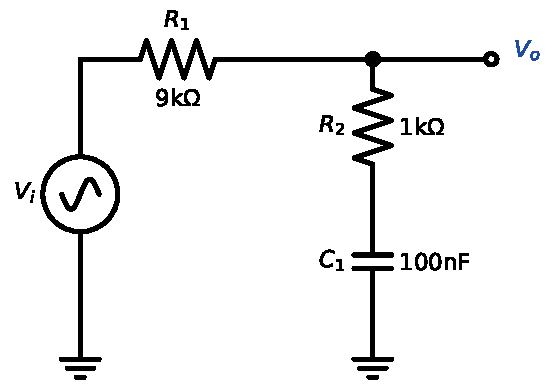
\includegraphics[width=0.8\linewidth,height=4.5cm,keepaspectratio]{p07_circuit}\end{center}
\solstep{1}{Identify the sources}Independent sources: the AC input $V_i(t)$. There is no DC source, so $V_{o,dc}=0$ and $V_o(t)=v_{o,ac}(t)$: Step 2 is skipped.
\solstep{2}{DC circuit}No DC sources: $V_{o,dc}=0$.
\solstep{3}{AC circuit}Replace every capacitor by $\frac{1}{sC}$ and every inductor by $sL$.
AC equivalent circuit (nodes named for the next step):
\begin{center}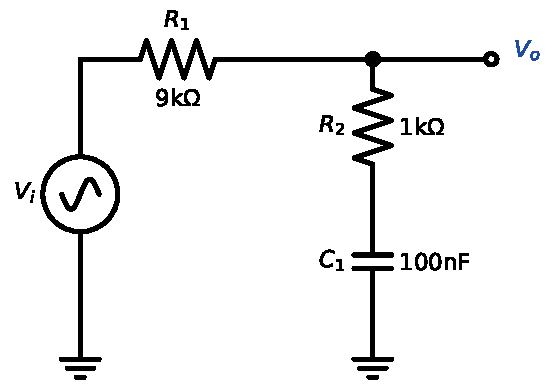
\includegraphics[width=0.95\linewidth,height=5.2cm,keepaspectratio]{p07_ac}\end{center}

\solstep{4}{Transfer function by a chain of dividers}Walk from the input to the output through the named nodes: $V_{i} \to V_{o}$. There is a single link, so $H(s)$ is just one voltage divider (tool T2).
Impedances seen \emph{looking right} from a node (everything from that node to ground, excluding what is on its left). Compute them from the far right toward the input:
\begin{align*}
Z_{o} &= R_{2} + \frac{1}{sC_{1}} = \dfrac{1000\,s + 10^{7}}{s}
\end{align*}

Now each link. {\small (Algebra tip: to simplify a fraction that contains fractions, multiply its top and bottom by every inner denominator; then divide top and bottom by the leading coefficient of the denominator so that it starts with a plain $s^n$.)}
\begin{align*}
\frac{V_{o}}{V_{i}} &= \frac{Z_{o}}{R_{1} + Z_{o}} = \dfrac{0.1\,s + 1000}{s + 1000}
\end{align*}

So:\[
H(s) = \dfrac{0.1\,s + 1000}{s + 1000}
\]

\solstep{5}{Standard (Bode-ready) form}Find the roots. Every root $s=-p$ of the denominator is a \emph{pole}, every root $s=-z$ of the numerator is a \emph{zero}; $|p|$ and $|z|$ are the corner frequencies (rad/s).
\begin{itemize}[leftmargin=*,itemsep=2pt]
\item Numerator: $0.1\,s + 1000$; divide by the leading coefficient $0.1$ (this does not move the roots): $s + 10000$; $s + 10000 = 0 \Rightarrow s = -10000$.
\item Denominator: $s + 1000$; $s + 1000 = 0 \Rightarrow s = -1000$.
\end{itemize}

Factored form (leading coefficient in front):
\[
H(s) = 0.1\,\dfrac{(s+10000)}{(s+1000)}
\]

Bode-ready form: rewrite every $(s+p) = p\left(1+\frac{s}{p}\right)$ and $(s+z) = z\left(1+\frac{s}{z}\right)$, and collect all constants into $K$. Then every factor except $K$ is $\approx 1$ inside the pass-band:
\[
H(s) = 1\,\dfrac{1}{1+\dfrac{s}{2\pi\cdot 159}}\,\left(1+\dfrac{s}{2\pi\cdot 1.59\mathrm{k}}\right),\qquad K = 1
\]

\begin{center}\renewcommand{\arraystretch}{1.35}
\begin{tabular}{cccc}
\toprule
type & $\omega_c$ (rad/s) & $f_c=\omega_c/2\pi$ & slope change \\
\midrule
pole & $1000$ & 159 Hz & $-20$ dB/dec \\
zero & $10000$ & 1.59 kHz & $+20$ dB/dec \\
\bottomrule
\end{tabular}\end{center}

\solstep{6}{Magnitude Bode plot}Below every corner, all factors are $\approx$ constant: $|H| \approx 1$ $= 0$\,dB (flat, 0 dB/dec). Then, moving right, each pole bends the line down by 20\,dB/dec and each zero bends it up by 20\,dB/dec (tool T6):
\begin{center}\renewcommand{\arraystretch}{1.35}
\begin{tabular}{lcl}
\toprule
frequency range & slope & asymptote level \\
\midrule
$f<$ 159 Hz & $0$ dB/dec (flat) & 0 dB at end \\
159 Hz -- 1.59 kHz & $-20$ dB/dec & 0 dB at start, -20 dB at end \\
$f>$ 1.59 kHz & $0$ dB/dec (flat) & -20 dB at start \\
\bottomrule
\end{tabular}\end{center}

\begin{center}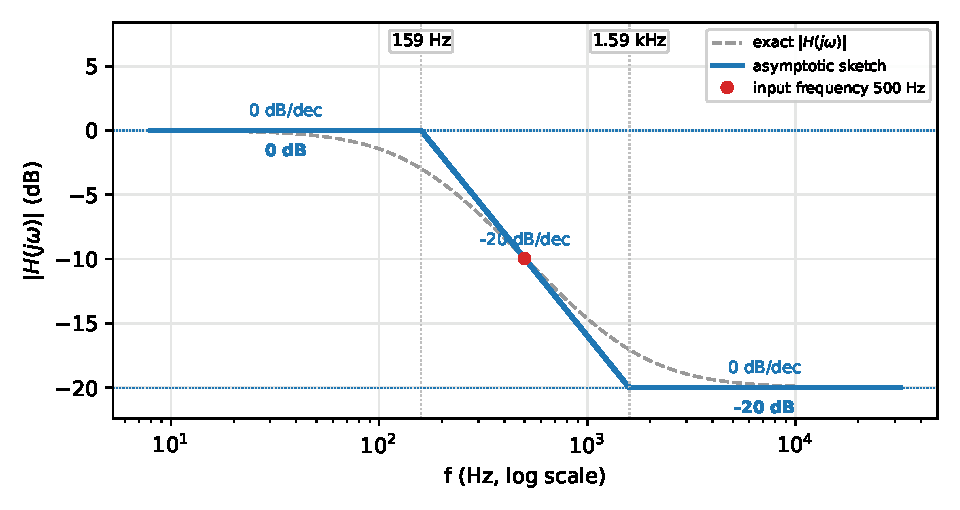
\includegraphics[width=0.78\linewidth,height=6.5cm,keepaspectratio]{p07_bode}\end{center}

{\small Blue: the straight-line sketch you are expected to draw. Dashed grey: the exact curve (about 3\,dB below the corner of an isolated pole). Red dot: the input frequency of Step 7.}
\solstep{7}{Steady-state output}The input is $V_i(t) = 1\sin\left(2\pi\cdot 500\,t\right)$, so $\omega_{in} = 2\pi\cdot 500 = 3140$\,rad/s. Put $s=j\omega_{in}$ in each factor (tool T5): magnitudes multiply, angles add.
{\small Rules: $\left|\frac{s}{s+p}\right| = \frac{\omega}{\sqrt{\omega^2+p^2}}$, $\angle = \frac{\pi}{2}-\tan^{-1}\frac{\omega}{p}$;\quad $\left|\frac{1}{1+s/p}\right| = \frac{1}{\sqrt{1+(\omega/p)^2}}$, $\angle = -\tan^{-1}\frac{\omega}{p}$;\quad $\left|1+\frac{s}{z}\right| = \sqrt{1+(\omega/z)^2}$, $\angle = \tan^{-1}\frac{\omega}{z}$;\quad a negative $K$ adds $-\pi$.}
\begin{center}\renewcommand{\arraystretch}{1.35}
\begin{tabular}{ccc}
\toprule
factor & magnitude & angle (rad) \\
\midrule
$1$ & $1$ & $0$ \\
$\rule[-1.7em]{0pt}{4em}\dfrac{1}{1+\dfrac{s}{2\pi\cdot 159}}$ & $0.3033$ & $-1.26$ \\
$\rule[-1.1em]{0pt}{2.8em}\left(1+\dfrac{s}{2\pi\cdot 1.59\mathrm{k}}\right)$ & $1.048$ & $0.304$ \\
\textbf{total} & $\mathbf{0.3179}$ (product) & $\mathbf{-0.958}$ (sum) \\
\bottomrule
\end{tabular}\end{center}

\begin{align*}
|H(j\omega_{in})| &= 0.318, \qquad \angle H(j\omega_{in}) = -0.958\ \mathrm{rad} \\
v_{o,ac}(t) &= 0.318\times 1\,\sin\left(2\pi\cdot 500\,t - 0.958\right) = 0.318\,\sin\left(2\pi\cdot 500\,t - 0.958\right)
\end{align*}

\[
\boxed{V_o(t) = 0.318\,\sin\left(2\pi\cdot 500\,t - 0.958\right)\ \mathrm{V}}
\]

\begin{ansbox}
$H(s) = 1\,\dfrac{1}{1+\dfrac{s}{2\pi\cdot 159}}\,\left(1+\dfrac{s}{2\pi\cdot 1.59\mathrm{k}}\right)$\quad (corners: 159 Hz, 1.59 kHz)\\[4pt]
$V_o(t) = 0.318\,\sin\left(2\pi\cdot 500\,t - 0.958\right)\ \mathrm{V}$
\end{ansbox}

\newpage
\subsection*{Solution 1A.8 \hfill Medium}
\begin{center}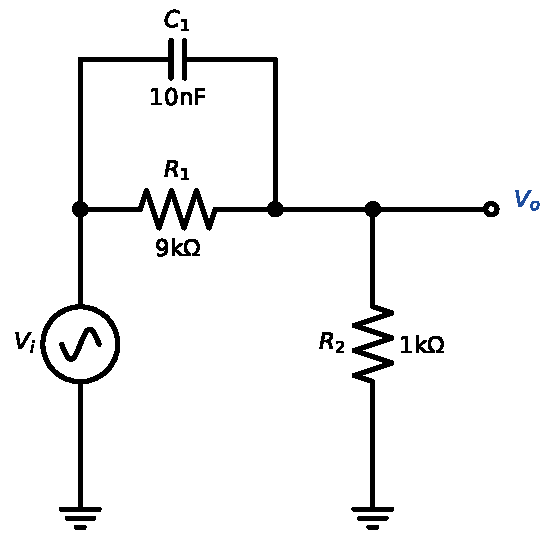
\includegraphics[width=0.8\linewidth,height=4.5cm,keepaspectratio]{p08_circuit}\end{center}
\solstep{1}{Identify the sources}Independent sources: the AC input $V_i(t)$. There is no DC source, so $V_{o,dc}=0$ and $V_o(t)=v_{o,ac}(t)$: Step 2 is skipped.
\solstep{2}{DC circuit}No DC sources: $V_{o,dc}=0$.
\solstep{3}{AC circuit}Replace every capacitor by $\frac{1}{sC}$ and every inductor by $sL$.
AC equivalent circuit (nodes named for the next step):
\begin{center}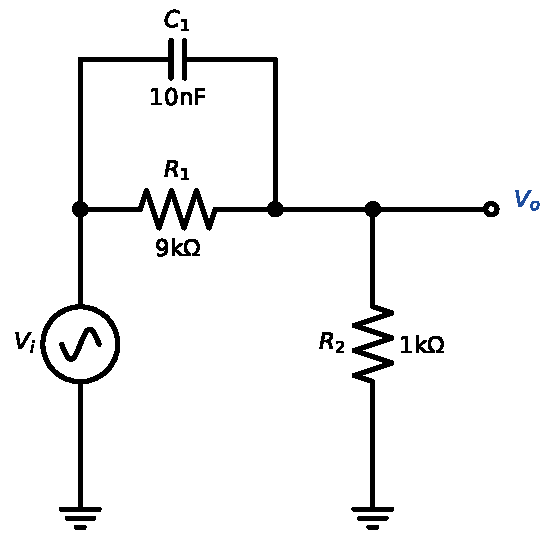
\includegraphics[width=0.95\linewidth,height=5.2cm,keepaspectratio]{p08_ac}\end{center}

\solstep{4}{Transfer function by a chain of dividers}Walk from the input to the output through the named nodes: $V_{i} \to V_{o}$. There is a single link, so $H(s)$ is just one voltage divider (tool T2).
Now each link. {\small (Algebra tip: to simplify a fraction that contains fractions, multiply its top and bottom by every inner denominator; then divide top and bottom by the leading coefficient of the denominator so that it starts with a plain $s^n$.)}
\begin{align*}
\frac{V_{o}}{V_{i}} &= \frac{R_{2}}{R_{1} \parallel \frac{1}{sC_{1}} + R_{2}} = \dfrac{s + 11100}{s + 1.11\times 10^{5}}
\end{align*}

So:\[
H(s) = \dfrac{s + 11100}{s + 1.11\times 10^{5}}
\]

\solstep{5}{Standard (Bode-ready) form}Find the roots. Every root $s=-p$ of the denominator is a \emph{pole}, every root $s=-z$ of the numerator is a \emph{zero}; $|p|$ and $|z|$ are the corner frequencies (rad/s).
\begin{itemize}[leftmargin=*,itemsep=2pt]
\item Numerator: $s + 11100$; $s + 11100 = 0 \Rightarrow s = -11100$.
\item Denominator: $s + 1.11\times 10^{5}$; $s + 1.11\times 10^{5} = 0 \Rightarrow s = -1.11\times 10^{5}$.
\end{itemize}

Factored form (leading coefficient in front):
\[
H(s) = 1\,\dfrac{(s+11100)}{(s+1.11\times 10^{5})}
\]

Bode-ready form: rewrite every $(s+p) = p\left(1+\frac{s}{p}\right)$ and $(s+z) = z\left(1+\frac{s}{z}\right)$, and collect all constants into $K$. Then every factor except $K$ is $\approx 1$ inside the pass-band:
\[
H(s) = 0.1\,\left(1+\dfrac{s}{2\pi\cdot 1.77\mathrm{k}}\right)\,\dfrac{1}{1+\dfrac{s}{2\pi\cdot 17.7\mathrm{k}}},\qquad K = 0.1
\]

\begin{center}\renewcommand{\arraystretch}{1.35}
\begin{tabular}{cccc}
\toprule
type & $\omega_c$ (rad/s) & $f_c=\omega_c/2\pi$ & slope change \\
\midrule
zero & $11100$ & 1.77 kHz & $+20$ dB/dec \\
pole & $1.11\times 10^{5}$ & 17.7 kHz & $-20$ dB/dec \\
\bottomrule
\end{tabular}\end{center}

\solstep{6}{Magnitude Bode plot}Below every corner, all factors are $\approx$ constant: $|H| \approx 0.1$ $= -20$\,dB (flat, 0 dB/dec). Then, moving right, each pole bends the line down by 20\,dB/dec and each zero bends it up by 20\,dB/dec (tool T6):
\begin{center}\renewcommand{\arraystretch}{1.35}
\begin{tabular}{lcl}
\toprule
frequency range & slope & asymptote level \\
\midrule
$f<$ 1.77 kHz & $0$ dB/dec (flat) & -20 dB at end \\
1.77 kHz -- 17.7 kHz & $+20$ dB/dec & -20 dB at start, 0 dB at end \\
$f>$ 17.7 kHz & $0$ dB/dec (flat) & 0 dB at start \\
\bottomrule
\end{tabular}\end{center}

\begin{center}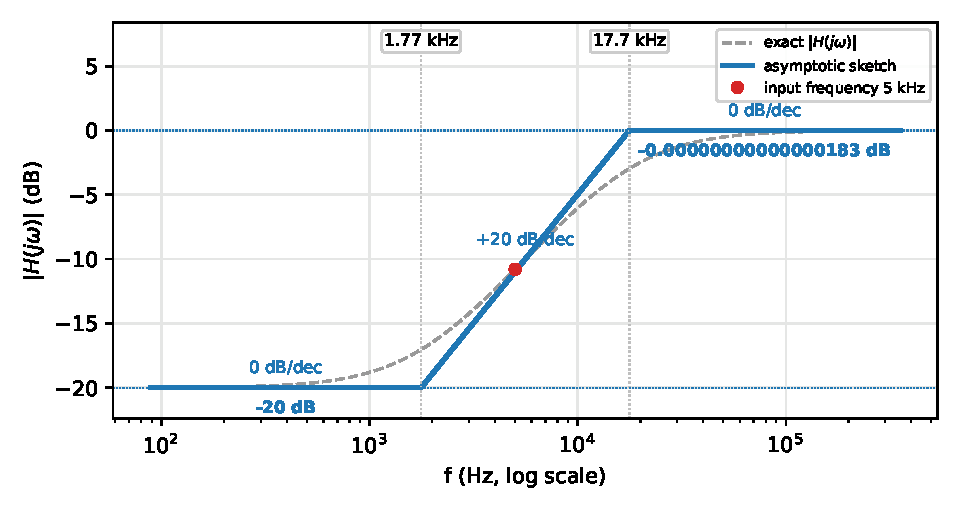
\includegraphics[width=0.78\linewidth,height=6.5cm,keepaspectratio]{p08_bode}\end{center}

{\small Blue: the straight-line sketch you are expected to draw. Dashed grey: the exact curve (about 3\,dB below the corner of an isolated pole). Red dot: the input frequency of Step 7.}
\solstep{7}{Steady-state output}The input is $V_i(t) = 0.5\sin\left(2\pi\cdot 5000\,t\right)$, so $\omega_{in} = 2\pi\cdot 5000 = 31400$\,rad/s. Put $s=j\omega_{in}$ in each factor (tool T5): magnitudes multiply, angles add.
{\small Rules: $\left|\frac{s}{s+p}\right| = \frac{\omega}{\sqrt{\omega^2+p^2}}$, $\angle = \frac{\pi}{2}-\tan^{-1}\frac{\omega}{p}$;\quad $\left|\frac{1}{1+s/p}\right| = \frac{1}{\sqrt{1+(\omega/p)^2}}$, $\angle = -\tan^{-1}\frac{\omega}{p}$;\quad $\left|1+\frac{s}{z}\right| = \sqrt{1+(\omega/z)^2}$, $\angle = \tan^{-1}\frac{\omega}{z}$;\quad a negative $K$ adds $-\pi$.}
\begin{center}\renewcommand{\arraystretch}{1.35}
\begin{tabular}{ccc}
\toprule
factor & magnitude & angle (rad) \\
\midrule
$0.1$ & $0.1$ & $0$ \\
$\rule[-1.1em]{0pt}{2.8em}\left(1+\dfrac{s}{2\pi\cdot 1.77\mathrm{k}}\right)$ & $2.999$ & $1.23$ \\
$\rule[-1.7em]{0pt}{4em}\dfrac{1}{1+\dfrac{s}{2\pi\cdot 17.7\mathrm{k}}}$ & $0.9623$ & $-0.276$ \\
\textbf{total} & $\mathbf{0.2886}$ (product) & $\mathbf{0.955}$ (sum) \\
\bottomrule
\end{tabular}\end{center}

\begin{align*}
|H(j\omega_{in})| &= 0.289, \qquad \angle H(j\omega_{in}) = 0.955\ \mathrm{rad} \\
v_{o,ac}(t) &= 0.289\times 0.5\,\sin\left(2\pi\cdot 5000\,t + 0.955\right) = 0.144\,\sin\left(2\pi\cdot 5000\,t + 0.955\right)
\end{align*}

\[
\boxed{V_o(t) = 0.144\,\sin\left(2\pi\cdot 5000\,t + 0.955\right)\ \mathrm{V}}
\]

\begin{ansbox}
$H(s) = 0.1\,\left(1+\dfrac{s}{2\pi\cdot 1.77\mathrm{k}}\right)\,\dfrac{1}{1+\dfrac{s}{2\pi\cdot 17.7\mathrm{k}}}$\quad (corners: 1.77 kHz, 17.7 kHz)\\[4pt]
$V_o(t) = 0.144\,\sin\left(2\pi\cdot 5000\,t + 0.955\right)\ \mathrm{V}$
\end{ansbox}

\newpage
\subsection*{Solution 1A.9 \hfill Medium}
\begin{center}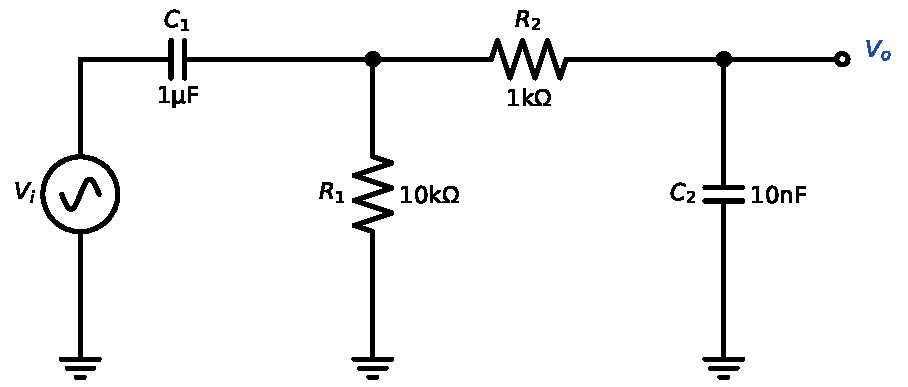
\includegraphics[width=0.8\linewidth,height=4.5cm,keepaspectratio]{p09_circuit}\end{center}
\solstep{1}{Identify the sources}Independent sources: the AC input $V_i(t)$. There is no DC source, so $V_{o,dc}=0$ and $V_o(t)=v_{o,ac}(t)$: Step 2 is skipped.
\solstep{2}{DC circuit}No DC sources: $V_{o,dc}=0$.
\solstep{3}{AC circuit}Replace every capacitor by $\frac{1}{sC}$ and every inductor by $sL$.
AC equivalent circuit (nodes named for the next step):
\begin{center}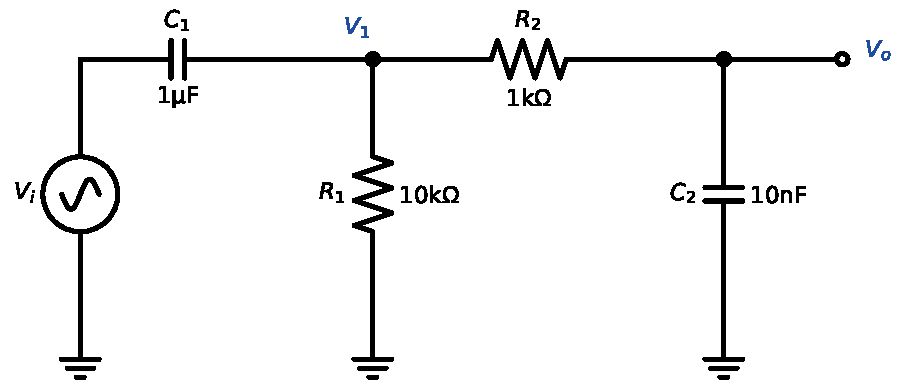
\includegraphics[width=0.95\linewidth,height=5.2cm,keepaspectratio]{p09_ac}\end{center}

\solstep{4}{Transfer function by a chain of dividers}Walk from the input to the output through the named nodes: $V_{i} \to V_{1} \to V_{o}$. The transfer function is the product of the node-to-node ratios (each one is a simple divider, tool T2, or a dependent source, tool T4):
\[
H(s) = \frac{V_o}{V_i} = \frac{V_{1}}{V_{i}}\cdot\frac{V_{o}}{V_{1}}
\]

Impedances seen \emph{looking right} from a node (everything from that node to ground, excluding what is on its left). Compute them from the far right toward the input:
\begin{align*}
Z_{1} &= R_{1} \parallel \left(R_{2} + \frac{1}{sC_{2}}\right) = \dfrac{909\,s + 9.09\times 10^{7}}{s + 9090}
\end{align*}

Now each link. {\small (Algebra tip: to simplify a fraction that contains fractions, multiply its top and bottom by every inner denominator; then divide top and bottom by the leading coefficient of the denominator so that it starts with a plain $s^n$.)}
\begin{align*}
\frac{V_{1}}{V_{i}} &= \frac{Z_{1}}{\frac{1}{sC_{1}} + Z_{1}} = \dfrac{s^{2} + 10^{5}\,s}{s^{2} + 1.01\times 10^{5}\,s + 10^{7}} \\
\frac{V_{o}}{V_{1}} &= \frac{\frac{1}{sC_{2}}}{R_{2} + \frac{1}{sC_{2}}} = \dfrac{10^{5}}{s + 10^{5}}
\end{align*}

Multiply the links and simplify (common factors cancel):\[
H(s) = \dfrac{10^{5}\,s}{s^{2} + 1.01\times 10^{5}\,s + 10^{7}}
\]

\solstep{5}{Standard (Bode-ready) form}Find the roots. Every root $s=-p$ of the denominator is a \emph{pole}, every root $s=-z$ of the numerator is a \emph{zero}; $|p|$ and $|z|$ are the corner frequencies (rad/s).
\begin{itemize}[leftmargin=*,itemsep=2pt]
\item Numerator: it has the factor $s$ $\Rightarrow$ 1 zero at $s=0$.
\item Denominator: $s^{2} + 1.01\times 10^{5}\,s + 10^{7}$; quadratic formula:\[
s = \frac{-1.01\times 10^{5} \pm \sqrt{(1.01\times 10^{5})^2 - 4(10^{7})}}{2} = \frac{-1.01\times 10^{5} \pm 1.01\times 10^{5}}{2} \Rightarrow s = -99,\ -1.01\times 10^{5}
\]

\end{itemize}

Factored form (leading coefficient in front):
\[
H(s) = 10^{5}\,\dfrac{s}{(s+99)(s+1.01\times 10^{5})}
\]

Bode-ready form: rewrite every $(s+p) = p\left(1+\frac{s}{p}\right)$ and $(s+z) = z\left(1+\frac{s}{z}\right)$, and collect all constants into $K$. Each $s$ in the numerator is paired with one of the \emph{lowest} poles as $\frac{s}{s+p}$ (that factor is $\approx 1$ above $p$). Then every factor except $K$ is $\approx 1$ inside the pass-band:
\[
H(s) = 0.99\,\dfrac{s}{s+2\pi\cdot 15.8}\,\dfrac{1}{1+\dfrac{s}{2\pi\cdot 16.1\mathrm{k}}},\qquad K = 0.99
\]

\begin{center}\renewcommand{\arraystretch}{1.35}
\begin{tabular}{cccc}
\toprule
type & $\omega_c$ (rad/s) & $f_c=\omega_c/2\pi$ & slope change \\
\midrule
pole & $99$ & 15.8 Hz & $-20$ dB/dec \\
pole & $1.01\times 10^{5}$ & 16.1 kHz & $-20$ dB/dec \\
\bottomrule
\end{tabular}\end{center}

\solstep{6}{Magnitude Bode plot}Below every corner $|H(s)|\approx 0.01\,s$, so the plot starts with a slope of $+20$\,dB/dec. Then, moving right, each pole bends the line down by 20\,dB/dec and each zero bends it up by 20\,dB/dec (tool T6):
\begin{center}\renewcommand{\arraystretch}{1.35}
\begin{tabular}{lcl}
\toprule
frequency range & slope & asymptote level \\
\midrule
$f<$ 15.8 Hz & $+20$ dB/dec & -0.0865 dB at end \\
15.8 Hz -- 16.1 kHz & $0$ dB/dec (flat) & -0.0865 dB at start, -0.0865 dB at end \\
$f>$ 16.1 kHz & $-20$ dB/dec & -0.0865 dB at start \\
\bottomrule
\end{tabular}\end{center}

The flat (pass-band) level is $20\log_{10}|K| = 20\log_{10}0.99 = -0.0865$\,dB.
\begin{center}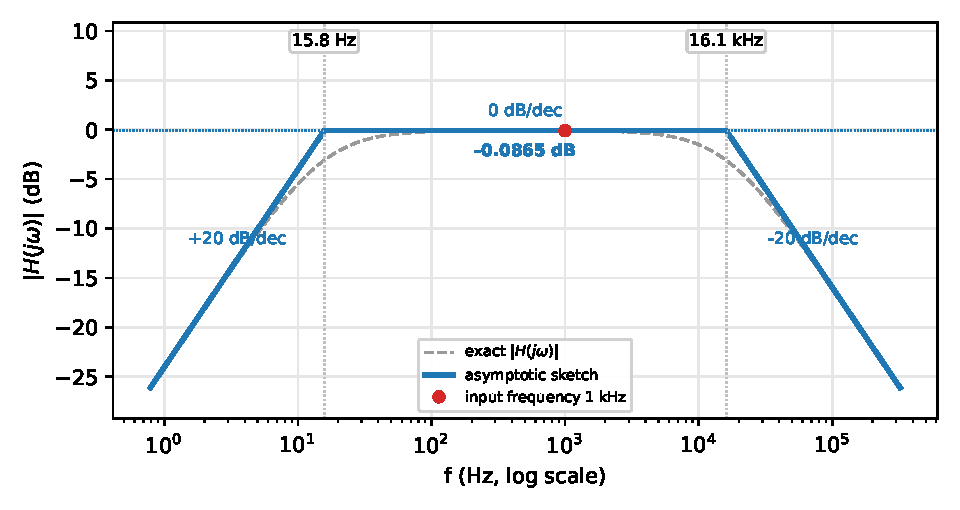
\includegraphics[width=0.78\linewidth,height=6.5cm,keepaspectratio]{p09_bode}\end{center}

{\small Blue: the straight-line sketch you are expected to draw. Dashed grey: the exact curve (about 3\,dB below the corner of an isolated pole). Red dot: the input frequency of Step 7.}
\solstep{7}{Steady-state output}The input is $V_i(t) = 1\sin\left(2\pi\cdot 1000\,t\right)$, so $\omega_{in} = 2\pi\cdot 1000 = 6280$\,rad/s. Put $s=j\omega_{in}$ in each factor (tool T5): magnitudes multiply, angles add.
{\small Rules: $\left|\frac{s}{s+p}\right| = \frac{\omega}{\sqrt{\omega^2+p^2}}$, $\angle = \frac{\pi}{2}-\tan^{-1}\frac{\omega}{p}$;\quad $\left|\frac{1}{1+s/p}\right| = \frac{1}{\sqrt{1+(\omega/p)^2}}$, $\angle = -\tan^{-1}\frac{\omega}{p}$;\quad $\left|1+\frac{s}{z}\right| = \sqrt{1+(\omega/z)^2}$, $\angle = \tan^{-1}\frac{\omega}{z}$;\quad a negative $K$ adds $-\pi$.}
\begin{center}\renewcommand{\arraystretch}{1.35}
\begin{tabular}{ccc}
\toprule
factor & magnitude & angle (rad) \\
\midrule
$0.99$ & $0.9901$ & $0$ \\
$\rule[-1.1em]{0pt}{2.8em}\dfrac{s}{s+2\pi\cdot 15.8}$ & $0.9999$ & $0.0158$ \\
$\rule[-1.7em]{0pt}{4em}\dfrac{1}{1+\dfrac{s}{2\pi\cdot 16.1\mathrm{k}}}$ & $0.9981$ & $-0.0621$ \\
\textbf{total} & $\mathbf{0.9881}$ (product) & $\mathbf{-0.0464}$ (sum) \\
\bottomrule
\end{tabular}\end{center}

\begin{align*}
|H(j\omega_{in})| &= 0.988, \qquad \angle H(j\omega_{in}) = -0.0464\ \mathrm{rad} \\
v_{o,ac}(t) &= 0.988\times 1\,\sin\left(2\pi\cdot 1000\,t - 0.0464\right) = 0.988\,\sin\left(2\pi\cdot 1000\,t - 0.0464\right)
\end{align*}

\[
\boxed{V_o(t) = 0.988\,\sin\left(2\pi\cdot 1000\,t - 0.0464\right)\ \mathrm{V}}
\]

\begin{ansbox}
$H(s) = 0.99\,\dfrac{s}{s+2\pi\cdot 15.8}\,\dfrac{1}{1+\dfrac{s}{2\pi\cdot 16.1\mathrm{k}}}$\quad (corners: 15.8 Hz, 16.1 kHz)\\[4pt]
$V_o(t) = 0.988\,\sin\left(2\pi\cdot 1000\,t - 0.0464\right)\ \mathrm{V}$
\end{ansbox}

\newpage
\subsection*{Solution 1A.10 \hfill Medium}
\begin{center}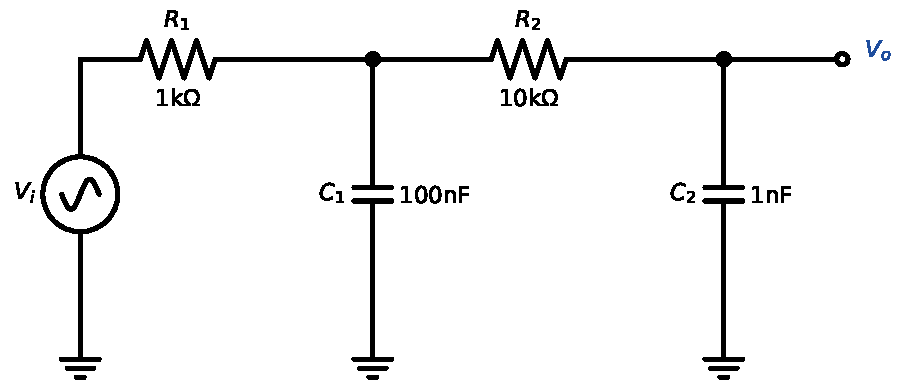
\includegraphics[width=0.8\linewidth,height=4.5cm,keepaspectratio]{p10_circuit}\end{center}
\solstep{1}{Identify the sources}Independent sources: the AC input $V_i(t)$. There is no DC source, so $V_{o,dc}=0$ and $V_o(t)=v_{o,ac}(t)$: Step 2 is skipped.
\solstep{2}{DC circuit}No DC sources: $V_{o,dc}=0$.
\solstep{3}{AC circuit}Replace every capacitor by $\frac{1}{sC}$ and every inductor by $sL$.
AC equivalent circuit (nodes named for the next step):
\begin{center}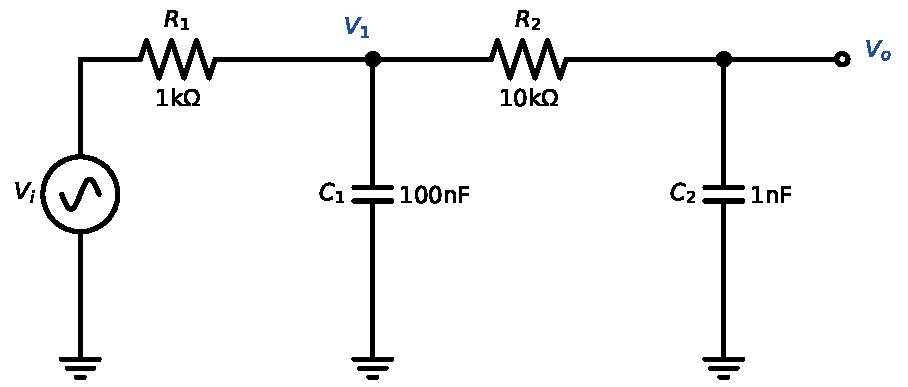
\includegraphics[width=0.95\linewidth,height=5.2cm,keepaspectratio]{p10_ac}\end{center}

\solstep{4}{Transfer function by a chain of dividers}Walk from the input to the output through the named nodes: $V_{i} \to V_{1} \to V_{o}$. The transfer function is the product of the node-to-node ratios (each one is a simple divider, tool T2, or a dependent source, tool T4):
\[
H(s) = \frac{V_o}{V_i} = \frac{V_{1}}{V_{i}}\cdot\frac{V_{o}}{V_{1}}
\]

Impedances seen \emph{looking right} from a node (everything from that node to ground, excluding what is on its left). Compute them from the far right toward the input:
\begin{align*}
Z_{1} &= \frac{1}{sC_{1}} \parallel \left(R_{2} + \frac{1}{sC_{2}}\right) = \dfrac{10^{7}\,s + 10^{12}}{s^{2} + 1.01\times 10^{5}\,s}
\end{align*}

Now each link. {\small (Algebra tip: to simplify a fraction that contains fractions, multiply its top and bottom by every inner denominator; then divide top and bottom by the leading coefficient of the denominator so that it starts with a plain $s^n$.)}
\begin{align*}
\frac{V_{1}}{V_{i}} &= \frac{Z_{1}}{R_{1} + Z_{1}} = \dfrac{10000\,s + 10^{9}}{s^{2} + 1.11\times 10^{5}\,s + 10^{9}} \\
\frac{V_{o}}{V_{1}} &= \frac{\frac{1}{sC_{2}}}{R_{2} + \frac{1}{sC_{2}}} = \dfrac{10^{5}}{s + 10^{5}}
\end{align*}

Multiply the links and simplify (common factors cancel):\[
H(s) = \dfrac{10^{9}}{s^{2} + 1.11\times 10^{5}\,s + 10^{9}}
\]

\solstep{5}{Standard (Bode-ready) form}Find the roots. Every root $s=-p$ of the denominator is a \emph{pole}, every root $s=-z$ of the numerator is a \emph{zero}; $|p|$ and $|z|$ are the corner frequencies (rad/s).
\begin{itemize}[leftmargin=*,itemsep=2pt]
\item Denominator: $s^{2} + 1.11\times 10^{5}\,s + 10^{9}$; quadratic formula:\[
s = \frac{-1.11\times 10^{5} \pm \sqrt{(1.11\times 10^{5})^2 - 4(10^{9})}}{2} = \frac{-1.11\times 10^{5} \pm 91200}{2} \Rightarrow s = -9890,\ -1.01\times 10^{5}
\]

\end{itemize}

Factored form (leading coefficient in front):
\[
H(s) = 10^{9}\,\dfrac{1}{(s+9890)(s+1.01\times 10^{5})}
\]

Bode-ready form: rewrite every $(s+p) = p\left(1+\frac{s}{p}\right)$ and $(s+z) = z\left(1+\frac{s}{z}\right)$, and collect all constants into $K$. Then every factor except $K$ is $\approx 1$ inside the pass-band:
\[
H(s) = 1\,\dfrac{1}{1+\dfrac{s}{2\pi\cdot 1.57\mathrm{k}}}\,\dfrac{1}{1+\dfrac{s}{2\pi\cdot 16.1\mathrm{k}}},\qquad K = 1
\]

\begin{center}\renewcommand{\arraystretch}{1.35}
\begin{tabular}{cccc}
\toprule
type & $\omega_c$ (rad/s) & $f_c=\omega_c/2\pi$ & slope change \\
\midrule
pole & $9890$ & 1.57 kHz & $-20$ dB/dec \\
pole & $1.01\times 10^{5}$ & 16.1 kHz & $-20$ dB/dec \\
\bottomrule
\end{tabular}\end{center}

\solstep{6}{Magnitude Bode plot}Below every corner, all factors are $\approx$ constant: $|H| \approx 1$ $= -0.000000000000000964$\,dB (flat, 0 dB/dec). Then, moving right, each pole bends the line down by 20\,dB/dec and each zero bends it up by 20\,dB/dec (tool T6):
\begin{center}\renewcommand{\arraystretch}{1.35}
\begin{tabular}{lcl}
\toprule
frequency range & slope & asymptote level \\
\midrule
$f<$ 1.57 kHz & $0$ dB/dec (flat) & 0 dB at end \\
1.57 kHz -- 16.1 kHz & $-20$ dB/dec & 0 dB at start, -20.2 dB at end \\
$f>$ 16.1 kHz & $-40$ dB/dec & -20.2 dB at start \\
\bottomrule
\end{tabular}\end{center}

The flat (pass-band) level is $20\log_{10}|K| = 20\log_{10}1 = -0.000000000000000964$\,dB.
\begin{center}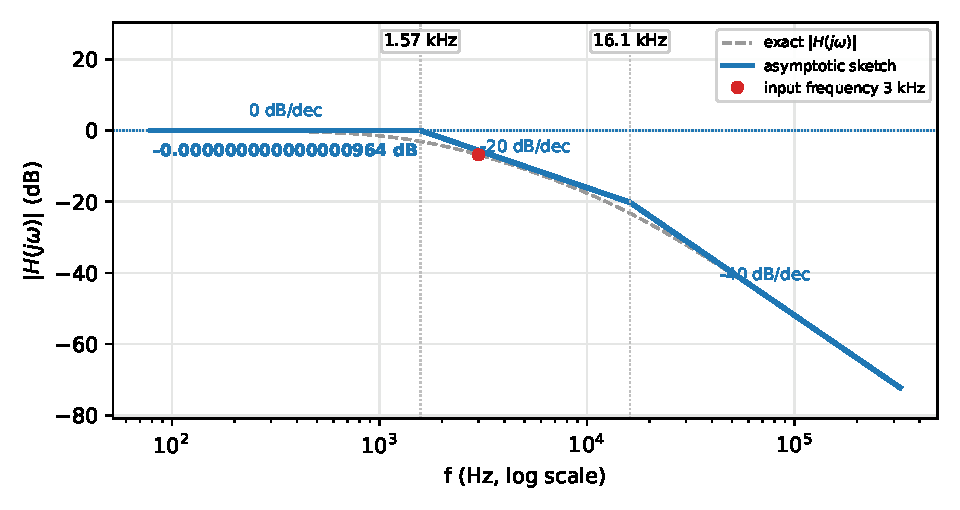
\includegraphics[width=0.78\linewidth,height=6.5cm,keepaspectratio]{p10_bode}\end{center}

{\small Blue: the straight-line sketch you are expected to draw. Dashed grey: the exact curve (about 3\,dB below the corner of an isolated pole). Red dot: the input frequency of Step 7.}
\solstep{7}{Steady-state output}The input is $V_i(t) = 1\sin\left(2\pi\cdot 3000\,t\right)$, so $\omega_{in} = 2\pi\cdot 3000 = 18800$\,rad/s. Put $s=j\omega_{in}$ in each factor (tool T5): magnitudes multiply, angles add.
{\small Rules: $\left|\frac{s}{s+p}\right| = \frac{\omega}{\sqrt{\omega^2+p^2}}$, $\angle = \frac{\pi}{2}-\tan^{-1}\frac{\omega}{p}$;\quad $\left|\frac{1}{1+s/p}\right| = \frac{1}{\sqrt{1+(\omega/p)^2}}$, $\angle = -\tan^{-1}\frac{\omega}{p}$;\quad $\left|1+\frac{s}{z}\right| = \sqrt{1+(\omega/z)^2}$, $\angle = \tan^{-1}\frac{\omega}{z}$;\quad a negative $K$ adds $-\pi$.}
\begin{center}\renewcommand{\arraystretch}{1.35}
\begin{tabular}{ccc}
\toprule
factor & magnitude & angle (rad) \\
\midrule
$1$ & $1$ & $0$ \\
$\rule[-1.7em]{0pt}{4em}\dfrac{1}{1+\dfrac{s}{2\pi\cdot 1.57\mathrm{k}}}$ & $0.4646$ & $-1.09$ \\
$\rule[-1.7em]{0pt}{4em}\dfrac{1}{1+\dfrac{s}{2\pi\cdot 16.1\mathrm{k}}}$ & $0.9831$ & $-0.184$ \\
\textbf{total} & $\mathbf{0.4568}$ (product) & $\mathbf{-1.27}$ (sum) \\
\bottomrule
\end{tabular}\end{center}

\begin{align*}
|H(j\omega_{in})| &= 0.457, \qquad \angle H(j\omega_{in}) = -1.27\ \mathrm{rad} \\
v_{o,ac}(t) &= 0.457\times 1\,\sin\left(2\pi\cdot 3000\,t - 1.27\right) = 0.457\,\sin\left(2\pi\cdot 3000\,t - 1.27\right)
\end{align*}

\[
\boxed{V_o(t) = 0.457\,\sin\left(2\pi\cdot 3000\,t - 1.27\right)\ \mathrm{V}}
\]

\begin{ansbox}
$H(s) = 1\,\dfrac{1}{1+\dfrac{s}{2\pi\cdot 1.57\mathrm{k}}}\,\dfrac{1}{1+\dfrac{s}{2\pi\cdot 16.1\mathrm{k}}}$\quad (corners: 1.57 kHz, 16.1 kHz)\\[4pt]
$V_o(t) = 0.457\,\sin\left(2\pi\cdot 3000\,t - 1.27\right)\ \mathrm{V}$
\end{ansbox}

\newpage
\subsection*{Solution 1A.11 \hfill Medium}
\begin{center}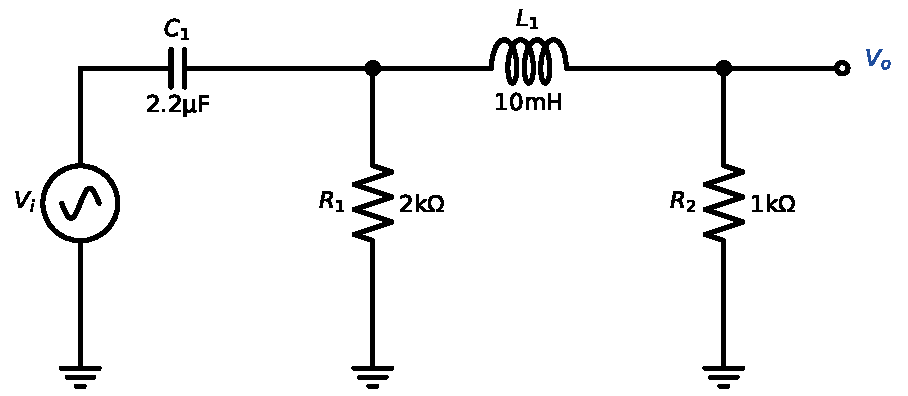
\includegraphics[width=0.8\linewidth,height=4.5cm,keepaspectratio]{p11_circuit}\end{center}
\solstep{1}{Identify the sources}Independent sources: the AC input $V_i(t)$. There is no DC source, so $V_{o,dc}=0$ and $V_o(t)=v_{o,ac}(t)$: Step 2 is skipped.
\solstep{2}{DC circuit}No DC sources: $V_{o,dc}=0$.
\solstep{3}{AC circuit}Replace every capacitor by $\frac{1}{sC}$ and every inductor by $sL$.
AC equivalent circuit (nodes named for the next step):
\begin{center}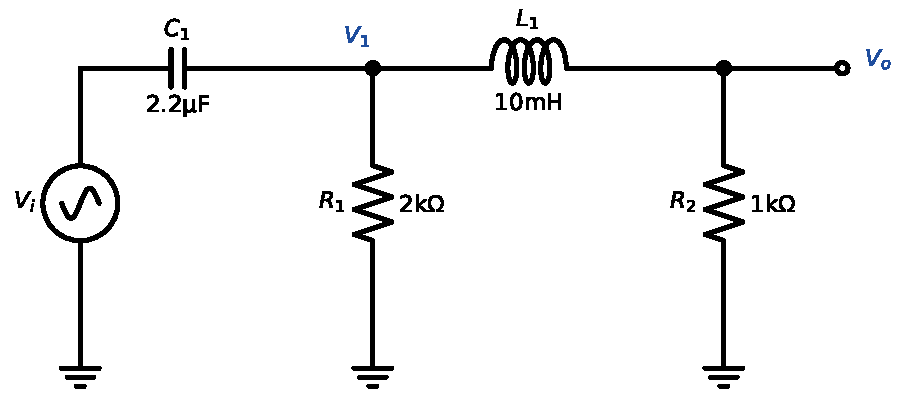
\includegraphics[width=0.95\linewidth,height=5.2cm,keepaspectratio]{p11_ac}\end{center}

\solstep{4}{Transfer function by a chain of dividers}Walk from the input to the output through the named nodes: $V_{i} \to V_{1} \to V_{o}$. The transfer function is the product of the node-to-node ratios (each one is a simple divider, tool T2, or a dependent source, tool T4):
\[
H(s) = \frac{V_o}{V_i} = \frac{V_{1}}{V_{i}}\cdot\frac{V_{o}}{V_{1}}
\]

Impedances seen \emph{looking right} from a node (everything from that node to ground, excluding what is on its left). Compute them from the far right toward the input:
\begin{align*}
Z_{1} &= R_{1} \parallel \left(sL_{1} + R_{2}\right) = \dfrac{2000\,s + 2\times 10^{8}}{s + 3\times 10^{5}}
\end{align*}

Now each link. {\small (Algebra tip: to simplify a fraction that contains fractions, multiply its top and bottom by every inner denominator; then divide top and bottom by the leading coefficient of the denominator so that it starts with a plain $s^n$.)}
\begin{align*}
\frac{V_{1}}{V_{i}} &= \frac{Z_{1}}{\frac{1}{sC_{1}} + Z_{1}} = \dfrac{s^{2} + 10^{5}\,s}{s^{2} + 10^{5}\,s + 6.82\times 10^{7}} \\
\frac{V_{o}}{V_{1}} &= \frac{R_{2}}{sL_{1} + R_{2}} = \dfrac{10^{5}}{s + 10^{5}}
\end{align*}

Multiply the links and simplify (common factors cancel):\[
H(s) = \dfrac{10^{5}\,s}{s^{2} + 10^{5}\,s + 6.82\times 10^{7}}
\]

\solstep{5}{Standard (Bode-ready) form}Find the roots. Every root $s=-p$ of the denominator is a \emph{pole}, every root $s=-z$ of the numerator is a \emph{zero}; $|p|$ and $|z|$ are the corner frequencies (rad/s).
\begin{itemize}[leftmargin=*,itemsep=2pt]
\item Numerator: it has the factor $s$ $\Rightarrow$ 1 zero at $s=0$.
\item Denominator: $s^{2} + 10^{5}\,s + 6.82\times 10^{7}$; quadratic formula:\[
s = \frac{-10^{5} \pm \sqrt{(10^{5})^2 - 4(6.82\times 10^{7})}}{2} = \frac{-10^{5} \pm 98900}{2} \Rightarrow s = -685,\ -99500
\]

\end{itemize}

Factored form (leading coefficient in front):
\[
H(s) = 10^{5}\,\dfrac{s}{(s+685)(s+99500)}
\]

Bode-ready form: rewrite every $(s+p) = p\left(1+\frac{s}{p}\right)$ and $(s+z) = z\left(1+\frac{s}{z}\right)$, and collect all constants into $K$. Each $s$ in the numerator is paired with one of the \emph{lowest} poles as $\frac{s}{s+p}$ (that factor is $\approx 1$ above $p$). Then every factor except $K$ is $\approx 1$ inside the pass-band:
\[
H(s) = 1\,\dfrac{s}{s+2\pi\cdot 109}\,\dfrac{1}{1+\dfrac{s}{2\pi\cdot 15.8\mathrm{k}}},\qquad K = 1
\]

\begin{center}\renewcommand{\arraystretch}{1.35}
\begin{tabular}{cccc}
\toprule
type & $\omega_c$ (rad/s) & $f_c=\omega_c/2\pi$ & slope change \\
\midrule
pole & $685$ & 109 Hz & $-20$ dB/dec \\
pole & $99500$ & 15.8 kHz & $-20$ dB/dec \\
\bottomrule
\end{tabular}\end{center}

\solstep{6}{Magnitude Bode plot}Below every corner $|H(s)|\approx 0.00147\,s$, so the plot starts with a slope of $+20$\,dB/dec. Then, moving right, each pole bends the line down by 20\,dB/dec and each zero bends it up by 20\,dB/dec (tool T6):
\begin{center}\renewcommand{\arraystretch}{1.35}
\begin{tabular}{lcl}
\toprule
frequency range & slope & asymptote level \\
\midrule
$f<$ 109 Hz & $+20$ dB/dec & 0.0398 dB at end \\
109 Hz -- 15.8 kHz & $0$ dB/dec (flat) & 0.0398 dB at start, 0.0398 dB at end \\
$f>$ 15.8 kHz & $-20$ dB/dec & 0.0398 dB at start \\
\bottomrule
\end{tabular}\end{center}

The flat (pass-band) level is $20\log_{10}|K| = 20\log_{10}1 = 0.0398$\,dB.
\begin{center}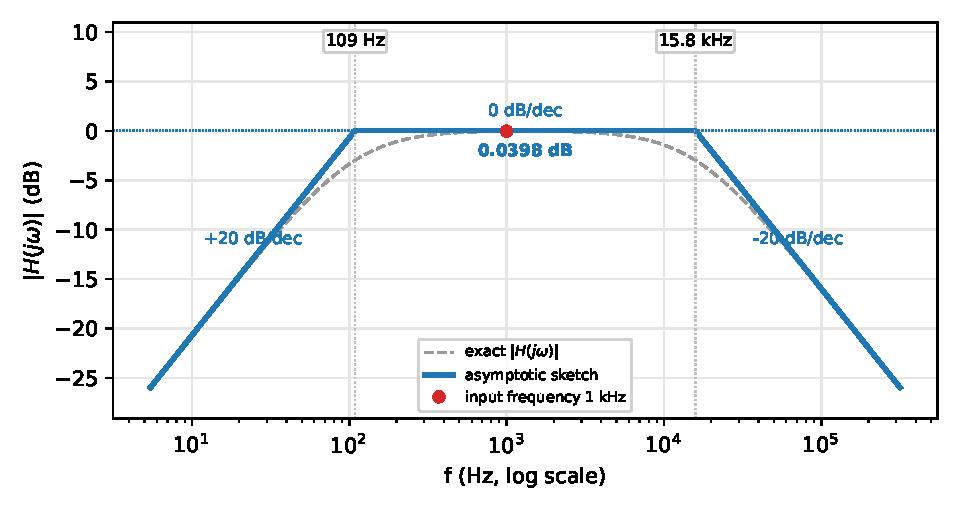
\includegraphics[width=0.78\linewidth,height=6.5cm,keepaspectratio]{p11_bode}\end{center}

{\small Blue: the straight-line sketch you are expected to draw. Dashed grey: the exact curve (about 3\,dB below the corner of an isolated pole). Red dot: the input frequency of Step 7.}
\solstep{7}{Steady-state output}The input is $V_i(t) = 2\sin\left(2\pi\cdot 1000\,t\right)$, so $\omega_{in} = 2\pi\cdot 1000 = 6280$\,rad/s. Put $s=j\omega_{in}$ in each factor (tool T5): magnitudes multiply, angles add.
{\small Rules: $\left|\frac{s}{s+p}\right| = \frac{\omega}{\sqrt{\omega^2+p^2}}$, $\angle = \frac{\pi}{2}-\tan^{-1}\frac{\omega}{p}$;\quad $\left|\frac{1}{1+s/p}\right| = \frac{1}{\sqrt{1+(\omega/p)^2}}$, $\angle = -\tan^{-1}\frac{\omega}{p}$;\quad $\left|1+\frac{s}{z}\right| = \sqrt{1+(\omega/z)^2}$, $\angle = \tan^{-1}\frac{\omega}{z}$;\quad a negative $K$ adds $-\pi$.}
\begin{center}\renewcommand{\arraystretch}{1.35}
\begin{tabular}{ccc}
\toprule
factor & magnitude & angle (rad) \\
\midrule
$1$ & $1.005$ & $0$ \\
$\rule[-1.1em]{0pt}{2.8em}\dfrac{s}{s+2\pi\cdot 109}$ & $0.9941$ & $0.109$ \\
$\rule[-1.7em]{0pt}{4em}\dfrac{1}{1+\dfrac{s}{2\pi\cdot 15.8\mathrm{k}}}$ & $0.998$ & $-0.063$ \\
\textbf{total} & $\mathbf{0.9967}$ (product) & $\mathbf{0.0455}$ (sum) \\
\bottomrule
\end{tabular}\end{center}

\begin{align*}
|H(j\omega_{in})| &= 0.997, \qquad \angle H(j\omega_{in}) = 0.0455\ \mathrm{rad} \\
v_{o,ac}(t) &= 0.997\times 2\,\sin\left(2\pi\cdot 1000\,t + 0.0455\right) = 1.99\,\sin\left(2\pi\cdot 1000\,t + 0.0455\right)
\end{align*}

\[
\boxed{V_o(t) = 1.99\,\sin\left(2\pi\cdot 1000\,t + 0.0455\right)\ \mathrm{V}}
\]

\begin{ansbox}
$H(s) = 1\,\dfrac{s}{s+2\pi\cdot 109}\,\dfrac{1}{1+\dfrac{s}{2\pi\cdot 15.8\mathrm{k}}}$\quad (corners: 109 Hz, 15.8 kHz)\\[4pt]
$V_o(t) = 1.99\,\sin\left(2\pi\cdot 1000\,t + 0.0455\right)\ \mathrm{V}$
\end{ansbox}

\newpage
\subsection*{Solution 1A.12 \hfill Medium}
\begin{center}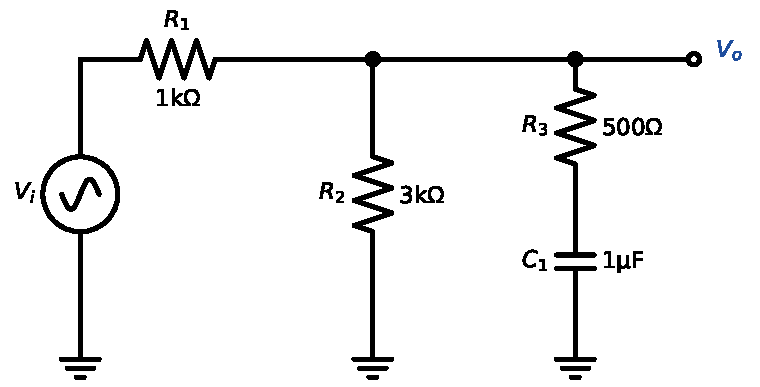
\includegraphics[width=0.8\linewidth,height=4.5cm,keepaspectratio]{p12_circuit}\end{center}
\solstep{1}{Identify the sources}Independent sources: the AC input $V_i(t)$. There is no DC source, so $V_{o,dc}=0$ and $V_o(t)=v_{o,ac}(t)$: Step 2 is skipped.
\solstep{2}{DC circuit}No DC sources: $V_{o,dc}=0$.
\solstep{3}{AC circuit}Replace every capacitor by $\frac{1}{sC}$ and every inductor by $sL$.
AC equivalent circuit (nodes named for the next step):
\begin{center}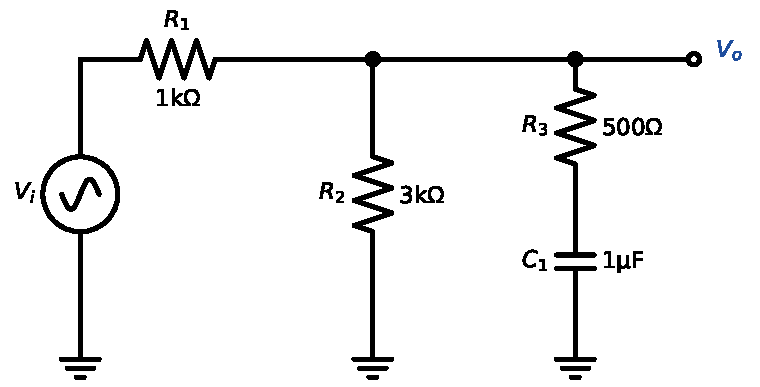
\includegraphics[width=0.95\linewidth,height=5.2cm,keepaspectratio]{p12_ac}\end{center}

\solstep{4}{Transfer function by a chain of dividers}Walk from the input to the output through the named nodes: $V_{i} \to V_{o}$. There is a single link, so $H(s)$ is just one voltage divider (tool T2).
Impedances seen \emph{looking right} from a node (everything from that node to ground, excluding what is on its left). Compute them from the far right toward the input:
\begin{align*}
Z_{o} &= R_{2} \parallel \left(R_{3} + \frac{1}{sC_{1}}\right) = \dfrac{429\,s + 8.57\times 10^{5}}{s + 286}
\end{align*}

Now each link. {\small (Algebra tip: to simplify a fraction that contains fractions, multiply its top and bottom by every inner denominator; then divide top and bottom by the leading coefficient of the denominator so that it starts with a plain $s^n$.)}
\begin{align*}
\frac{V_{o}}{V_{i}} &= \frac{Z_{o}}{R_{1} + Z_{o}} = \dfrac{0.3\,s + 600}{s + 800}
\end{align*}

So:\[
H(s) = \dfrac{0.3\,s + 600}{s + 800}
\]

\solstep{5}{Standard (Bode-ready) form}Find the roots. Every root $s=-p$ of the denominator is a \emph{pole}, every root $s=-z$ of the numerator is a \emph{zero}; $|p|$ and $|z|$ are the corner frequencies (rad/s).
\begin{itemize}[leftmargin=*,itemsep=2pt]
\item Numerator: $0.3\,s + 600$; divide by the leading coefficient $0.3$ (this does not move the roots): $s + 2000$; $s + 2000 = 0 \Rightarrow s = -2000$.
\item Denominator: $s + 800$; $s + 800 = 0 \Rightarrow s = -800$.
\end{itemize}

Factored form (leading coefficient in front):
\[
H(s) = 0.3\,\dfrac{(s+2000)}{(s+800)}
\]

Bode-ready form: rewrite every $(s+p) = p\left(1+\frac{s}{p}\right)$ and $(s+z) = z\left(1+\frac{s}{z}\right)$, and collect all constants into $K$. Then every factor except $K$ is $\approx 1$ inside the pass-band:
\[
H(s) = 0.75\,\dfrac{1}{1+\dfrac{s}{2\pi\cdot 127}}\,\left(1+\dfrac{s}{2\pi\cdot 318}\right),\qquad K = 0.75
\]

\begin{center}\renewcommand{\arraystretch}{1.35}
\begin{tabular}{cccc}
\toprule
type & $\omega_c$ (rad/s) & $f_c=\omega_c/2\pi$ & slope change \\
\midrule
pole & $800$ & 127 Hz & $-20$ dB/dec \\
zero & $2000$ & 318 Hz & $+20$ dB/dec \\
\bottomrule
\end{tabular}\end{center}

\solstep{6}{Magnitude Bode plot}Below every corner, all factors are $\approx$ constant: $|H| \approx 0.75$ $= -2.5$\,dB (flat, 0 dB/dec). Then, moving right, each pole bends the line down by 20\,dB/dec and each zero bends it up by 20\,dB/dec (tool T6):
\begin{center}\renewcommand{\arraystretch}{1.35}
\begin{tabular}{lcl}
\toprule
frequency range & slope & asymptote level \\
\midrule
$f<$ 127 Hz & $0$ dB/dec (flat) & -2.5 dB at end \\
127 Hz -- 318 Hz & $-20$ dB/dec & -2.5 dB at start, -10.5 dB at end \\
$f>$ 318 Hz & $0$ dB/dec (flat) & -10.5 dB at start \\
\bottomrule
\end{tabular}\end{center}

\begin{center}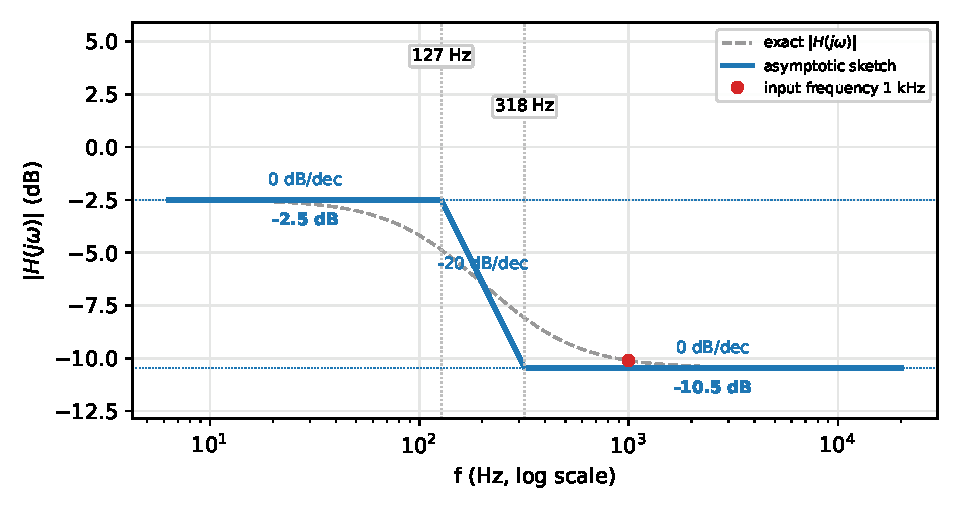
\includegraphics[width=0.78\linewidth,height=6.5cm,keepaspectratio]{p12_bode}\end{center}

{\small Blue: the straight-line sketch you are expected to draw. Dashed grey: the exact curve (about 3\,dB below the corner of an isolated pole). Red dot: the input frequency of Step 7.}
\solstep{7}{Steady-state output}The input is $V_i(t) = 1\sin\left(2\pi\cdot 1000\,t\right)$, so $\omega_{in} = 2\pi\cdot 1000 = 6280$\,rad/s. Put $s=j\omega_{in}$ in each factor (tool T5): magnitudes multiply, angles add.
{\small Rules: $\left|\frac{s}{s+p}\right| = \frac{\omega}{\sqrt{\omega^2+p^2}}$, $\angle = \frac{\pi}{2}-\tan^{-1}\frac{\omega}{p}$;\quad $\left|\frac{1}{1+s/p}\right| = \frac{1}{\sqrt{1+(\omega/p)^2}}$, $\angle = -\tan^{-1}\frac{\omega}{p}$;\quad $\left|1+\frac{s}{z}\right| = \sqrt{1+(\omega/z)^2}$, $\angle = \tan^{-1}\frac{\omega}{z}$;\quad a negative $K$ adds $-\pi$.}
\begin{center}\renewcommand{\arraystretch}{1.35}
\begin{tabular}{ccc}
\toprule
factor & magnitude & angle (rad) \\
\midrule
$0.75$ & $0.75$ & $0$ \\
$\rule[-1.7em]{0pt}{4em}\dfrac{1}{1+\dfrac{s}{2\pi\cdot 127}}$ & $0.1263$ & $-1.44$ \\
$\rule[-1.1em]{0pt}{2.8em}\left(1+\dfrac{s}{2\pi\cdot 318}\right)$ & $3.297$ & $1.26$ \\
\textbf{total} & $\mathbf{0.3123}$ (product) & $\mathbf{-0.182}$ (sum) \\
\bottomrule
\end{tabular}\end{center}

\begin{align*}
|H(j\omega_{in})| &= 0.312, \qquad \angle H(j\omega_{in}) = -0.182\ \mathrm{rad} \\
v_{o,ac}(t) &= 0.312\times 1\,\sin\left(2\pi\cdot 1000\,t - 0.182\right) = 0.312\,\sin\left(2\pi\cdot 1000\,t - 0.182\right)
\end{align*}

\[
\boxed{V_o(t) = 0.312\,\sin\left(2\pi\cdot 1000\,t - 0.182\right)\ \mathrm{V}}
\]

\begin{ansbox}
$H(s) = 0.75\,\dfrac{1}{1+\dfrac{s}{2\pi\cdot 127}}\,\left(1+\dfrac{s}{2\pi\cdot 318}\right)$\quad (corners: 127 Hz, 318 Hz)\\[4pt]
$V_o(t) = 0.312\,\sin\left(2\pi\cdot 1000\,t - 0.182\right)\ \mathrm{V}$
\end{ansbox}

\newpage
\subsection*{Solution 1A.13 \hfill Hard}
\begin{center}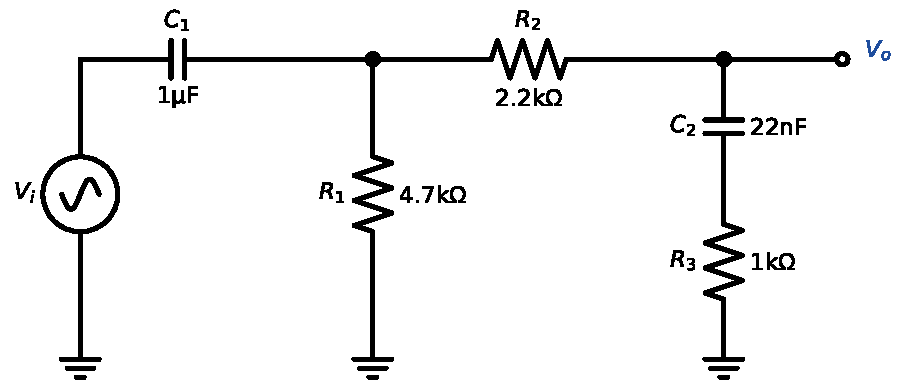
\includegraphics[width=0.8\linewidth,height=4.5cm,keepaspectratio]{p13_circuit}\end{center}
\solstep{1}{Identify the sources}Independent sources: the AC input $V_i(t)$. There is no DC source, so $V_{o,dc}=0$ and $V_o(t)=v_{o,ac}(t)$: Step 2 is skipped.
\solstep{2}{DC circuit}No DC sources: $V_{o,dc}=0$.
\solstep{3}{AC circuit}Replace every capacitor by $\frac{1}{sC}$ and every inductor by $sL$.
AC equivalent circuit (nodes named for the next step):
\begin{center}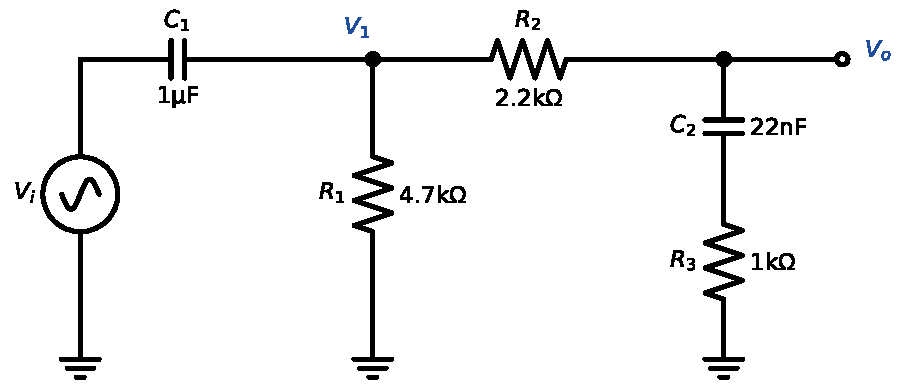
\includegraphics[width=0.95\linewidth,height=5.2cm,keepaspectratio]{p13_ac}\end{center}

\solstep{4}{Transfer function by a chain of dividers}Walk from the input to the output through the named nodes: $V_{i} \to V_{1} \to V_{o}$. The transfer function is the product of the node-to-node ratios (each one is a simple divider, tool T2, or a dependent source, tool T4):
\[
H(s) = \frac{V_o}{V_i} = \frac{V_{1}}{V_{i}}\cdot\frac{V_{o}}{V_{1}}
\]

Impedances seen \emph{looking right} from a node (everything from that node to ground, excluding what is on its left). Compute them from the far right toward the input:
\begin{align*}
Z_{o} &= \frac{1}{sC_{2}} + R_{3} = \dfrac{1000\,s + 4.55\times 10^{7}}{s} \\
Z_{1} &= R_{1} \parallel \left(R_{2} + Z_{o}\right) = \dfrac{1900\,s + 2.7\times 10^{7}}{s + 5750}
\end{align*}

Now each link. {\small (Algebra tip: to simplify a fraction that contains fractions, multiply its top and bottom by every inner denominator; then divide top and bottom by the leading coefficient of the denominator so that it starts with a plain $s^n$.)}
\begin{align*}
\frac{V_{1}}{V_{i}} &= \frac{Z_{1}}{\frac{1}{sC_{1}} + Z_{1}} = \dfrac{s^{2} + 14200\,s}{s^{2} + 14700\,s + 3.02\times 10^{6}} \\
\frac{V_{o}}{V_{1}} &= \frac{Z_{o}}{R_{2} + Z_{o}} = \dfrac{0.312\,s + 14200}{s + 14200}
\end{align*}

Multiply the links and simplify (common factors cancel):\[
H(s) = \dfrac{0.312\,s^{2} + 14200\,s}{s^{2} + 14700\,s + 3.02\times 10^{6}}
\]

\solstep{5}{Standard (Bode-ready) form}Find the roots. Every root $s=-p$ of the denominator is a \emph{pole}, every root $s=-z$ of the numerator is a \emph{zero}; $|p|$ and $|z|$ are the corner frequencies (rad/s).
\begin{itemize}[leftmargin=*,itemsep=2pt]
\item Numerator: it has the factor $s$ $\Rightarrow$ 1 zero at $s=0$.
\item Numerator (after taking out the $s$ factor): $0.312\,s + 14200$; divide by the leading coefficient $0.312$ (this does not move the roots): $s + 45500$; $s + 45500 = 0 \Rightarrow s = -45500$.
\item Denominator: $s^{2} + 14700\,s + 3.02\times 10^{6}$; quadratic formula:\[
s = \frac{-14700 \pm \sqrt{(14700)^2 - 4(3.02\times 10^{6})}}{2} = \frac{-14700 \pm 14300}{2} \Rightarrow s = -208,\ -14500
\]

\end{itemize}

Factored form (leading coefficient in front):
\[
H(s) = 0.312\,\dfrac{s(s+45500)}{(s+208)(s+14500)}
\]

Bode-ready form: rewrite every $(s+p) = p\left(1+\frac{s}{p}\right)$ and $(s+z) = z\left(1+\frac{s}{z}\right)$, and collect all constants into $K$. Each $s$ in the numerator is paired with one of the \emph{lowest} poles as $\frac{s}{s+p}$ (that factor is $\approx 1$ above $p$). Then every factor except $K$ is $\approx 1$ inside the pass-band:
\[
H(s) = 0.978\,\dfrac{s}{s+2\pi\cdot 33.1}\,\dfrac{1}{1+\dfrac{s}{2\pi\cdot 2.31\mathrm{k}}}\,\left(1+\dfrac{s}{2\pi\cdot 7.23\mathrm{k}}\right),\qquad K = 0.978
\]

\begin{center}\renewcommand{\arraystretch}{1.35}
\begin{tabular}{cccc}
\toprule
type & $\omega_c$ (rad/s) & $f_c=\omega_c/2\pi$ & slope change \\
\midrule
pole & $208$ & 33.1 Hz & $-20$ dB/dec \\
pole & $14500$ & 2.31 kHz & $-20$ dB/dec \\
zero & $45500$ & 7.23 kHz & $+20$ dB/dec \\
\bottomrule
\end{tabular}\end{center}

\solstep{6}{Magnitude Bode plot}Below every corner $|H(s)|\approx 0.0047\,s$, so the plot starts with a slope of $+20$\,dB/dec. Then, moving right, each pole bends the line down by 20\,dB/dec and each zero bends it up by 20\,dB/dec (tool T6):
\begin{center}\renewcommand{\arraystretch}{1.35}
\begin{tabular}{lcl}
\toprule
frequency range & slope & asymptote level \\
\midrule
$f<$ 33.1 Hz & $+20$ dB/dec & -0.192 dB at end \\
33.1 Hz -- 2.31 kHz & $0$ dB/dec (flat) & -0.192 dB at start, -0.192 dB at end \\
2.31 kHz -- 7.23 kHz & $-20$ dB/dec & -0.192 dB at start, -10.1 dB at end \\
$f>$ 7.23 kHz & $0$ dB/dec (flat) & -10.1 dB at start \\
\bottomrule
\end{tabular}\end{center}

\begin{center}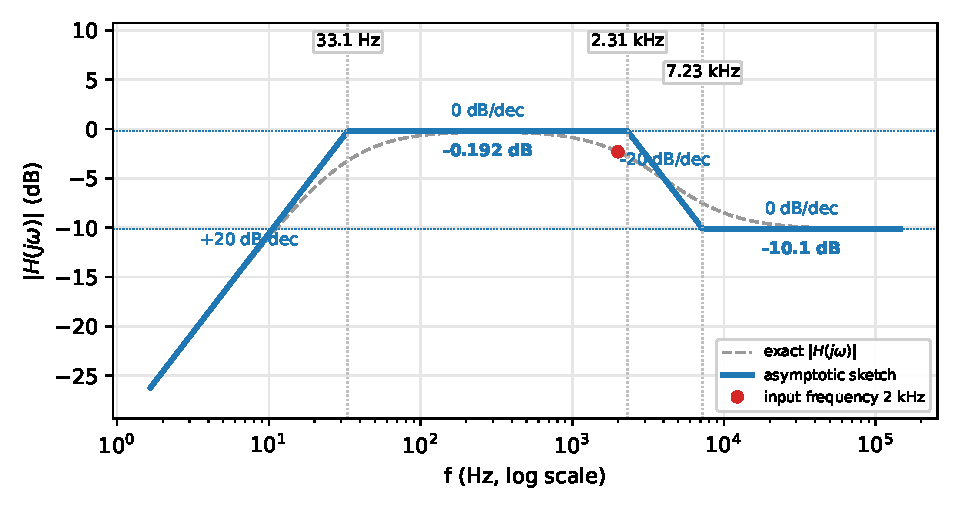
\includegraphics[width=0.78\linewidth,height=6.5cm,keepaspectratio]{p13_bode}\end{center}

{\small Blue: the straight-line sketch you are expected to draw. Dashed grey: the exact curve (about 3\,dB below the corner of an isolated pole). Red dot: the input frequency of Step 7.}
\solstep{7}{Steady-state output}The input is $V_i(t) = 1\cos\left(2\pi\cdot 2000\,t+\frac{\pi}{4}\right)$, so $\omega_{in} = 2\pi\cdot 2000 = 12600$\,rad/s. Put $s=j\omega_{in}$ in each factor (tool T5): magnitudes multiply, angles add.
{\small Rules: $\left|\frac{s}{s+p}\right| = \frac{\omega}{\sqrt{\omega^2+p^2}}$, $\angle = \frac{\pi}{2}-\tan^{-1}\frac{\omega}{p}$;\quad $\left|\frac{1}{1+s/p}\right| = \frac{1}{\sqrt{1+(\omega/p)^2}}$, $\angle = -\tan^{-1}\frac{\omega}{p}$;\quad $\left|1+\frac{s}{z}\right| = \sqrt{1+(\omega/z)^2}$, $\angle = \tan^{-1}\frac{\omega}{z}$;\quad a negative $K$ adds $-\pi$.}
\begin{center}\renewcommand{\arraystretch}{1.35}
\begin{tabular}{ccc}
\toprule
factor & magnitude & angle (rad) \\
\midrule
$0.978$ & $0.9782$ & $0$ \\
$\rule[-1.1em]{0pt}{2.8em}\dfrac{s}{s+2\pi\cdot 33.1}$ & $0.9999$ & $0.0166$ \\
$\rule[-1.7em]{0pt}{4em}\dfrac{1}{1+\dfrac{s}{2\pi\cdot 2.31\mathrm{k}}}$ & $0.7562$ & $-0.713$ \\
$\rule[-1.1em]{0pt}{2.8em}\left(1+\dfrac{s}{2\pi\cdot 7.23\mathrm{k}}\right)$ & $1.038$ & $0.27$ \\
\textbf{total} & $\mathbf{0.7673}$ (product) & $\mathbf{-0.427}$ (sum) \\
\bottomrule
\end{tabular}\end{center}

\begin{align*}
|H(j\omega_{in})| &= 0.767, \qquad \angle H(j\omega_{in}) = -0.427\ \mathrm{rad} \\
v_{o,ac}(t) &= 0.767\times 1\,\cos\left(2\pi\cdot 2000\,t + 0.358\right) = 0.767\,\cos\left(2\pi\cdot 2000\,t + 0.358\right)
\end{align*}

(phase: $\theta + \angle H = \frac{\pi}{4} + (-0.427) = 0.358$\,rad.)
\[
\boxed{V_o(t) = 0.767\,\cos\left(2\pi\cdot 2000\,t + 0.358\right)\ \mathrm{V}}
\]

\begin{ansbox}
$H(s) = 0.978\,\dfrac{s}{s+2\pi\cdot 33.1}\,\dfrac{1}{1+\dfrac{s}{2\pi\cdot 2.31\mathrm{k}}}\,\left(1+\dfrac{s}{2\pi\cdot 7.23\mathrm{k}}\right)$\quad (corners: 33.1 Hz, 2.31 kHz, 7.23 kHz)\\[4pt]
$V_o(t) = 0.767\,\cos\left(2\pi\cdot 2000\,t + 0.358\right)\ \mathrm{V}$
\end{ansbox}

\newpage
\subsection*{Solution 1A.14 \hfill Hard}
\begin{center}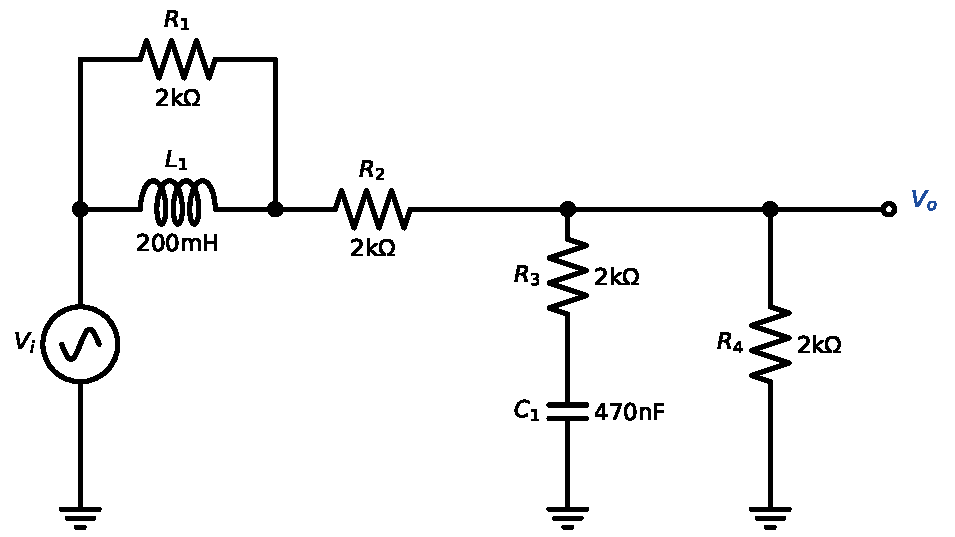
\includegraphics[width=0.8\linewidth,height=4.5cm,keepaspectratio]{p14_circuit}\end{center}
\solstep{1}{Identify the sources}Independent sources: the AC input $V_i(t)$. There is no DC source, so $V_{o,dc}=0$ and $V_o(t)=v_{o,ac}(t)$: Step 2 is skipped.
\solstep{2}{DC circuit}No DC sources: $V_{o,dc}=0$.
\solstep{3}{AC circuit}Replace every capacitor by $\frac{1}{sC}$ and every inductor by $sL$.
AC equivalent circuit (nodes named for the next step):
\begin{center}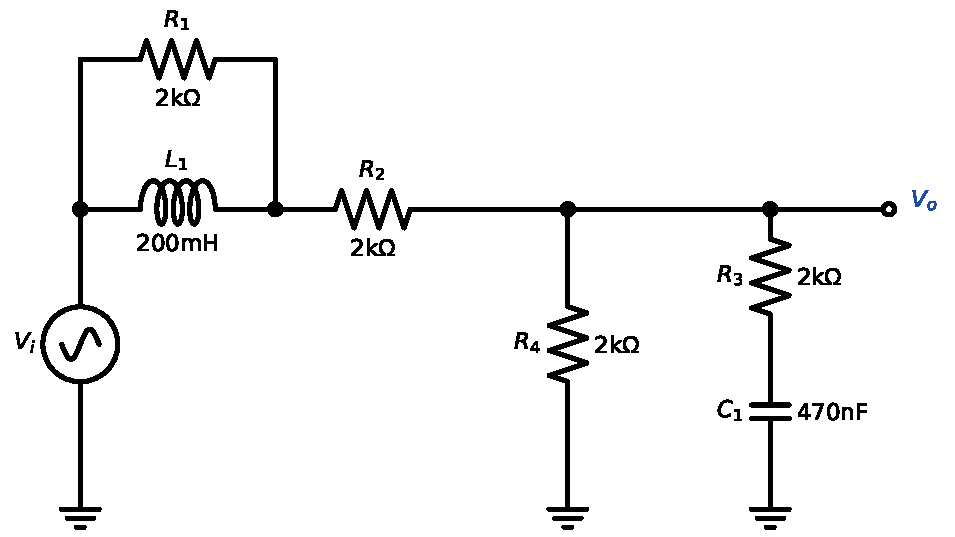
\includegraphics[width=0.95\linewidth,height=5.2cm,keepaspectratio]{p14_ac}\end{center}

\solstep{4}{Transfer function by a chain of dividers}Walk from the input to the output through the named nodes: $V_{i} \to V_{o}$. There is a single link, so $H(s)$ is just one voltage divider (tool T2).
Impedances seen \emph{looking right} from a node (everything from that node to ground, excluding what is on its left). Compute them from the far right toward the input:
\begin{align*}
Z_{o} &= R_{4} \parallel \left(R_{3} + \frac{1}{sC_{1}}\right) = \dfrac{1000\,s + 1.06\times 10^{6}}{s + 532}
\end{align*}

Now each link. {\small (Algebra tip: to simplify a fraction that contains fractions, multiply its top and bottom by every inner denominator; then divide top and bottom by the leading coefficient of the denominator so that it starts with a plain $s^n$.)}
\begin{align*}
\frac{V_{o}}{V_{i}} &= \frac{Z_{o}}{\left(sL_{1} \parallel R_{1}\right) + R_{2} + Z_{o}} = \dfrac{0.2\,s^{2} + 2210\,s + 2.13\times 10^{6}}{s^{2} + 6640\,s + 4.26\times 10^{6}}
\end{align*}

So:\[
H(s) = \dfrac{0.2\,s^{2} + 2210\,s + 2.13\times 10^{6}}{s^{2} + 6640\,s + 4.26\times 10^{6}}
\]

\solstep{5}{Standard (Bode-ready) form}Find the roots. Every root $s=-p$ of the denominator is a \emph{pole}, every root $s=-z$ of the numerator is a \emph{zero}; $|p|$ and $|z|$ are the corner frequencies (rad/s).
\begin{itemize}[leftmargin=*,itemsep=2pt]
\item Numerator: $0.2\,s^{2} + 2210\,s + 2.13\times 10^{6}$; divide by the leading coefficient $0.2$ (this does not move the roots): $s^{2} + 11100\,s + 1.06\times 10^{7}$; quadratic formula:\[
s = \frac{-11100 \pm \sqrt{(11100)^2 - 4(1.06\times 10^{7})}}{2} = \frac{-11100 \pm 8940}{2} \Rightarrow s = -1060,\ -10000
\]

\item Denominator: $s^{2} + 6640\,s + 4.26\times 10^{6}$; quadratic formula:\[
s = \frac{-6640 \pm \sqrt{(6640)^2 - 4(4.26\times 10^{6})}}{2} = \frac{-6640 \pm 5200}{2} \Rightarrow s = -719,\ -5920
\]

\end{itemize}

Factored form (leading coefficient in front):
\[
H(s) = 0.2\,\dfrac{(s+1060)(s+10000)}{(s+719)(s+5920)}
\]

Bode-ready form: rewrite every $(s+p) = p\left(1+\frac{s}{p}\right)$ and $(s+z) = z\left(1+\frac{s}{z}\right)$, and collect all constants into $K$. Then every factor except $K$ is $\approx 1$ inside the pass-band:
\[
H(s) = 0.5\,\dfrac{1}{1+\dfrac{s}{2\pi\cdot 114}}\,\left(1+\dfrac{s}{2\pi\cdot 169}\right)\,\dfrac{1}{1+\dfrac{s}{2\pi\cdot 942}}\,\left(1+\dfrac{s}{2\pi\cdot 1.59\mathrm{k}}\right),\qquad K = 0.5
\]

\begin{center}\renewcommand{\arraystretch}{1.35}
\begin{tabular}{cccc}
\toprule
type & $\omega_c$ (rad/s) & $f_c=\omega_c/2\pi$ & slope change \\
\midrule
pole & $719$ & 114 Hz & $-20$ dB/dec \\
zero & $1060$ & 169 Hz & $+20$ dB/dec \\
pole & $5920$ & 942 Hz & $-20$ dB/dec \\
zero & $10000$ & 1.59 kHz & $+20$ dB/dec \\
\bottomrule
\end{tabular}\end{center}

\solstep{6}{Magnitude Bode plot}Below every corner, all factors are $\approx$ constant: $|H| \approx 0.5$ $= -6.02$\,dB (flat, 0 dB/dec). Then, moving right, each pole bends the line down by 20\,dB/dec and each zero bends it up by 20\,dB/dec (tool T6):
\begin{center}\renewcommand{\arraystretch}{1.35}
\begin{tabular}{lcl}
\toprule
frequency range & slope & asymptote level \\
\midrule
$f<$ 114 Hz & $0$ dB/dec (flat) & -6.02 dB at end \\
114 Hz -- 169 Hz & $-20$ dB/dec & -6.02 dB at start, -9.42 dB at end \\
169 Hz -- 942 Hz & $0$ dB/dec (flat) & -9.42 dB at start, -9.42 dB at end \\
942 Hz -- 1.59 kHz & $-20$ dB/dec & -9.42 dB at start, -14 dB at end \\
$f>$ 1.59 kHz & $0$ dB/dec (flat) & -14 dB at start \\
\bottomrule
\end{tabular}\end{center}

\begin{center}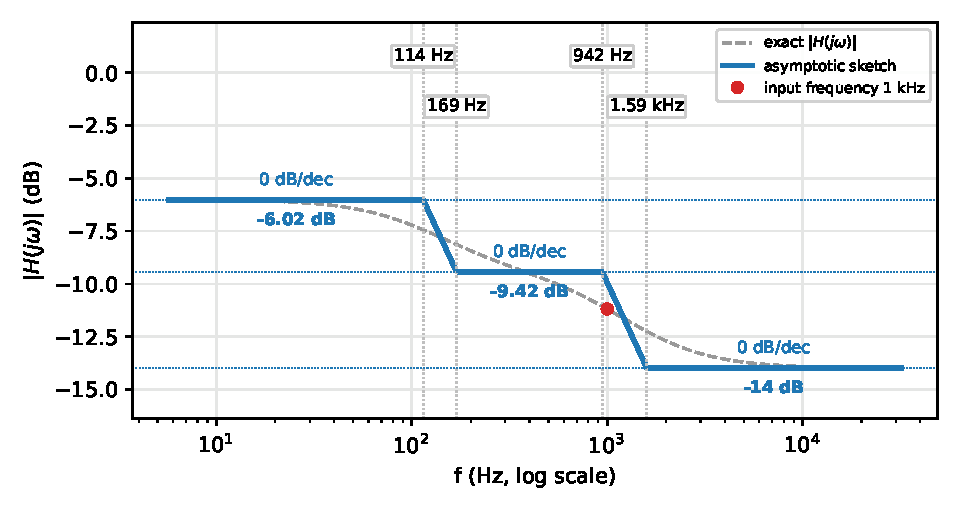
\includegraphics[width=0.78\linewidth,height=6.5cm,keepaspectratio]{p14_bode}\end{center}

{\small Blue: the straight-line sketch you are expected to draw. Dashed grey: the exact curve (about 3\,dB below the corner of an isolated pole). Red dot: the input frequency of Step 7.}
\solstep{7}{Steady-state output}The input is $V_i(t) = 1\sin\left(2\pi\cdot 1000\,t+\frac{\pi}{3}\right)$, so $\omega_{in} = 2\pi\cdot 1000 = 6280$\,rad/s. Put $s=j\omega_{in}$ in each factor (tool T5): magnitudes multiply, angles add.
{\small Rules: $\left|\frac{s}{s+p}\right| = \frac{\omega}{\sqrt{\omega^2+p^2}}$, $\angle = \frac{\pi}{2}-\tan^{-1}\frac{\omega}{p}$;\quad $\left|\frac{1}{1+s/p}\right| = \frac{1}{\sqrt{1+(\omega/p)^2}}$, $\angle = -\tan^{-1}\frac{\omega}{p}$;\quad $\left|1+\frac{s}{z}\right| = \sqrt{1+(\omega/z)^2}$, $\angle = \tan^{-1}\frac{\omega}{z}$;\quad a negative $K$ adds $-\pi$.}
\begin{center}\renewcommand{\arraystretch}{1.35}
\begin{tabular}{ccc}
\toprule
factor & magnitude & angle (rad) \\
\midrule
$0.5$ & $0.5$ & $0$ \\
$\rule[-1.7em]{0pt}{4em}\dfrac{1}{1+\dfrac{s}{2\pi\cdot 114}}$ & $0.1137$ & $-1.46$ \\
$\rule[-1.1em]{0pt}{2.8em}\left(1+\dfrac{s}{2\pi\cdot 169}\right)$ & $5.99$ & $1.4$ \\
$\rule[-1.7em]{0pt}{4em}\dfrac{1}{1+\dfrac{s}{2\pi\cdot 942}}$ & $0.6857$ & $-0.815$ \\
$\rule[-1.1em]{0pt}{2.8em}\left(1+\dfrac{s}{2\pi\cdot 1.59\mathrm{k}}\right)$ & $1.181$ & $0.561$ \\
\textbf{total} & $\mathbf{0.2757}$ (product) & $\mathbf{-0.308}$ (sum) \\
\bottomrule
\end{tabular}\end{center}

\begin{align*}
|H(j\omega_{in})| &= 0.276, \qquad \angle H(j\omega_{in}) = -0.308\ \mathrm{rad} \\
v_{o,ac}(t) &= 0.276\times 1\,\sin\left(2\pi\cdot 1000\,t + 0.739\right) = 0.276\,\sin\left(2\pi\cdot 1000\,t + 0.739\right)
\end{align*}

(phase: $\theta + \angle H = \frac{\pi}{3} + (-0.308) = 0.739$\,rad.)
\[
\boxed{V_o(t) = 0.276\,\sin\left(2\pi\cdot 1000\,t + 0.739\right)\ \mathrm{V}}
\]

\begin{ansbox}
$H(s) = 0.5\,\dfrac{1}{1+\dfrac{s}{2\pi\cdot 114}}\,\left(1+\dfrac{s}{2\pi\cdot 169}\right)\,\dfrac{1}{1+\dfrac{s}{2\pi\cdot 942}}\,\left(1+\dfrac{s}{2\pi\cdot 1.59\mathrm{k}}\right)$\quad (corners: 114 Hz, 169 Hz, 942 Hz, 1.59 kHz)\\[4pt]
$V_o(t) = 0.276\,\sin\left(2\pi\cdot 1000\,t + 0.739\right)\ \mathrm{V}$
\end{ansbox}

\newpage
\subsection*{Solution 1A.15 \hfill Hard}
\begin{center}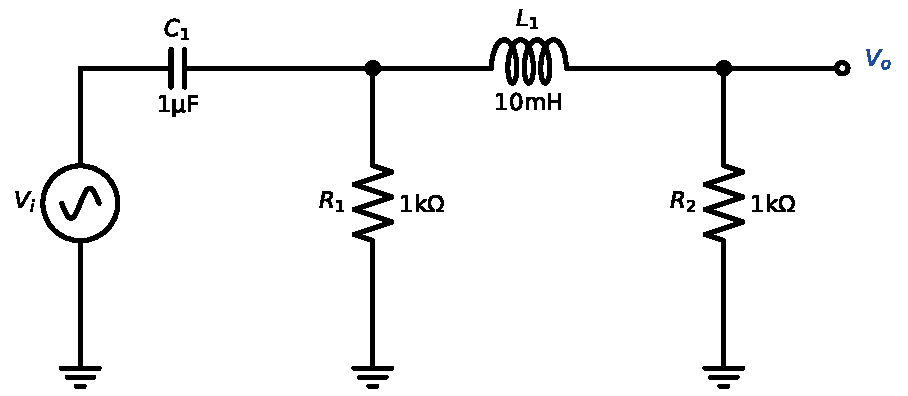
\includegraphics[width=0.8\linewidth,height=4.5cm,keepaspectratio]{p15_circuit}\end{center}
\solstep{1}{Identify the sources}Independent sources: the AC input $V_i(t)$. There is no DC source, so $V_{o,dc}=0$ and $V_o(t)=v_{o,ac}(t)$: Step 2 is skipped.
\solstep{2}{DC circuit}No DC sources: $V_{o,dc}=0$.
\solstep{3}{AC circuit}Replace every capacitor by $\frac{1}{sC}$ and every inductor by $sL$.
AC equivalent circuit (nodes named for the next step):
\begin{center}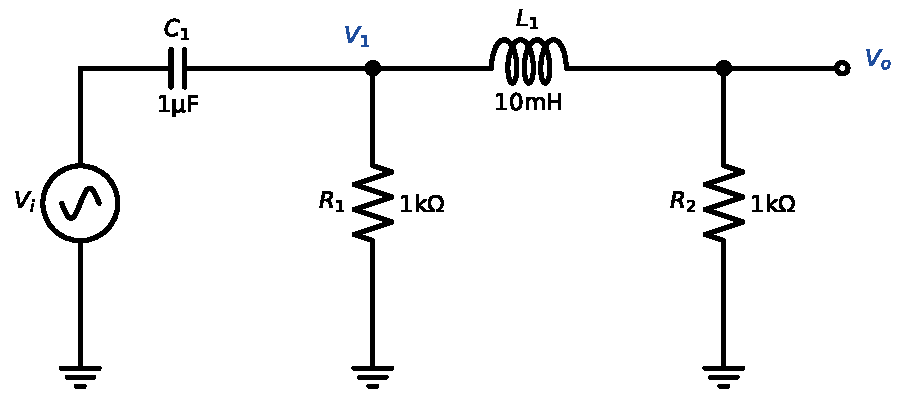
\includegraphics[width=0.95\linewidth,height=5.2cm,keepaspectratio]{p15_ac}\end{center}

\solstep{4}{Transfer function by a chain of dividers}Walk from the input to the output through the named nodes: $V_{i} \to V_{1} \to V_{o}$. The transfer function is the product of the node-to-node ratios (each one is a simple divider, tool T2, or a dependent source, tool T4):
\[
H(s) = \frac{V_o}{V_i} = \frac{V_{1}}{V_{i}}\cdot\frac{V_{o}}{V_{1}}
\]

Impedances seen \emph{looking right} from a node (everything from that node to ground, excluding what is on its left). Compute them from the far right toward the input:
\begin{align*}
Z_{1} &= R_{1} \parallel \left(sL_{1} + R_{2}\right) = \dfrac{1000\,s + 10^{8}}{s + 2\times 10^{5}}
\end{align*}

Now each link. {\small (Algebra tip: to simplify a fraction that contains fractions, multiply its top and bottom by every inner denominator; then divide top and bottom by the leading coefficient of the denominator so that it starts with a plain $s^n$.)}
\begin{align*}
\frac{V_{1}}{V_{i}} &= \frac{Z_{1}}{\frac{1}{sC_{1}} + Z_{1}} = \dfrac{s^{2} + 10^{5}\,s}{s^{2} + 1.01\times 10^{5}\,s + 2\times 10^{8}} \\
\frac{V_{o}}{V_{1}} &= \frac{R_{2}}{sL_{1} + R_{2}} = \dfrac{10^{5}}{s + 10^{5}}
\end{align*}

Multiply the links and simplify (common factors cancel):\[
H(s) = \dfrac{10^{5}\,s}{s^{2} + 1.01\times 10^{5}\,s + 2\times 10^{8}}
\]

\solstep{5}{Standard (Bode-ready) form}Find the roots. Every root $s=-p$ of the denominator is a \emph{pole}, every root $s=-z$ of the numerator is a \emph{zero}; $|p|$ and $|z|$ are the corner frequencies (rad/s).
\begin{itemize}[leftmargin=*,itemsep=2pt]
\item Numerator: it has the factor $s$ $\Rightarrow$ 1 zero at $s=0$.
\item Denominator: $s^{2} + 1.01\times 10^{5}\,s + 2\times 10^{8}$; quadratic formula:\[
s = \frac{-1.01\times 10^{5} \pm \sqrt{(1.01\times 10^{5})^2 - 4(2\times 10^{8})}}{2} = \frac{-1.01\times 10^{5} \pm 97000}{2} \Rightarrow s = -2020,\ -99000
\]

\end{itemize}

Factored form (leading coefficient in front):
\[
H(s) = 10^{5}\,\dfrac{s}{(s+2020)(s+99000)}
\]

Bode-ready form: rewrite every $(s+p) = p\left(1+\frac{s}{p}\right)$ and $(s+z) = z\left(1+\frac{s}{z}\right)$, and collect all constants into $K$. Each $s$ in the numerator is paired with one of the \emph{lowest} poles as $\frac{s}{s+p}$ (that factor is $\approx 1$ above $p$). Then every factor except $K$ is $\approx 1$ inside the pass-band:
\[
H(s) = 1.01\,\dfrac{s}{s+2\pi\cdot 322}\,\dfrac{1}{1+\dfrac{s}{2\pi\cdot 15.8\mathrm{k}}},\qquad K = 1.01
\]

\begin{center}\renewcommand{\arraystretch}{1.35}
\begin{tabular}{cccc}
\toprule
type & $\omega_c$ (rad/s) & $f_c=\omega_c/2\pi$ & slope change \\
\midrule
pole & $2020$ & 322 Hz & $-20$ dB/dec \\
pole & $99000$ & 15.8 kHz & $-20$ dB/dec \\
\bottomrule
\end{tabular}\end{center}

\solstep{6}{Magnitude Bode plot}Below every corner $|H(s)|\approx 5\times 10^{-4}\,s$, so the plot starts with a slope of $+20$\,dB/dec. Then, moving right, each pole bends the line down by 20\,dB/dec and each zero bends it up by 20\,dB/dec (tool T6):
\begin{center}\renewcommand{\arraystretch}{1.35}
\begin{tabular}{lcl}
\toprule
frequency range & slope & asymptote level \\
\midrule
$f<$ 322 Hz & $+20$ dB/dec & 0.0891 dB at end \\
322 Hz -- 15.8 kHz & $0$ dB/dec (flat) & 0.0891 dB at start, 0.0891 dB at end \\
$f>$ 15.8 kHz & $-20$ dB/dec & 0.0891 dB at start \\
\bottomrule
\end{tabular}\end{center}

The flat (pass-band) level is $20\log_{10}|K| = 20\log_{10}1.01 = 0.0891$\,dB.
\begin{center}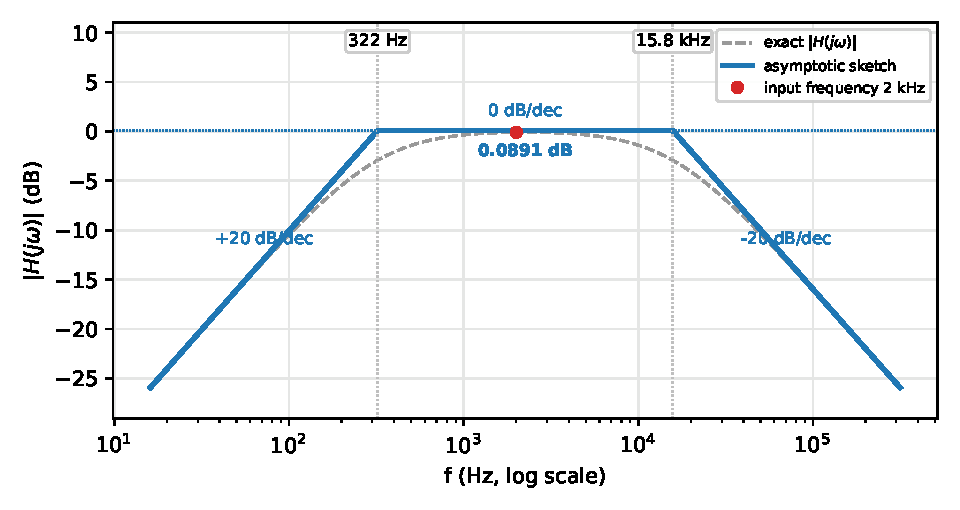
\includegraphics[width=0.78\linewidth,height=6.5cm,keepaspectratio]{p15_bode}\end{center}

{\small Blue: the straight-line sketch you are expected to draw. Dashed grey: the exact curve (about 3\,dB below the corner of an isolated pole). Red dot: the input frequency of Step 7.}
\solstep{7}{Steady-state output}The input is $V_i(t) = 0.5\sin\left(2\pi\cdot 2000\,t\right)$, so $\omega_{in} = 2\pi\cdot 2000 = 12600$\,rad/s. Put $s=j\omega_{in}$ in each factor (tool T5): magnitudes multiply, angles add.
{\small Rules: $\left|\frac{s}{s+p}\right| = \frac{\omega}{\sqrt{\omega^2+p^2}}$, $\angle = \frac{\pi}{2}-\tan^{-1}\frac{\omega}{p}$;\quad $\left|\frac{1}{1+s/p}\right| = \frac{1}{\sqrt{1+(\omega/p)^2}}$, $\angle = -\tan^{-1}\frac{\omega}{p}$;\quad $\left|1+\frac{s}{z}\right| = \sqrt{1+(\omega/z)^2}$, $\angle = \tan^{-1}\frac{\omega}{z}$;\quad a negative $K$ adds $-\pi$.}
\begin{center}\renewcommand{\arraystretch}{1.35}
\begin{tabular}{ccc}
\toprule
factor & magnitude & angle (rad) \\
\midrule
$1.01$ & $1.01$ & $0$ \\
$\rule[-1.1em]{0pt}{2.8em}\dfrac{s}{s+2\pi\cdot 322}$ & $0.9873$ & $0.159$ \\
$\rule[-1.7em]{0pt}{4em}\dfrac{1}{1+\dfrac{s}{2\pi\cdot 15.8\mathrm{k}}}$ & $0.992$ & $-0.126$ \\
\textbf{total} & $\mathbf{0.9896}$ (product) & $\mathbf{0.0331}$ (sum) \\
\bottomrule
\end{tabular}\end{center}

\begin{align*}
|H(j\omega_{in})| &= 0.99, \qquad \angle H(j\omega_{in}) = 0.0331\ \mathrm{rad} \\
v_{o,ac}(t) &= 0.99\times 0.5\,\sin\left(2\pi\cdot 2000\,t + 0.0331\right) = 0.495\,\sin\left(2\pi\cdot 2000\,t + 0.0331\right)
\end{align*}

\[
\boxed{V_o(t) = 0.495\,\sin\left(2\pi\cdot 2000\,t + 0.0331\right)\ \mathrm{V}}
\]

\begin{ansbox}
$H(s) = 1.01\,\dfrac{s}{s+2\pi\cdot 322}\,\dfrac{1}{1+\dfrac{s}{2\pi\cdot 15.8\mathrm{k}}}$\quad (corners: 322 Hz, 15.8 kHz)\\[4pt]
$V_o(t) = 0.495\,\sin\left(2\pi\cdot 2000\,t + 0.0331\right)\ \mathrm{V}$
\end{ansbox}

\newpage
\subsection*{Solution 1A.16 \hfill Hard}
\begin{center}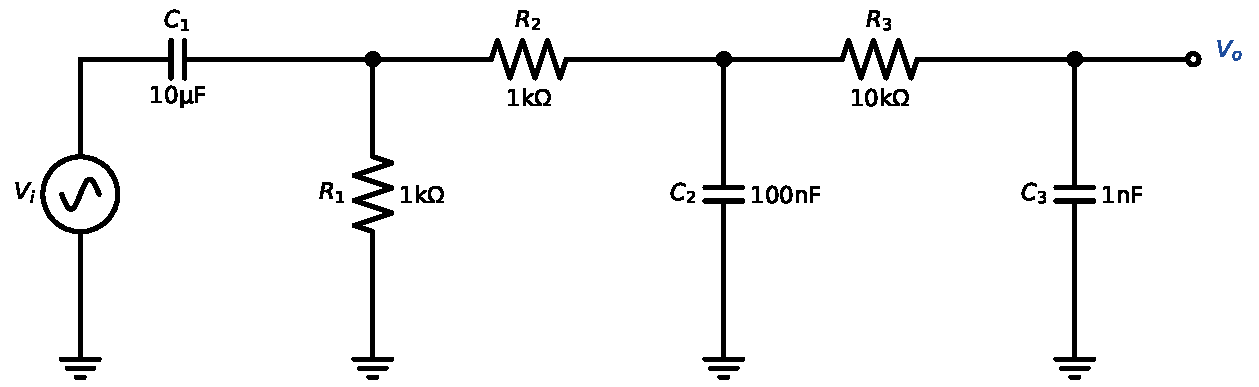
\includegraphics[width=0.8\linewidth,height=4.5cm,keepaspectratio]{p16_circuit}\end{center}
\solstep{1}{Identify the sources}Independent sources: the AC input $V_i(t)$. There is no DC source, so $V_{o,dc}=0$ and $V_o(t)=v_{o,ac}(t)$: Step 2 is skipped.
\solstep{2}{DC circuit}No DC sources: $V_{o,dc}=0$.
\solstep{3}{AC circuit}Replace every capacitor by $\frac{1}{sC}$ and every inductor by $sL$.
AC equivalent circuit (nodes named for the next step):
\begin{center}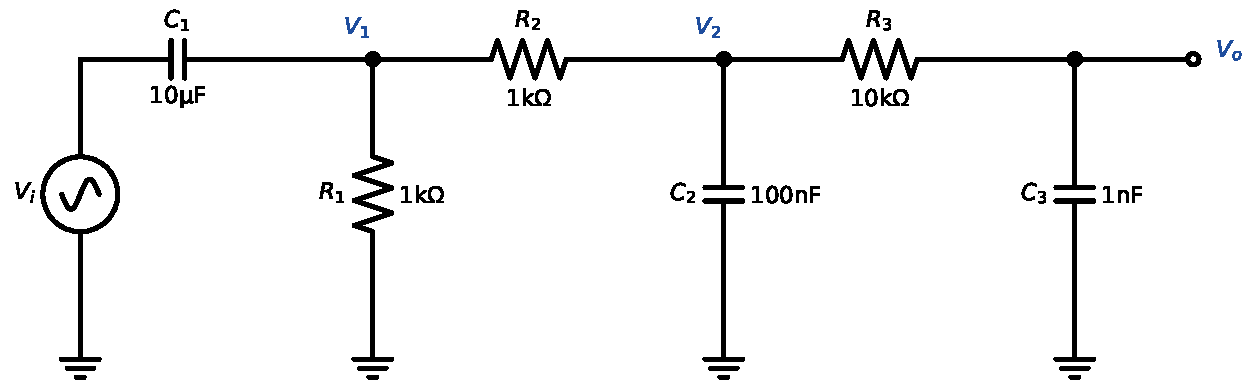
\includegraphics[width=0.95\linewidth,height=5.2cm,keepaspectratio]{p16_ac}\end{center}

\solstep{4}{Transfer function by a chain of dividers}Walk from the input to the output through the named nodes: $V_{i} \to V_{1} \to V_{2} \to V_{o}$. The transfer function is the product of the node-to-node ratios (each one is a simple divider, tool T2, or a dependent source, tool T4):
\[
H(s) = \frac{V_o}{V_i} = \frac{V_{1}}{V_{i}}\cdot\frac{V_{2}}{V_{1}}\cdot\frac{V_{o}}{V_{2}}
\]

Impedances seen \emph{looking right} from a node (everything from that node to ground, excluding what is on its left). Compute them from the far right toward the input:
\begin{align*}
Z_{2} &= \frac{1}{sC_{2}} \parallel \left(R_{3} + \frac{1}{sC_{3}}\right) = \dfrac{10^{7}\,s + 10^{12}}{s^{2} + 1.01\times 10^{5}\,s} \\
Z_{1} &= R_{1} \parallel \left(R_{2} + Z_{2}\right) = \dfrac{500\,s^{2} + 5.55\times 10^{7}\,s + 5\times 10^{11}}{s^{2} + 1.06\times 10^{5}\,s + 5\times 10^{8}}
\end{align*}

Now each link. {\small (Algebra tip: to simplify a fraction that contains fractions, multiply its top and bottom by every inner denominator; then divide top and bottom by the leading coefficient of the denominator so that it starts with a plain $s^n$.)}
\begin{align*}
\frac{V_{1}}{V_{i}} &= \frac{Z_{1}}{\frac{1}{sC_{1}} + Z_{1}} = \dfrac{s^{3} + 1.11\times 10^{5}\,s^{2} + 10^{9}\,s}{s^{3} + 1.11\times 10^{5}\,s^{2} + 1.02\times 10^{9}\,s + 10^{11}} \\
\frac{V_{2}}{V_{1}} &= \frac{Z_{2}}{R_{2} + Z_{2}} = \dfrac{10000\,s + 10^{9}}{s^{2} + 1.11\times 10^{5}\,s + 10^{9}} \\
\frac{V_{o}}{V_{2}} &= \frac{\frac{1}{sC_{3}}}{R_{3} + \frac{1}{sC_{3}}} = \dfrac{10^{5}}{s + 10^{5}}
\end{align*}

Multiply the links and simplify (common factors cancel):\[
H(s) = \dfrac{10^{9}\,s}{s^{3} + 1.11\times 10^{5}\,s^{2} + 1.02\times 10^{9}\,s + 10^{11}}
\]

\solstep{5}{Standard (Bode-ready) form}Find the roots. Every root $s=-p$ of the denominator is a \emph{pole}, every root $s=-z$ of the numerator is a \emph{zero}; $|p|$ and $|z|$ are the corner frequencies (rad/s).
\begin{itemize}[leftmargin=*,itemsep=2pt]
\item Numerator: it has the factor $s$ $\Rightarrow$ 1 zero at $s=0$.
\item Denominator: $s^{3} + 1.11\times 10^{5}\,s^{2} + 1.02\times 10^{9}\,s + 10^{11}$; this is degree 3: use a calculator's polynomial solver (or \texttt{numpy.roots}) $\Rightarrow s = -99,\ -9990,\ -1.01\times 10^{5}$.
\end{itemize}

Factored form (leading coefficient in front):
\[
H(s) = 10^{9}\,\dfrac{s}{(s+99)(s+9990)(s+1.01\times 10^{5})}
\]

Bode-ready form: rewrite every $(s+p) = p\left(1+\frac{s}{p}\right)$ and $(s+z) = z\left(1+\frac{s}{z}\right)$, and collect all constants into $K$. Each $s$ in the numerator is paired with one of the \emph{lowest} poles as $\frac{s}{s+p}$ (that factor is $\approx 1$ above $p$). Then every factor except $K$ is $\approx 1$ inside the pass-band:
\[
H(s) = 0.99\,\dfrac{s}{s+2\pi\cdot 15.8}\,\dfrac{1}{1+\dfrac{s}{2\pi\cdot 1.59\mathrm{k}}}\,\dfrac{1}{1+\dfrac{s}{2\pi\cdot 16.1\mathrm{k}}},\qquad K = 0.99
\]

\begin{center}\renewcommand{\arraystretch}{1.35}
\begin{tabular}{cccc}
\toprule
type & $\omega_c$ (rad/s) & $f_c=\omega_c/2\pi$ & slope change \\
\midrule
pole & $99$ & 15.8 Hz & $-20$ dB/dec \\
pole & $9990$ & 1.59 kHz & $-20$ dB/dec \\
pole & $1.01\times 10^{5}$ & 16.1 kHz & $-20$ dB/dec \\
\bottomrule
\end{tabular}\end{center}

\solstep{6}{Magnitude Bode plot}Below every corner $|H(s)|\approx 0.01\,s$, so the plot starts with a slope of $+20$\,dB/dec. Then, moving right, each pole bends the line down by 20\,dB/dec and each zero bends it up by 20\,dB/dec (tool T6):
\begin{center}\renewcommand{\arraystretch}{1.35}
\begin{tabular}{lcl}
\toprule
frequency range & slope & asymptote level \\
\midrule
$f<$ 15.8 Hz & $+20$ dB/dec & -0.0882 dB at end \\
15.8 Hz -- 1.59 kHz & $0$ dB/dec (flat) & -0.0882 dB at start, -0.0882 dB at end \\
1.59 kHz -- 16.1 kHz & $-20$ dB/dec & -0.0882 dB at start, -20.2 dB at end \\
$f>$ 16.1 kHz & $-40$ dB/dec & -20.2 dB at start \\
\bottomrule
\end{tabular}\end{center}

The flat (pass-band) level is $20\log_{10}|K| = 20\log_{10}0.99 = -0.0882$\,dB.
\begin{center}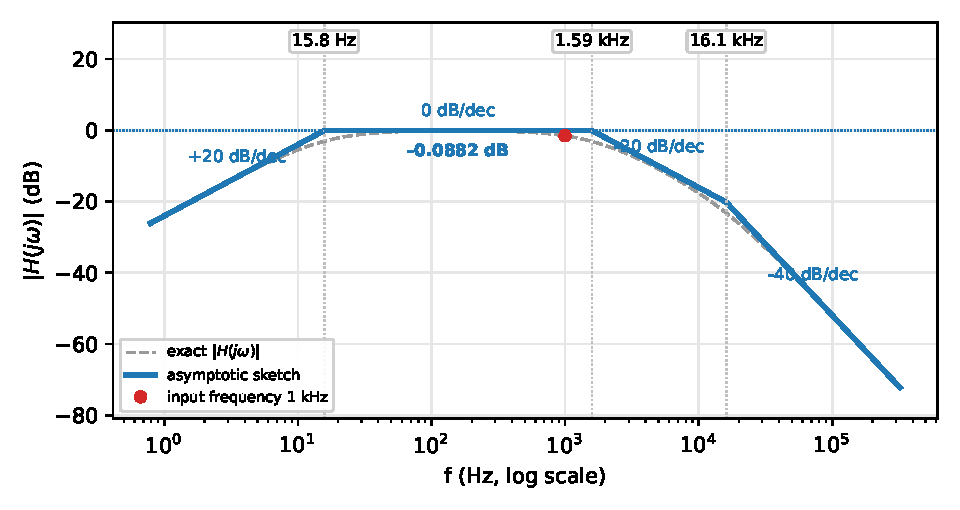
\includegraphics[width=0.78\linewidth,height=6.5cm,keepaspectratio]{p16_bode}\end{center}

{\small Blue: the straight-line sketch you are expected to draw. Dashed grey: the exact curve (about 3\,dB below the corner of an isolated pole). Red dot: the input frequency of Step 7.}
\solstep{7}{Steady-state output}The input is $V_i(t) = 1\sin\left(2\pi\cdot 1000\,t\right)$, so $\omega_{in} = 2\pi\cdot 1000 = 6280$\,rad/s. Put $s=j\omega_{in}$ in each factor (tool T5): magnitudes multiply, angles add.
{\small Rules: $\left|\frac{s}{s+p}\right| = \frac{\omega}{\sqrt{\omega^2+p^2}}$, $\angle = \frac{\pi}{2}-\tan^{-1}\frac{\omega}{p}$;\quad $\left|\frac{1}{1+s/p}\right| = \frac{1}{\sqrt{1+(\omega/p)^2}}$, $\angle = -\tan^{-1}\frac{\omega}{p}$;\quad $\left|1+\frac{s}{z}\right| = \sqrt{1+(\omega/z)^2}$, $\angle = \tan^{-1}\frac{\omega}{z}$;\quad a negative $K$ adds $-\pi$.}
\begin{center}\renewcommand{\arraystretch}{1.35}
\begin{tabular}{ccc}
\toprule
factor & magnitude & angle (rad) \\
\midrule
$0.99$ & $0.9899$ & $0$ \\
$\rule[-1.1em]{0pt}{2.8em}\dfrac{s}{s+2\pi\cdot 15.8}$ & $0.9999$ & $0.0158$ \\
$\rule[-1.7em]{0pt}{4em}\dfrac{1}{1+\dfrac{s}{2\pi\cdot 1.59\mathrm{k}}}$ & $0.8465$ & $-0.561$ \\
$\rule[-1.7em]{0pt}{4em}\dfrac{1}{1+\dfrac{s}{2\pi\cdot 16.1\mathrm{k}}}$ & $0.9981$ & $-0.0621$ \\
\textbf{total} & $\mathbf{0.8363}$ (product) & $\mathbf{-0.608}$ (sum) \\
\bottomrule
\end{tabular}\end{center}

\begin{align*}
|H(j\omega_{in})| &= 0.836, \qquad \angle H(j\omega_{in}) = -0.608\ \mathrm{rad} \\
v_{o,ac}(t) &= 0.836\times 1\,\sin\left(2\pi\cdot 1000\,t - 0.608\right) = 0.836\,\sin\left(2\pi\cdot 1000\,t - 0.608\right)
\end{align*}

\[
\boxed{V_o(t) = 0.836\,\sin\left(2\pi\cdot 1000\,t - 0.608\right)\ \mathrm{V}}
\]

\begin{ansbox}
$H(s) = 0.99\,\dfrac{s}{s+2\pi\cdot 15.8}\,\dfrac{1}{1+\dfrac{s}{2\pi\cdot 1.59\mathrm{k}}}\,\dfrac{1}{1+\dfrac{s}{2\pi\cdot 16.1\mathrm{k}}}$\quad (corners: 15.8 Hz, 1.59 kHz, 16.1 kHz)\\[4pt]
$V_o(t) = 0.836\,\sin\left(2\pi\cdot 1000\,t - 0.608\right)\ \mathrm{V}$
\end{ansbox}

\newpage
\subsection*{Solution 1A.17 \hfill Hard}
\begin{center}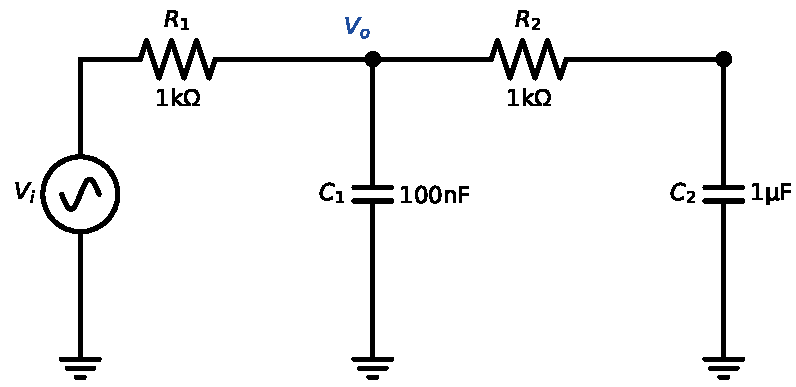
\includegraphics[width=0.8\linewidth,height=4.5cm,keepaspectratio]{p17_circuit}\end{center}
\solstep{1}{Identify the sources}Independent sources: the AC input $V_i(t)$. There is no DC source, so $V_{o,dc}=0$ and $V_o(t)=v_{o,ac}(t)$: Step 2 is skipped.
\solstep{2}{DC circuit}No DC sources: $V_{o,dc}=0$.
\solstep{3}{AC circuit}Replace every capacitor by $\frac{1}{sC}$ and every inductor by $sL$.
AC equivalent circuit (nodes named for the next step):
\begin{center}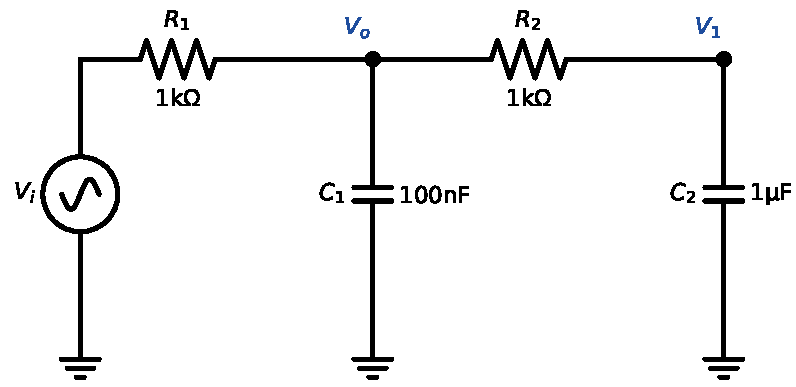
\includegraphics[width=0.95\linewidth,height=5.2cm,keepaspectratio]{p17_ac}\end{center}

\solstep{4}{Transfer function by a chain of dividers}Walk from the input to the output through the named nodes: $V_{i} \to V_{o}$. There is a single link, so $H(s)$ is just one voltage divider (tool T2).
Impedances seen \emph{looking right} from a node (everything from that node to ground, excluding what is on its left). Compute them from the far right toward the input:
\begin{align*}
Z_{o} &= \frac{1}{sC_{1}} \parallel \left(R_{2} + \frac{1}{sC_{2}}\right) = \dfrac{10^{7}\,s + 10^{10}}{s^{2} + 11000\,s}
\end{align*}

Now each link. {\small (Algebra tip: to simplify a fraction that contains fractions, multiply its top and bottom by every inner denominator; then divide top and bottom by the leading coefficient of the denominator so that it starts with a plain $s^n$.)}
\begin{align*}
\frac{V_{o}}{V_{i}} &= \frac{Z_{o}}{R_{1} + Z_{o}} = \dfrac{10000\,s + 10^{7}}{s^{2} + 21000\,s + 10^{7}}
\end{align*}

So:\[
H(s) = \dfrac{10000\,s + 10^{7}}{s^{2} + 21000\,s + 10^{7}}
\]

\solstep{5}{Standard (Bode-ready) form}Find the roots. Every root $s=-p$ of the denominator is a \emph{pole}, every root $s=-z$ of the numerator is a \emph{zero}; $|p|$ and $|z|$ are the corner frequencies (rad/s).
\begin{itemize}[leftmargin=*,itemsep=2pt]
\item Numerator: $10000\,s + 10^{7}$; divide by the leading coefficient $10000$ (this does not move the roots): $s + 1000$; $s + 1000 = 0 \Rightarrow s = -1000$.
\item Denominator: $s^{2} + 21000\,s + 10^{7}$; quadratic formula:\[
s = \frac{-21000 \pm \sqrt{(21000)^2 - 4(10^{7})}}{2} = \frac{-21000 \pm 20000}{2} \Rightarrow s = -488,\ -20500
\]

\end{itemize}

Factored form (leading coefficient in front):
\[
H(s) = 10000\,\dfrac{(s+1000)}{(s+488)(s+20500)}
\]

Bode-ready form: rewrite every $(s+p) = p\left(1+\frac{s}{p}\right)$ and $(s+z) = z\left(1+\frac{s}{z}\right)$, and collect all constants into $K$. Then every factor except $K$ is $\approx 1$ inside the pass-band:
\[
H(s) = 1\,\dfrac{1}{1+\dfrac{s}{2\pi\cdot 77.6}}\,\left(1+\dfrac{s}{2\pi\cdot 159}\right)\,\dfrac{1}{1+\dfrac{s}{2\pi\cdot 3.26\mathrm{k}}},\qquad K = 1
\]

\begin{center}\renewcommand{\arraystretch}{1.35}
\begin{tabular}{cccc}
\toprule
type & $\omega_c$ (rad/s) & $f_c=\omega_c/2\pi$ & slope change \\
\midrule
pole & $488$ & 77.6 Hz & $-20$ dB/dec \\
zero & $1000$ & 159 Hz & $+20$ dB/dec \\
pole & $20500$ & 3.26 kHz & $-20$ dB/dec \\
\bottomrule
\end{tabular}\end{center}

\solstep{6}{Magnitude Bode plot}Below every corner, all factors are $\approx$ constant: $|H| \approx 1$ $= -0.00000000000000193$\,dB (flat, 0 dB/dec). Then, moving right, each pole bends the line down by 20\,dB/dec and each zero bends it up by 20\,dB/dec (tool T6):
\begin{center}\renewcommand{\arraystretch}{1.35}
\begin{tabular}{lcl}
\toprule
frequency range & slope & asymptote level \\
\midrule
$f<$ 77.6 Hz & $0$ dB/dec (flat) & 0 dB at end \\
77.6 Hz -- 159 Hz & $-20$ dB/dec & 0 dB at start, -6.24 dB at end \\
159 Hz -- 3.26 kHz & $0$ dB/dec (flat) & -6.24 dB at start, -6.24 dB at end \\
$f>$ 3.26 kHz & $-20$ dB/dec & -6.24 dB at start \\
\bottomrule
\end{tabular}\end{center}

\begin{center}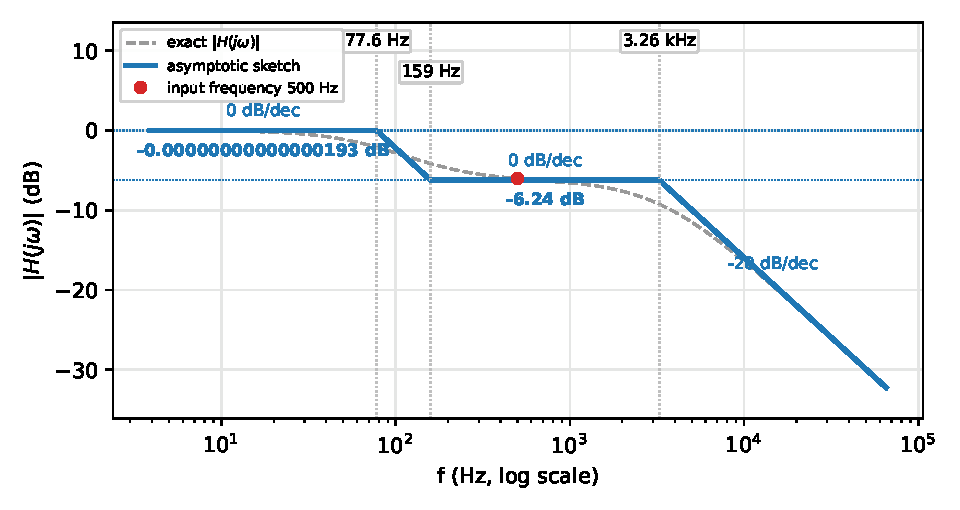
\includegraphics[width=0.78\linewidth,height=6.5cm,keepaspectratio]{p17_bode}\end{center}

{\small Blue: the straight-line sketch you are expected to draw. Dashed grey: the exact curve (about 3\,dB below the corner of an isolated pole). Red dot: the input frequency of Step 7.}
\solstep{7}{Steady-state output}The input is $V_i(t) = 1\sin\left(2\pi\cdot 500\,t\right)$, so $\omega_{in} = 2\pi\cdot 500 = 3140$\,rad/s. Put $s=j\omega_{in}$ in each factor (tool T5): magnitudes multiply, angles add.
{\small Rules: $\left|\frac{s}{s+p}\right| = \frac{\omega}{\sqrt{\omega^2+p^2}}$, $\angle = \frac{\pi}{2}-\tan^{-1}\frac{\omega}{p}$;\quad $\left|\frac{1}{1+s/p}\right| = \frac{1}{\sqrt{1+(\omega/p)^2}}$, $\angle = -\tan^{-1}\frac{\omega}{p}$;\quad $\left|1+\frac{s}{z}\right| = \sqrt{1+(\omega/z)^2}$, $\angle = \tan^{-1}\frac{\omega}{z}$;\quad a negative $K$ adds $-\pi$.}
\begin{center}\renewcommand{\arraystretch}{1.35}
\begin{tabular}{ccc}
\toprule
factor & magnitude & angle (rad) \\
\midrule
$1$ & $1$ & $0$ \\
$\rule[-1.7em]{0pt}{4em}\dfrac{1}{1+\dfrac{s}{2\pi\cdot 77.6}}$ & $0.1533$ & $-1.42$ \\
$\rule[-1.1em]{0pt}{2.8em}\left(1+\dfrac{s}{2\pi\cdot 159}\right)$ & $3.297$ & $1.26$ \\
$\rule[-1.7em]{0pt}{4em}\dfrac{1}{1+\dfrac{s}{2\pi\cdot 3.26\mathrm{k}}}$ & $0.9885$ & $-0.152$ \\
\textbf{total} & $\mathbf{0.4997}$ (product) & $\mathbf{-0.306}$ (sum) \\
\bottomrule
\end{tabular}\end{center}

\begin{align*}
|H(j\omega_{in})| &= 0.5, \qquad \angle H(j\omega_{in}) = -0.306\ \mathrm{rad} \\
v_{o,ac}(t) &= 0.5\times 1\,\sin\left(2\pi\cdot 500\,t - 0.306\right) = 0.5\,\sin\left(2\pi\cdot 500\,t - 0.306\right)
\end{align*}

\[
\boxed{V_o(t) = 0.5\,\sin\left(2\pi\cdot 500\,t - 0.306\right)\ \mathrm{V}}
\]

\begin{ansbox}
$H(s) = 1\,\dfrac{1}{1+\dfrac{s}{2\pi\cdot 77.6}}\,\left(1+\dfrac{s}{2\pi\cdot 159}\right)\,\dfrac{1}{1+\dfrac{s}{2\pi\cdot 3.26\mathrm{k}}}$\quad (corners: 77.6 Hz, 159 Hz, 3.26 kHz)\\[4pt]
$V_o(t) = 0.5\,\sin\left(2\pi\cdot 500\,t - 0.306\right)\ \mathrm{V}$
\end{ansbox}

\newpage
\subsection*{Solution 1A.18 \hfill Hard}
\begin{center}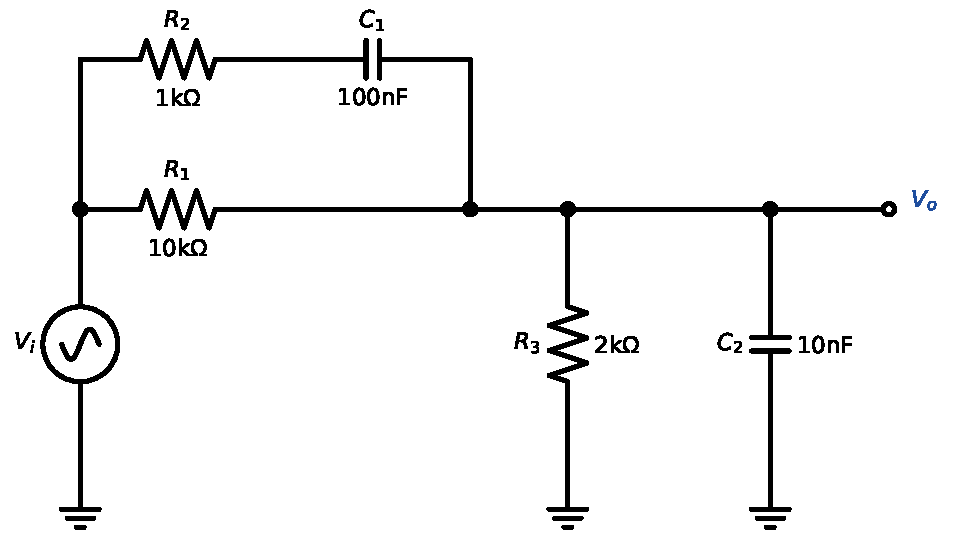
\includegraphics[width=0.8\linewidth,height=4.5cm,keepaspectratio]{p18_circuit}\end{center}
\solstep{1}{Identify the sources}Independent sources: the AC input $V_i(t)$. There is no DC source, so $V_{o,dc}=0$ and $V_o(t)=v_{o,ac}(t)$: Step 2 is skipped.
\solstep{2}{DC circuit}No DC sources: $V_{o,dc}=0$.
\solstep{3}{AC circuit}Replace every capacitor by $\frac{1}{sC}$ and every inductor by $sL$.
AC equivalent circuit (nodes named for the next step):
\begin{center}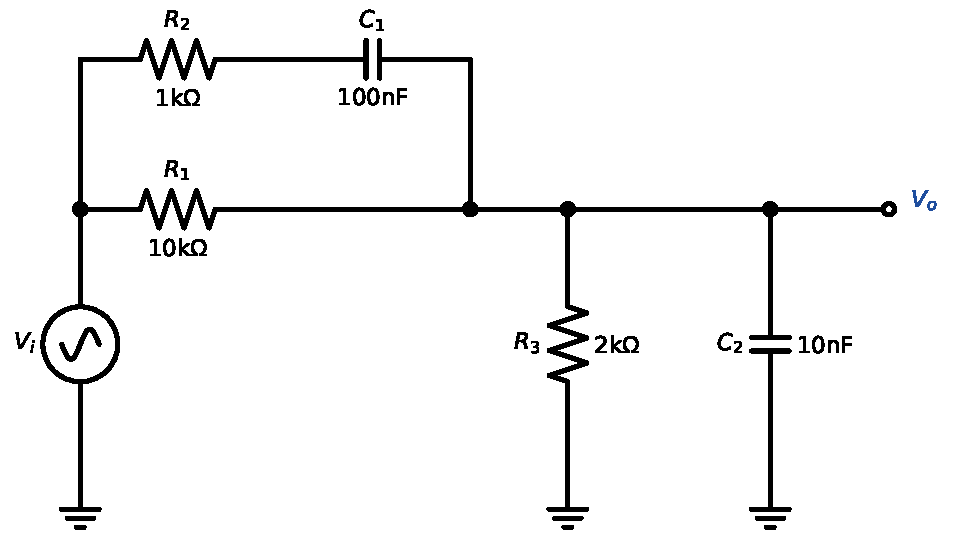
\includegraphics[width=0.95\linewidth,height=5.2cm,keepaspectratio]{p18_ac}\end{center}

\solstep{4}{Transfer function by a chain of dividers}Walk from the input to the output through the named nodes: $V_{i} \to V_{o}$. There is a single link, so $H(s)$ is just one voltage divider (tool T2).
Impedances seen \emph{looking right} from a node (everything from that node to ground, excluding what is on its left). Compute them from the far right toward the input:
\begin{align*}
Z_{o} &= R_{3} \parallel \frac{1}{sC_{2}} = \dfrac{10^{8}}{s + 50000}
\end{align*}

Now each link. {\small (Algebra tip: to simplify a fraction that contains fractions, multiply its top and bottom by every inner denominator; then divide top and bottom by the leading coefficient of the denominator so that it starts with a plain $s^n$.)}
\begin{align*}
\frac{V_{o}}{V_{i}} &= \frac{Z_{o}}{R_{1} \parallel \left(R_{2} + \frac{1}{sC_{1}}\right) + Z_{o}} = \dfrac{1.1\times 10^{5}\,s + 10^{8}}{s^{2} + 1.7\times 10^{5}\,s + 6\times 10^{8}}
\end{align*}

So:\[
H(s) = \dfrac{1.1\times 10^{5}\,s + 10^{8}}{s^{2} + 1.7\times 10^{5}\,s + 6\times 10^{8}}
\]

\solstep{5}{Standard (Bode-ready) form}Find the roots. Every root $s=-p$ of the denominator is a \emph{pole}, every root $s=-z$ of the numerator is a \emph{zero}; $|p|$ and $|z|$ are the corner frequencies (rad/s).
\begin{itemize}[leftmargin=*,itemsep=2pt]
\item Numerator: $1.1\times 10^{5}\,s + 10^{8}$; divide by the leading coefficient $1.1\times 10^{5}$ (this does not move the roots): $s + 909$; $s + 909 = 0 \Rightarrow s = -909$.
\item Denominator: $s^{2} + 1.7\times 10^{5}\,s + 6\times 10^{8}$; quadratic formula:\[
s = \frac{-1.7\times 10^{5} \pm \sqrt{(1.7\times 10^{5})^2 - 4(6\times 10^{8})}}{2} = \frac{-1.7\times 10^{5} \pm 1.63\times 10^{5}}{2} \Rightarrow s = -3610,\ -1.66\times 10^{5}
\]

\end{itemize}

Factored form (leading coefficient in front):
\[
H(s) = 1.1\times 10^{5}\,\dfrac{(s+909)}{(s+3610)(s+1.66\times 10^{5})}
\]

Bode-ready form: rewrite every $(s+p) = p\left(1+\frac{s}{p}\right)$ and $(s+z) = z\left(1+\frac{s}{z}\right)$, and collect all constants into $K$. Then every factor except $K$ is $\approx 1$ inside the pass-band:
\[
H(s) = 0.167\,\left(1+\dfrac{s}{2\pi\cdot 145}\right)\,\dfrac{1}{1+\dfrac{s}{2\pi\cdot 574}}\,\dfrac{1}{1+\dfrac{s}{2\pi\cdot 26.5\mathrm{k}}},\qquad K = 0.167
\]

\begin{center}\renewcommand{\arraystretch}{1.35}
\begin{tabular}{cccc}
\toprule
type & $\omega_c$ (rad/s) & $f_c=\omega_c/2\pi$ & slope change \\
\midrule
zero & $909$ & 145 Hz & $+20$ dB/dec \\
pole & $3610$ & 574 Hz & $-20$ dB/dec \\
pole & $1.66\times 10^{5}$ & 26.5 kHz & $-20$ dB/dec \\
\bottomrule
\end{tabular}\end{center}

\solstep{6}{Magnitude Bode plot}Below every corner, all factors are $\approx$ constant: $|H| \approx 0.167$ $= -15.6$\,dB (flat, 0 dB/dec). Then, moving right, each pole bends the line down by 20\,dB/dec and each zero bends it up by 20\,dB/dec (tool T6):
\begin{center}\renewcommand{\arraystretch}{1.35}
\begin{tabular}{lcl}
\toprule
frequency range & slope & asymptote level \\
\midrule
$f<$ 145 Hz & $0$ dB/dec (flat) & -15.6 dB at end \\
145 Hz -- 574 Hz & $+20$ dB/dec & -15.6 dB at start, -3.59 dB at end \\
574 Hz -- 26.5 kHz & $0$ dB/dec (flat) & -3.59 dB at start, -3.59 dB at end \\
$f>$ 26.5 kHz & $-20$ dB/dec & -3.59 dB at start \\
\bottomrule
\end{tabular}\end{center}

\begin{center}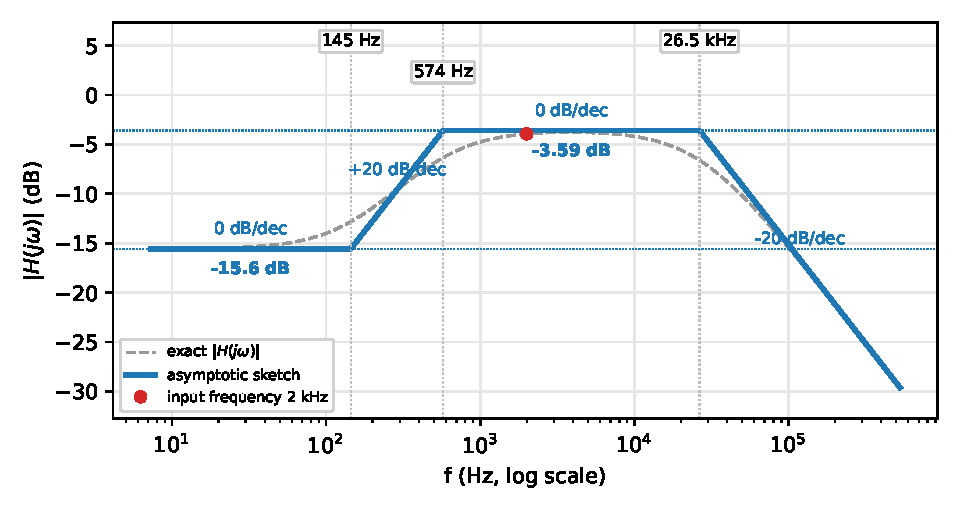
\includegraphics[width=0.78\linewidth,height=6.5cm,keepaspectratio]{p18_bode}\end{center}

{\small Blue: the straight-line sketch you are expected to draw. Dashed grey: the exact curve (about 3\,dB below the corner of an isolated pole). Red dot: the input frequency of Step 7.}
\solstep{7}{Steady-state output}The input is $V_i(t) = 1\sin\left(2\pi\cdot 2000\,t-\frac{\pi}{6}\right)$, so $\omega_{in} = 2\pi\cdot 2000 = 12600$\,rad/s. Put $s=j\omega_{in}$ in each factor (tool T5): magnitudes multiply, angles add.
{\small Rules: $\left|\frac{s}{s+p}\right| = \frac{\omega}{\sqrt{\omega^2+p^2}}$, $\angle = \frac{\pi}{2}-\tan^{-1}\frac{\omega}{p}$;\quad $\left|\frac{1}{1+s/p}\right| = \frac{1}{\sqrt{1+(\omega/p)^2}}$, $\angle = -\tan^{-1}\frac{\omega}{p}$;\quad $\left|1+\frac{s}{z}\right| = \sqrt{1+(\omega/z)^2}$, $\angle = \tan^{-1}\frac{\omega}{z}$;\quad a negative $K$ adds $-\pi$.}
\begin{center}\renewcommand{\arraystretch}{1.35}
\begin{tabular}{ccc}
\toprule
factor & magnitude & angle (rad) \\
\midrule
$0.167$ & $0.1667$ & $0$ \\
$\rule[-1.1em]{0pt}{2.8em}\left(1+\dfrac{s}{2\pi\cdot 145}\right)$ & $13.86$ & $1.5$ \\
$\rule[-1.7em]{0pt}{4em}\dfrac{1}{1+\dfrac{s}{2\pi\cdot 574}}$ & $0.2758$ & $-1.29$ \\
$\rule[-1.7em]{0pt}{4em}\dfrac{1}{1+\dfrac{s}{2\pi\cdot 26.5\mathrm{k}}}$ & $0.9972$ & $-0.0754$ \\
\textbf{total} & $\mathbf{0.6353}$ (product) & $\mathbf{0.132}$ (sum) \\
\bottomrule
\end{tabular}\end{center}

\begin{align*}
|H(j\omega_{in})| &= 0.635, \qquad \angle H(j\omega_{in}) = 0.132\ \mathrm{rad} \\
v_{o,ac}(t) &= 0.635\times 1\,\sin\left(2\pi\cdot 2000\,t - 0.392\right) = 0.635\,\sin\left(2\pi\cdot 2000\,t - 0.392\right)
\end{align*}

(phase: $\theta + \angle H = -\frac{\pi}{6} + (0.132) = -0.392$\,rad.)
\[
\boxed{V_o(t) = 0.635\,\sin\left(2\pi\cdot 2000\,t - 0.392\right)\ \mathrm{V}}
\]

\begin{ansbox}
$H(s) = 0.167\,\left(1+\dfrac{s}{2\pi\cdot 145}\right)\,\dfrac{1}{1+\dfrac{s}{2\pi\cdot 574}}\,\dfrac{1}{1+\dfrac{s}{2\pi\cdot 26.5\mathrm{k}}}$\quad (corners: 145 Hz, 574 Hz, 26.5 kHz)\\[4pt]
$V_o(t) = 0.635\,\sin\left(2\pi\cdot 2000\,t - 0.392\right)\ \mathrm{V}$
\end{ansbox}

\end{document}
